\documentclass[12pt,oneside]{uhthesis}
\usepackage{subfigure}
\usepackage[ruled,lined,linesnumbered,titlenumbered,algochapter,spanish,onelanguage]{algorithm2e}
\usepackage{amsmath}
\usepackage{amssymb}
\usepackage{amsbsy}
\usepackage{caption,booktabs}
\captionsetup{ justification = centering }
%\usepackage{mathpazo}
\usepackage{float}
\setlength{\marginparwidth}{2cm}
\usepackage{todonotes}
\usepackage{listings}
\usepackage{xcolor}
\usepackage{multicol}
\usepackage{graphicx}
\floatstyle{plaintop}
\restylefloat{table}
\addbibresource{Bibliography.bib}
% \setlength{\parskip}{\baselineskip}%
\renewcommand{\tablename}{Tabla}
\renewcommand{\listalgorithmcfname}{Índice de Algoritmos}
%\dontprintsemicolon
\SetAlgoNoEnd

\definecolor{codegreen}{rgb}{0,0.6,0}
\definecolor{codegray}{rgb}{0.5,0.5,0.5}
\definecolor{codepurple}{rgb}{0.58,0,0.82}
\definecolor{backcolour}{rgb}{0.95,0.95,0.92}

\lstdefinestyle{mystyle}{
    backgroundcolor=\color{backcolour},   
    commentstyle=\color{codegreen},
    keywordstyle=\color{purple},
    numberstyle=\tiny\color{codegray},
    stringstyle=\color{codepurple},
    basicstyle=\ttfamily\footnotesize,
    breakatwhitespace=false,         
    breaklines=true,                 
    captionpos=b,                    
    keepspaces=true,                 
    numbers=left,                    
    numbersep=5pt,                  
    showspaces=false,                
    showstringspaces=false,
    showtabs=false,                  
    tabsize=6
}

\lstset{style=mystyle}

\title{Generación automática de procesos de integración de datos. Inferencia de Joins}
\author{\\\vspace{0.25cm}Jes\'us Santos Capote}
\advisor{\\\vspace{0.25cm}Lic. Víctor Manuel Cardentey Fundora\\\vspace{0.2cm}Dra. C. Lucina García Hernández}
\degree{Licenciado en Ciencia de la Computación}
\faculty{Facultad de Matemática y Computación}
\date{Enero del 2024\\\vspace{0.25cm}\href{https://github.com/username/repo}{https://github.com/JesusSantosCapote/autoETL.git}}
\logo{Graphics/uhlogo}
\makenomenclature

\renewcommand{\vec}[1]{\boldsymbol{#1}}
\newcommand{\diff}[1]{\ensuremath{\mathrm{d}#1}}
\newcommand{\me}[1]{\mathrm{e}^{#1}}
\newcommand{\pf}{\mathfrak{p}}
\newcommand{\qf}{\mathfrak{q}}
%\newcommand{\kf}{\mathfrak{k}}
\newcommand{\kt}{\mathtt{k}}
\newcommand{\mf}{\mathfrak{m}}
\newcommand{\hf}{\mathfrak{h}}
\newcommand{\fac}{\mathrm{fac}}
\newcommand{\maxx}[1]{\max\left\{ #1 \right\} }
\newcommand{\minn}[1]{\min\left\{ #1 \right\} }
\newcommand{\lldpcf}{1.25}
\newcommand{\nnorm}[1]{\left\lvert #1 \right\rvert }
\renewcommand{\lstlistingname}{Ejemplo de código}
\renewcommand{\lstlistlistingname}{Ejemplos de código}

\begin{document}

\frontmatter
\maketitle

\begin{dedication}
    Dedicatoria
\end{dedication}
\begin{acknowledgements}
A mis padres, por estar siempre presentes brindando su amor y apoyo, por ser luz 
en momentos de dudas, por ser su prioridad bajo cualquier circunstancia. Al resto de mi 
familia por su cariño y preocupaci\'on por mi bienestar. 

A mi hermana Massiel, por su cariño incondicional, por estar siempre presente, 
por ser mi ejemplo a seguir como cient\'ifico de la computaci\'on y como persona. 

A mis compañeros de carrera, Kenny Villalobos, Ernesto Alfonso, Abraham Gonzalez, Jorge A. Soler, Diamis Alfonso 
y Sheyla Leyva por todas las alegr\'ias y momentos difíciles compartidos; por su amistad incondicional y por 
impulsarme a ser un mejor profesional.

A mis amigos por soportar todos los "hoy no puedo ir", por su cariño y atenciones, por ser refugio del 
estrés durante toda esta etapa.

A los buenos profesores que me he encontrado en estos cuatro años y que contribuyeron al profesional que soy hoy. 
A MATCOM por ser una segunda casa.
\end{acknowledgements}
\begin{opinion}
    El uso de la información como un arma estratégica constituye una necesidad en el mundo actual. En realidad, no es 
    imprescindible la presencia de un almacén de datos en una solución de inteligencia de negocios dada la 
    heterogeneidad de los escenarios. Sin embargo, es preciso tomar en consideración la contribución de los 
    datos factuales para evaluar el progreso de una organización, así como el propósito que persigue el 
    proceso de población en cuanto a la integración de los datos con vistas a la ulterior exploración 
    multidimensional acertada. La construcción y el mantenimiento de un almacén de datos no resulta 
    una tarea sencilla, mucho menos la creación de una herramienta extensible y genérica.

    El trabajo de diploma desarrollado por el estudiante Jesús Santos Capote propone un Lenguaje de 
    Dominio Específico (DSL, por sus siglas en inglés) para la integración de datos estructurados en el 
    contexto del diseño de almacenes de datos basados en el Modelo Multidimensional. El DSL concebido 
    hace uso de bases de datos relacionales, bases de datos no relacionales orientadas a grafos, así 
    como algoritmos de grafos para generar el código del almacén de datos descrito por el desarrollador. 
    Al respecto, cabe destacar la complejidad de la inferencia de los joins requeridos para la obtención 
    del almacén de datos integrados desde las fuentes de datos en correspondencia con el escenario 
    analítico de interés. Entre las principales características de la solución se encuentra la 
    extensibilidad, al ser posible adaptar fácilmente la generación de código para distintos sistemas 
    gestores SQL. Este resultado será utilizado para continuar desarrollando la línea de integración de 
    datos dentro del Grupo de Sistemas de Información e Inteligencia de Negocios de la Universidad de 
    La Habana.

    Para validar el DSL propuesto, el estudiante utilizó dos casos de uso obtenidos de la literatura 
    especializada en el diseño multidimensional. Para ambos casos, partiendo de un esquema relacional, 
    se diseñó un esquema multidimensional que satisficiera los requerimientos del negocio, se especificaron 
    los diseños utilizando el DSL y se obtuvo un código funcional en PostgreSQL que permitía la creación 
    del almacén de datos, así como su población mediante la utilización de procesos ETL.

    Para poder afrontar el trabajo, el estudiante tuvo que revisar literatura científica relacionada con 
    la temática, así como soluciones existentes y bibliotecas de software que pueden ser apropiadas para 
    su utilización. Todo ello con independencia y sentido crítico, determinando las mejores aproximaciones 
    y también las dificultades que presentan. Además, ha tenido que asimilar varias tecnologías de 
    programación en un tiempo relativamente corto, demostrando tener dominio de su tema de investigación y 
    capacidad para resolver problemas complejos. Jesús ha mostrado gran entusiasmo y curiosidad científica, 
    mejorando continuamente su solución y planteándose nuevos retos que potencien el desarrollo de 
    investigaciones futuras, ambas cualidades de un excelente científico e investigador.

    Por las razones antes expuestas se propone que le sea otorgada al estudiante Jesús Santos Capote la 
    calificación de Excelente (5 puntos) y, de esta manera, pueda obtener el título de Licenciado en 
    Ciencia de la Computación.

    \vspace{1,0cm}

    Lic. Víctor Manuel Cardentey Fundora	\hspace{1,0cm}		Dra. C. Lucina García Hernández
\end{opinion}
\begin{resumen}
El Big Data ha generado una transformación significativa en la industria y la ciencia, facilitando el 
análisis de voluminosos y complejos conjuntos de datos que son fundamentales para respaldar la toma de 
decisiones. Los almacenes de datos emergen como infraestructuras clave en la consolidación de información 
crítica para este fin. No obstante, su construcción conlleva desafíos inherentes, principalmente en los 
procesos de integración de datos, que se caracterizan por su complejidad, extensión temporal y susceptibilidad 
a errores. En respuesta a estas dificultades, se han desarrollado sistemas orientados a la automatización de 
estos procesos, proporcionando herramientas que alivian la carga de los desarrolladores.

Esta tesis propone un marco de trabajo para la automatización de la integración de datos, poniendo 
especial atención en la inferencia de "joins", uno de los retos más críticos en este ámbito, a través de la 
implementación de un lenguaje de dominio específico y la aplicación de teoría de grafos. Se detallan los aspectos 
técnicos de un prototipo implementado y se realiza una evaluación experimental que demuestra la efectividad de la 
solución propuesta.
\end{resumen}

\begin{abstract}
The field of Big Data has brought about a significant transformation in both industry and science, enabling the 
analysis of large and complex datasets that are essential for decision-making. Data warehouses have emerged as 
key infrastructures for consolidating critical information. However, their construction presents inherent 
challenges, particularly in data integration processes, characterized by complexity, time extension, and 
susceptibility to errors. In response to these difficulties, systems have been developed to automate these 
processes, providing tools that alleviate the burden on developers.

This thesis proposes a framework for automating data integration, with special attention to the inference of "joins", 
one of the most critical challenges in this field, through the implementation of a specific domain language and the 
application of graph theory. The technical aspects of an implemented prototype are detailed, and an experimental 
evaluation is conducted to demonstrate the effectiveness of the proposed solution
\end{abstract}
\include{FrontMatter/Contents}

\mainmatter

\chapter*{Introducción}\label{chapter:introduction}
\addcontentsline{toc}{chapter}{Introducción}

Desde finales del siglo XX, el crecimiento acelerado de Internet, la adopci\'on generalizada de computadoras 
personales y el desarrollo de las redes sociales ha provocado que una gran variedad de datos se produzca a un ritmo 
sin precedentes y en grandes vol\'umenes. 
Este fen\'omeno, conocido como "Big Data" \cite{beyer2012importance}, ha impactado significativamente en diversas 
esferas de la actividad humana, facilitando el desarrollo de soluciones adaptables a las necesidades de diferentes 
campos de la ciencia y organizaciones industriales y de servicios.

Al procesar estas grandes cantidades de datos, se genera información actualizada y relevante que puede ser empleada 
para elaborar nuevas hipótesis o descubrir tendencias, patrones y correlaciones ocultas en los datos. Con la aparición del 
Big Data, las técnicas de procesamiento y metodologías asociadas al análisis de datos han evolucionado para adaptarse a esta 
nueva realidad, ofreciendo formas más eficientes de manejar y analizar grandes cantidades de información.

El an\'alisis de datos act\'ua como el proceso subyacente que energiza a otras tecnolog\'ias y procesos, nutri\'endolos
de los conocimientos derivados. Tal es el 
caso de la Inteligencia de Negocios (Business Intelligence, BI), la cual es un enfoque integrador orientado a tecnolog\'ias (technology-driven) 
para examinar los datos y proporcionar información accionable que ayude a los ejecutivos, gerentes y otros usuarios corporativos 
a tomar decisiones comerciales informadas. La BI abarca una amplia gama de herramientas, aplicaciones y metodologías 
que permiten a las organizaciones recopilar datos de sistemas internos y fuentes externas, prepararlos para análisis, 
desarrollar y ejecutar consultas sobre los datos y crear informes, paneles y visualizaciones de datos\cite{negash2004business}. 

Un elemento esencial de BI es el Procesamiento Analítico en Línea (Online Analytical Processing, OLAP), una tecnología que 
permite a los usuarios realizar análisis complejos en grandes cantidades de datos. OLAP posibilita la exploración de datos 
multidimensionales, proporcionando una forma de segmentar y resumir los datos desde diferentes perspectivas. Admite 
operaciones analíticas avanzadas como el desglose (drill-down), la consolidación (roll-up) y el pivote, que ayudan a los 
usuarios a obtener información valiosa de sus datos.

Detrás del Procesamiento Analítico en Línea (OLAP) se encuentran los Almacenes de Datos (Data Warehouse), que son 
estructuras que permiten realizar de manera eficiente las operaciones OLAP. Su proceso de creaci\'on implica la 
recopilación, 
organización, integración y almacenamiento de datos provenientes de diversas fuentes en un repositorio centralizado. Este 
repositorio funciona como una base de datos consolidada y estructurada que brinda soporte a consultas y análisis eficientes. 
Además, establece una base sólida para actividades de OLAP y otras funciones de BI, al 
asegurar la consistencia de los datos, así como la integración y el almacenamiento de datos históricos.

\section{Motivaci\'on}

En Cuba, durante los \'ultimos años, se ha promovido la introducción de nuevas tecnologías en los procesos 
productivos como parte de la diversificación y modernización de la economía. Como resultado, tanto instituciones 
estatales como privadas, así como organizaciones, empresas y centros, han visto la necesidad de desarrollar un Almac\'en 
de Datos para aprovechar eficientemente los datos generados por su actividad económica.

La creación y mantenimiento de un Almacén de Datos implica la ejecución de los procesos ETL (Extracción, Transformación y 
Carga) para abastecerlo de datos. Estos procesos son fundamentales para garantizar la integridad y calidad de los datos 
almacenados. Sin embargo, la implementación manual de estos procesos puede presentar diversos desafíos
\cite{nwokeji2021systematic, dhaouadi2022data, kimball2004data}.

En primer lugar, la implementación manual de los procesos ETL puede resultar compleja debido a la necesidad 
de manejar múltiples fuentes de datos, transformarlos de acuerdo con las necesidades del almacén y cargarlos de manera 
eficiente. Para esto, se requiere un conocimiento profundo de las fuentes de datos y de las técnicas de 
transformación, captura y extracción.

La implementación manual de los procesos ETL es propensa a errores humanos. La manipulación de grandes 
volúmenes de datos aumenta el riesgo de errores, como omisiones, duplicaciones o inconsistencias en los datos cargados, lo 
cual compromete la calidad del almac\'en de datos. Asimismo, es bien sabido que la implementación de procesos ETL puede consumir una 
considerable cantidad de tiempo y recursos.

Existen herramientas que abordan estas limitaciones al ofrecer posibilidades para la automatización de procesos ETL. 
Sin embargo, en su mayoría, estas herramientas son servicios alojados en la nube de sus propietarios, lo cual 
dificulta su acceso y aprovechamiento por parte de las pequeñas y medianas empresas cubanas. Esto se debe a la 
existencia de bases de datos on premise en las empresas y a limitaciones financieras, entre otras, lo cual 
obstaculiza el tratamiento de los datos en la nube.

Frente a los desafíos inherentes de la programaci\'on manual de los procesos ETL, a la condiciones actuales
de la isla y al creciente auge de la automatización de procesos en el ámbito de la computación, resulta 
provechoso contemplar la creación de una herramienta para la generación automática de procesos ETL, que satisfaga 
las necesidades del empresariado nacional.

\section{Antecedentes}

En la facultad de Matemática y Computación de la Universidad de La Habana, la labor de investigación e innovación de 
los profesores del colectivo de Sistemas de Información se ha caracterizado no solo por su interrelación estrecha 
con el almacenamiento, el análisis y la obtención de información con vista a la toma de decisiones en diversos 
escenarios de aplicación, sino también por la creación de herramientas genéricas que contribuyan a agilizar los 
procesos de implementación y población de los repositorios de datos asociados a las soluciones analíticas de 
inteligencia de negocio. Al respecto, se encuentran los trabajos "Población genérica
de un Data Warehouse Empresarial"\cite{mijailmaster} y "Herramienta genérica para la población del 
Warehouse Informacional"\cite{lismaster}.

En el primero se propone un procedimiento para el diseño de procesos ETCL
(Extracci\'on, Transformaci\'on, Depuraci\'on y Carga) compuesto por acciones, tareas y subprocesos. 
Las acciones engloban todas las posibles transformaciones que se pueden 
aplicar a los datos, así como los diversos tipos de extracción y carga. Por otro lado, las tareas constituyen un 
conjunto de acciones, mientras que los subprocesos se componen de un conjunto de tareas. De esta forma, un proceso 
ETCL puede ser modelado como un conjunto de subprocesos.

Además, brinda la implementación de una herramienta genérica para la población del Data Warehouse Empresarial, basada en el 
diseño ETCL propuesto. La herramienta diseñada hace uso de la arquitectura pluggins\cite{noauthor_plug-architectures_nodate}, 
de modo que en su n\'ucleo se encuentra 
un agente ETCL encargado de ejecutar los subprocesos cuyas extensiones son los disitintos tipos de acciones.

En el segundo se propone una formalización matemático computacional para el modelo de datos multidimensional. Asimismo,
brinda la implementación de un ambiente de creación para el Warehouse Informacional que permite crear y administrar 
estructuras multidimensionales y gestionar los metadatos. En el ambiente se modela cada uno de los componentes del modelo 
dimensional como interfaces, que describen las funcionalidades y caracter\'isticas usuales, dejando el c\'omo a las 
implementaciones 
espec\'ificas para cada plataforma. Utiliza el patr\'on proxy o representante para implementar 
las interfaces que sirven de intermediarios entre el ambiente y la tecnología que alojar\'a el Data Warehouse.

La presente investigaci\'on est\'a enmarcada en la tem\'atica de los Almacenes de Datos, inspir\'andose en los trabajos 
referidos, teniendo en cuenta el estudio detallado de las características y  las etapas esenciales del proceso de 
población en su conjunto, así como los modelos de solución consecuentes con el estado del arte de la época.


\section{Problem\'atica}

La generaci\'on autom\'atica de procesos ETL(Extracción, Transformación y Carga) es una tem\'atica amplia que a d\'ia de hoy no cuenta con una soluci\'on 
universalmente aceptada. Al realizar un acercamiento a las herramientas de generación automática de ETL más relevantes, se puede
identificar un denominador común: la utilización de modelos conceptuales para la definición de los
escenarios ETL.

En este proyecto, se propone la automatización de los procesos ETL para alimentar un entorno analítico, siguiendo 
las mejores prácticas de la industria. Esto se llevará a cabo mediante la creación de un Lenguaje de Dominio 
Específico (Domain Specific Language, DSL), que permite describir el modelo conceptual multidimensional subyacente, 
y un marco de trabajo asociado, que actuará como enlace entre las fuentes de datos relaconales y el almacén de datos 
analíticos resultante. El propósito es generar el código ETL requerido para el 
proceso de población de manera eficiente.

Una tabla de un Almacén de Datos puede contener atributos de m\'ultiples tablas de las fuentes de datos y 
atributos como resultado de agregaciones o de la aplicaci\'on de otras funciones. Por tanto, la generaci\'on autom\'atica 
del proceso ETL encargado de poblar dicha tabla, pasa por la inferencia de los Joins necesarios para obtener los atributos 
que la componen. Luego, uno de los problemas primarios a resolver en 
el marco de la generaci\'on autom\'atica de procesos ETL es la inferencia de Joins, el cual en s\'i mismo es uno de 
los retos m\'as significativos de la disciplina y que ocup\'o la mayor\'ia del tiempo de investigación e implementación 
del presente trabajo. En la bibliografía consultada sobre inferencia de Join u otros recursos matemático-computacionales 
que pueden ser adaptados al efecto, existen propuestas interesantes que utilizan la teor\'ia de grafos para abordar 
el problema. 

El problema científico que motiva la realización de esta investigación es disponer de una herramienta que 
favorezca la población de los almacenes de datos a partir de la generación automática del proceso ETL sin 
acceder a la nube. Finalmente, la presente investigación intenta dar respuesta a la siguiente interrogante: 
¿será factible generar 
automáticamente la(s) consulta(s) asociada(s) a la ETL de interés con vistas a poblar el repositorio de datos 
correspondiente, apoy\'andose en un lenguaje de dominio espec\'ifico y la teor\'ia de grafos?

\section{Objetivos}

\subsection{Objetivo general}

Concebir y diseñar un lenguaje de dominio específico para la definici\'on de escenarios analíticos, as\'i como un marco 
de trabajo que permita realizar la integración de datos, haciendo énfasis en la inferencia de joins, 
con vistas a poblar automáticamente el almacén de datos.

\subsection{Objetivos Espec\'ificos}

\begin{enumerate}
    \item Profundizar e el marco te\'orico conceptual respecto a la integración de datos en las soluciones de 
        inteligencia de negocios.  
    \item Estudiar y comparar las principales herramientas que permiten la automatización de procesos ETL en la actualidad.
    \item Concebir y diseñar un lenguaje de dominio específico para la definici\'on de escenarios analíticos en 
        correspondencia con el modelo multidimensional de datos.
    \item Implementar un software que permita inferir y ejecutar los joins necesarios para la población del escenario 
        previamente definido.
    \item Evaluar cualitativa y experimentalmente la validez de la solución implementada, partiendo de los resultados 
        obtenidos.
\end{enumerate}

\section{Propuesta de soluci\'on}

Se propone utilizar un Lenguaje de Dominio Específico (DSL) como método para vincular los modelos relacionales y analítico
que intervienen en un proceso ETL. El DSL cuenta con estructuras gramaticales que permiten definir qu\'e atributos 
contienen las dimensiones y los hechos del escenario analítico y de qu\'e tablas obtenerlos desde las fuentes de datos.

El proceso de generación del c\'odigo ETL comienza convirtiendo la fuente de datos en un grafo, donde las tablas 
se representan como nodos y las relaciones entre las tablas se representan como aristas. Este grafo, junto con las 
definiciones realizadas mediante el DSL, se utilizan como entrada para un algoritmo que infiere los joins necesarios.

Una vez calculados los joins, se seleccionan los más adecuados y se generará el 
código SQL correspondiente para la población del escenario analítico especificado.

Finalmente, el sistema propuesto se encargará de ejecutar de manera planificada los códigos generados con el propósito de 
mantener actualizado el almacén de datos. 

\section{Estructura del documento}

El resto del documento se ha estructurado en cuatro capítulos que abordan las distintas fases por las que transitó la 
presente investigación. En el cap\'itulo 1 se realiza un acercamiento al marco te\'orico conceptual de los Sistemas de 
Inteligencia de Negocios (BIS). En el cap\'itulo 2 se lleva a cabo un estudio de la actualidad de la generaci\'on autom\'atica 
de procesos ETL, exponiendo las especificidades de las principales herramientas del mercado que tratan de solventar esta 
problem\'atica. El cap\'itulo 3 constituye el núcleo de la concepción general de la solución propuesta, así como el 
diseño de la primera aproximación del lenguaje de dominio específico y del método para la inferencia de joins 
aplicando la teoría de grafos. En el capítulo 4 se 
detallan los aspectos técnicos de la implementación de un prototipo del sistema y se realiza un análisis de la validez de 
la solución implementada mediante el desarrollo de experimentos. A modo de descenlace, se presentan las conclusiones,
que recogen los resultados obtenidos de acuerdo al cumplimiento de los objetivos propuestos, así como las recomendaciones, 
donde se propone un conjunto de temáticas como parte de la continuación del presente trabajo. Por último, se enumeran
las referencias bibliográficas que sustentan la base científica y metodológica de la solución propuesta.

% Business Intelligence section
\chapter{Marco Te\'orico Conceptual}\label{chapter:teoricframe}

En este capítulo se realiza un acercamiento a los Sistemas de Inteligencia de Negocios (BIS) y, en particular, 
a los procesos de integración de datos, los cuales son fundamentales como escenario de actuación de la presente 
investigación.

\chapter{Sistemas de Inteligencia de Negocios}\label{chapter:bi-systems}

\textbf{TODO}: A\~nadir una breve introducci\'on que cubra los siguientes puntos:
\begin{enumerate}
    \item Definici\'on de Inteligencia de Negocios.
    \item C\'omo es utilizada la inteligencia de negocios y qu\'e beneficios tiene?
    \item Componentes principales de una soluci\'on de inteligencia de negocios
\end{enumerate}
Una breve descripci\'on del contenido del resto del cap\'itulo:
``Las secciones en las que se estructura el resto del cap\'itulo recogen un estudio de los distintos componentes de una soluci\'on
de inteligencia de negocios de forma respectiva. La secci\'on \ref{section:oltp} presenta los sistemas transaccionales...''

\include*{MainMatter/BusinessIntelligence/TransactionalSystems}
\include*{MainMatter/BusinessIntelligence/AnalyticalSystems}
\include*{MainMatter/BusinessIntelligence/ETL}




\section{Online Analytical Processing (OLAP)} \label{section:olap}

El Procesamiento Anal\'itico en L\'inea (\textbf{OLAP}) es una tecnología de organización de grandes bases de datos 
que facilita a los usuarios el an\'alisis de grandes conjuntos de datos multidimensionales de manera 
eficiente y efectiva. A diferencia de las bases de datos relacionales tradicionales, que se centran en el procesamiento 
de transacciones y la actualización de datos en tiempo real, OLAP se enfoca en el análisis de datos históricos y la 
identificación de patrones y tendencias\cite{chaudhuri1997overview}.

En el ámbito informacional, los datos multidimensionales pueden ser definidos como valores cuantitativos que representan hechos medibles del 
funcionamiento de un negocio, y valores cualitativos que aportan cualidades y descripciones a los valores cuantitativos. Los valores cuantitativos 
se denominan hechos, mientras que a los valores cualitativos se les llama dimensiones\cite{lismaster}.

De forma m\'as espec\'ifica OLAP tiene el objetivo de: 

\begin{itemize}
    \item Permitir analizar los datos desde 
        diferentes puntos de vista utilizando las dimensiones.
    \item Ser fácilmente accesible para los usuarios finales, incluso si no tienen experiencia en programación o en el 
        manejo de bases de datos. Esto se logra a través de interfaces de usuario intuitivas y herramientas de análisis 
        visuales que permiten explorar los datos de manera interactiva.
    \item Ser f\'acilmente integrable con otras aplicaciones de análisis y reporting, lo que permite a las organizaciones 
        utilizar la tecnología en conjunto con otras herramientas de análisis de datos y visualización.
    \item Otorgar seguridad permitiendo a las organizaciones controlar quiénes tienen acceso a los datos y qué acciones 
        pueden realizar. Esto es especialmente importante en el caso de datos confidenciales o críticos para el negocio.
\end{itemize}

La arquitectura de un sistema OLAP consiste en múltiples componentes que trabajan en conjunto para brindar un entorno 
analítico integral. Por lo general, puede dividirse en cuatro componentes fundamentales\cite{nanda2019comprehensive}:

\subsubsection{Fuentes de Datos:}
El primer componente de un sistema OLAP son las fuentes de datos. Estas pueden ser cualquier cantidad de diferentes 
tipos de fuentes de datos, como bases de datos relacionales o archivos planos. Los datos provenientes de las fuentes 
son sometidos a procesos de integración, llamados ETL (Extraci\'on, Transformaci\'on, Carga), definidos por los desarrolladores, 
con el objetivo de conciliarlos en un formato unificado para luego ser cargados, bien dentro del repositorio central del sistema OLAP o 
dentro de un almacén de datos operacionales
(Operational Data Store, ODS) que le sirva de proveedor. La presente investigación se sitúa en el ámbito de los 
procesos de integración de datos y uno de sus centros de atención son los procesos ETL.

\subsubsection{Almacén de datos y Data Marts:}
El segundo componente de un sistema OLAP es el almacén de datos (\emph{Data Warehouse}) y los Data Marts derivados. 
Estas estructuras constituyen el repositorio central 
del sistema OLAP. En ellos es donde se almacenan y 
organizan los datos de manera optimizada para consultas analíticas. 

El término \emph{Data Warehouse} fue acuñado por primera vez por Bill Inmon en 1990. William H. Inmon planteó que: 
“Un \textbf{\emph{Data Warehouse}} es una colección de datos integrada, orientada a sujetos, variante en el tiempo y 
no volátil, utilizada como apoyo para los procesos de toma de decisión.”

Con orientada a sujetos se refiere a que funcionan diferenciando las entidades o conjuntos de datos que representan 
los sujetos del negocio y sus correlaciones dentro de la empresa, a diferencia de los sistemas transaccionales que 
se enfocan en eventos o acciones específicas. Integrados, pues los almacenes de datos se nutren de numerosas fuentes, 
que en la mayor\'ia de los casos, manifiestan 
incongruencias en cuestiones de formato y estructura, problemas que deben ser eliminados en el 
almac\'en de datos. Precisamente los procesos ETL son los responsables de hacer esto posible. 
La información contenida en un almac\'en de datos existe para ser leída, pero no modificada. Adem\'as, registran 
los cambios producidos en los datos a lo largo del tiempo con el objetivo de realizar análisis de comportamiento 
o tendencias y predicciones con relación al funcionamiento de la empresa.

Un Data Mart es un almac\'en de datos con una funci\'on departamental o regional. Consta de las mismas caracter\'isticas de un 
almacén de datos y brinda las misma facilidades, solo que no est\'a pensado para responder a las necesidades de toda la organización
sino a una sola actividad. Es incorrecto pensar en un Data Mart como un almac\'en de datos m\'as pequeño pues no es su tamaño 
lo que lo define sino su objetivo\cite{mijailmaster}.


\subsubsection{Motor OLAP:}
El motor OLAP es el responsable de responder consultas analíticas de forma rápida y eficiente sobre 
los datos en el almacén de datos. Consta de un conjunto de implementaciones de las operaciones OLAP, algoritmos 
para el análisis de tendencias, predicciones y análisis estadísticos. Además, posee ciertas optimizaciones para 
disminuir los tiempos de lectura y respuesta a las consultas, como el precálculo de datos agregados e índices.
 
\subsubsection{Herramientas de cliente:}
El cuarto componente de un sistema OLAP son las herramientas de cliente. Estas son las herramientas que utilizan los 
usuarios finales para interactuar con el sistema OLAP, realizar consultas analíticas y generar informes y visualizaciones.


\subsection{Modelo Dimensional}

No se puede hablar de Almacenes de Datos sin mencionar los modelos dimensionales. A través de los a\~{n}os, la industria 
ha concluido que el modelado dimensional es la técnica m\'as apropiada para entregar datos a los usuarios de los 
almacenes de datos.

El trabajo con el modelo dimensional persigue analizar los datos desde diferentes perspectivas para lograr una visión 
global del caso de estudio que permita fundamentar las decisiones estratégicas en diferentes circunstancias, con énfasis 
en la temporalidad. Sin embargo, la eficiencia de los análisis est\'a fuertemente ligada a la forma en que los datos 
se representan y se almacenan. El enfoque relacional, por su alto grado de difusión y familiarización que generalmente 
poseen los especialistas, ha servido como una de las instrumentaciones del modelo dimensional, aunque su enfoque f\'isico 
no exige el almacenamiento en tablas. De esta forma, los valores que representan el funcionamiento del negocio se almacenan 
en tablas de hechos y los valores que describen el entorno donde ocurren los hechos se almacenan en tablas de dimensiones.
Las tablas de hechos se relacionan con las tablas de dimensiones formando diferentes esquemas.

El modelo dimensional representa un paradigma de bases de datos que intenta reflejar de manera física varias perspectivas o dimensiones, 
a diferencia del modelo relacional cuyas estructuras solo son de dos dimensiones. El modelo dimensional introduce el concepto 
de cubo de información, cuyas celdas constituyen resúmenes de los datos según m\'ultiples aristas. Los cubos y las dimensiones 
son las estructuras fundamentales del modelo dimensional.


\subsubsection{Cubo}

Se utiliza el término cubo para referirse a los datos que se organizan y resumen en una estructura multidimensional compuesta 
por un conjunto de medidas y dimensiones que representan el fenómeno o proceso que se desea analizar. Los cubos constituyen 
el objeto fundamental del procesamiento analítico en línea\cite{lismaster}. Ejemplificando, con apoyo del modelo relacional, 
un cubo sería una tabla de hechos, donde se almacenan valores numéricos y que est\'a relacionada con tablas de dimensiones 
que ofrecen al usuario diferentes puntos de vista para el análisis de los valores.

\subsubsection{Medida}

Las medidas son un conjunto de valores que reflejan el desempeño de la actividad que se analiza. Constituyen un resumen de los 
hechos\cite{lismaster}, pudiendo incluir sumatorias, porcentajes, promedios o cantidad de elementos como posibles síntesis. 
No todas las medidas son valores que existen en el origen, a menudo las medidas son el resultado de cálculos entre 
varios atributos. Las medidas se almacenan en las celdas de los cubos y la posici\'on de una celda en un cubo est\'a determinada por la 
intersecci\'on de los miembros de las dimensiones, es decir, los miembros de las dimensiones con los que se relaciona la medida 
funcionan como coordenadas dentro del cubo.

\subsubsection{Dimensión}

Una dimensión constituye una colección lógica de atributos que comparten un significado concreto y proporcionan 
perspectivas analíticas sobre un hecho particular. Dentro de esta colección, se articula una jerarquía que clarifica y da contexto a los 
datos. Tomando como ilustración una dimensión que caracteriza la ubicación geográfica de un hecho, ésta podría incorporar categorías 
como País, Provincia, Municipio y Barrio. Cada una de estas categorías detalla la localización del evento con distinto grado de 
exactitud, estableciendo a su vez una jerarquía definida que organiza los datos de lo más amplio a lo más específico. En el 
caso mencionado, la jerarquía estaría secuenciada desde el concepto más abarcador al más detallado: País, Provincia, 
Municipio, y finalmente Barrio. En una dimensión puede definirse m\'as de una jerarquía\cite{lismaster}.

\subsubsection{Nivel}

Un nivel es un conjunto de elementos que pertenecen a la misma categoría, es decir, que se encuentran a una misma distancia 
de la raíz de la jerarquía. En el ejemplo anterior, Pa\'is constituye un nivel al que pertenecen los elementos Cuba, Chile, 
Brasil, entre otros.

\subsubsection{Granularidad o Grano}

La granularidad se refiere al grado de detalle representado en los datos. Determina 
la profundidad y precisión de los datos almacenados dentro de una tabla de hechos y est\'a definida por su lista de dimensiones. 
Indica cu\'al es el alcance de una medida y todas las medidas en una tabla de hechos tienen que tener la misma 
granularidad\cite{kimball2011data}. Por ejemplo, si los datos de las ventas de un negocio de venta minorista 
se registran por cada transacción individual, dicho hecho tendr\'ia una granularidad muy alta. Sin embargo, 
si los datos se agregan por d\'ia, tendrían una granularidad m\'as baja, puesto que cada registro representa la suma 
de todas las ventas del d\'ia.

\subsubsection{Esquema Estrella y Esquema Copo de Nieve:}

Las tablas de hechos y tablas de dimensiones se combinan para formar distintos esquemas. El m\'as conocido 
de ellos es el esquema Estrella el cual consiste en una tabla de hechos central relacionada con varias tablas 
de dimensiones. Cada estrella simula un cubo n-dimensional. Los esquemas estrella son f\'aciles de leer y comprender 
los procesos que intentan modelar debido 
a su simplicidad. Poseen un rendimiento sobresaliente, con pocas operaciones de Joins son capaces de dar respuesta 
a consultas complicadas sobre los hechos.

Otro bien conocido es el esquema Copo de Nieve, en el cual, a diferencia del esquema Estrella, las dimensiones se encuentran 
normalizadas en varias tablas interrelacionadas. El efecto copo de nieve solo afecta a las tablas de dimensiones, las tablas de hechos 
permanecen iguales que el esquema Estrella, en el centro del modelo. Este esquema tiene la ventaja de ayudar a reducir la redundancia 
y mejorar la integridad de los datos. Sin embargo, este esquema puede resultar m\'as difícil de mantener y entender pues aumenta 
la complejidad del modelo. Adem\'as, es necesario un mayor n\'umero de Joins para responder las consultas debido a que se incrementa
la cantidad de tablas que intervienen.

La decisi\'on de usar uno u otro tipo de esquema depende de los requerimientos espec\'ificos del proyecto y de las compensaciones entre 
el rendimiento de las consultas, la complejidad del esquema y la integridad de los datos.


\subsection{Arquitectura de un almac\'en de datos}

La arquitectura de los almacenes de datos es un tema pol\'emico. Los mismos Inmon y Kimball, los mayores exponentes de la tem\'atica, 
tienen posiciones dispares. El enfoque planteado por William H. Inmon se centra en la modelación relacional cl\'asica dentro 
del almacén de datos. Por otro lado, Ralph Kimball propone un enfoque centrado en el modelo dimensional.

\subsubsection{Enfoque Relacional de Inmon}

Seg\'un este enfoque el almacén de datos est\'a compuesto principalmente por los datos reconciliados en un esquema 
relacional cuyas tablas se encuentran altamente normalizadas, es decir, llevadas a tercera forma normal o superior\cite{inmon2005building}. 
Adem\'as, concibe a los Data Marts fisicamente separados del almacén de datos y la forma de acceder a los datos del almacén es a 
través de los Data Marts.

La principal ventaja que brinda este enfoque para construcci\'on y explotaci\'on de un almacén de datos es la facilidad del proceso 
de derivaci\'on de los datos para el análisis dado que, previamente, est\'an reconciliados e integrados en una estructura relacional.

Con la adopci\'on del modelo relacional, el cual garantiza la inserci\'on y la actualización de los datos de forma consistente, se 
asegura una estructura que puede manejar la actualización creciente de un almacén de datos. Sin embargo, esta ventaja va en 
detrimento del acceso a datos. 

Por otra parte, la estructura relacional normalizada no es recomendable para presentar los datos a los usuarios finales debido 
a que estos pueden tener dificultades para entender y recordar el esquema relacional de datos de la empresa o incluso de alguno 
de sus subconjuntos. En la mayor\'ia de los casos se requiere un conocimiento profundo del modelo relacional para consultar 
datos representados de esta forma. 

El problema principal del enfoque Inmon es que resta mucho valor a la capa de datos derivados, que es la encargada de brindar 
una estructura adecuada para optimizar las respuestas a consultas imprevistas, que es precisamente donde radica el car\'acter 
informacional de un almacén de datos.

\subsubsection{Enfoque Dimensional de Kimball}

El enfoque de Kimball se acerca m\'as a las necesidades informacionales de los usuarios que toman las decisiones, debido a que su 
estructura es un reflejo de como los directivos analizan el comportamiento de su actividad empresarial y permite la exploraci\'on 
de los datos desde puntos de vistas distintos\cite{kimball2011data}, es decir, el almacén de datos est\'a formado por 
los uni\'on de los distintos Data Marts, modelados dimensionalmente. La modelación dimensional utiliza la denormalizaci\'on como 
instrumento para optimizar la exploraci\'on de los datos, haciendo uso de esquemas estrella para modelar las necesidades informacionales.

Este enfoque plantea una arquitectura de dos capas, puesto que no existe una capa para almacenar los datos reconciliados, aunque 
esto no significa que los datos no sean armonizados. Los procesos de integración y reconciliación se llevan a cabo en un \'area 
de preparaci\'on de datos (Data Staging Area). 

El principal problema de este enfoque en la dificultad del proceso de poblaci\'on de la capa de datos derivados, es decir, los 
Data Marts. Si a  los datos de las fuentes se les aplica alguna transformaci\'on de agregaci\'on o resumen, la comparaci\'on 
necesaria para la actualización progresiva de los datos en los Data Marts se vuelve una tarea sumamente complicada, imposible en 
ocasiones. Este problema constituye una evidencia de la necesidades de mantener una copia de los datos reconciliados\cite{mijailmaster}.

\subsubsection{Enfoque Dimensional y Enfoque Relacional}

El autor considera que no es que exista una superioridad de un enfoque con respecto a otro, sino que ambos son buenos en 
un determinado aspecto del desarrollo de un almac\'en de datos. Lo ideal ser\'ia encontrar un punto medio entre ambos 
enfoques que trate de aprovechar los puntos fuertes de cada uno. Barry Devlin en \cite{devlin1996data} describe 
una arquitectura de tres capas para la creaci\'on de almacenes de datos, que en cierta forma, trata de aprovechar las 
bondades de los enfoques relacional y dimensional. 

Las tres capas de Devlin son las fuentes de datos, el Data Warehouse Empresarial y el Warehouse Informacional. La segunda capa 
es una estructura relacional que contiene los datos reconciliados provenientes de las fuentes, como propone Inmon. El Warehouse 
Informacional es una estructura dimensional que contiene los datos derivados para el an\'alisis provenientes del Data Warehouse 
Empresarial, como propone Kimball. Con esta arquitectura se aprovecha consistencia y la integridad que brinda el modelo relacional 
en la capa de datos reconciliados y tambi\'en se gana en rendimiento a la hora de responder a consultas informacionales y en expresividad 
del modelo en la capa de datos derivados. No obstante, la sugerencia de una arquitectura de tres capas también ha recibido críticas 
debido a la gran cantidad de trabajo necesario para implementar un almacén de datos utilizando este enfoque. 

\section{Procesos ETL}\label{section:etl}

ETL son las siglas de  Extract, Transform, Load, en español Extraer, Transformar y Cargar. Es un proceso fundamental en la 
integración y gestión de datos. Implica extraer datos desde varios or\'igenes, generalmente con formatos distintos, 
conciliarlos, mediante tecnicas de transformación y validaci\'on, en un formato compatible con un almacenamiento destino 
predefinido y luego cargarlos en dicho sistema destino. Lo que permite aumentar la cantidad y la calidad de los datos 
disponibles para los an\'alisis adem\'as de permitir la integración con sistemas heredados.

\subsection{Objetivos de los procesos ETL}

El objetivo fundamental de los procesos ETL es garantizar la calidad, consistencia y confiabilidad de los datos para 
fines anal\'iticos y de toma de decisiones. Adem\'as, cumple con otros objetivos clave. En una primera instancia, 
tienen el objetivo de consolidar datos de m\'ultiples fuentes, d\'igase bases de datos, hojas de c\'alculo, APIs, 
archivos planos y sistemas externos, en un formato unificado y estandarizado. La consolidación de los datos facilita 
los procesos de an\'alisis y de generación de informes de datos. En segundo lugar, con los procesos ETL se busca 
limpiar y transformar los datos, asegurando que sean precisos, completos y cumplan con las reglas y requisitos comerciales. 
Por \'ultimo, ETL permite la integración con datos en tiempo real e históricos, lo cual brinda a las organizaciones una visión 
completa de sus datos a lo largo del tiempo, mejorando la obtenci\'on de conocimiento y la toma de decisiones.

\subsection{ETL vs ELT}
\subsection{Operaciones de los Procesos ETL}
\subsection{Herramientas para Procesos ETL}



\chapter{Generaci\'on Autom\'atica de Procesos ETL}\label{chapter:auto-etl}

El ETL automático es un proceso que 
aprovecha la tecnología y las técnicas de automatización para agilizar y simplificar los procesos ETL. Tiene el objetivo 
de reducir el esfuerzo manual y el tiempo requerido por las formas tradicionales de ejecutar tareas de integración, 
as\'i como mejorar la eficiencia, precisión y escalabilidad de estos procesos.

Mediante el uso de algoritmos inteligentes, aprendizaje de m\'aquina y herramientas de automatización, las soluciones de 
ETL automático pueden manejar complejas transformaciones de datos, tareas de limpieza, enriquecimiento 
y validación de datos. Usualmente, estas soluciones proporcionan interfaces gráficas que permiten a los 
usuarios diseñar y configurar visualmente los flujos de trabajo de ETL, definiendo la secuencia de operaciones y 
transformaciones de datos a realizar.

Al automatizar el proceso, las 
organizaciones pueden reducir el tiempo y el esfuerzo requeridos para realizar tareas de integración de 
datos y enfocarse en las tareas de an\'alisis, lo que posibilita un procesamiento de datos más rápido, acceso más rápido 
a información y una toma de decisiones mejorada.

La escalabilidad es otra ventaja de la ETL automático. A medida que los volúmenes de datos aumentan, los procesos manuales 
tradicionales de ETL pueden tener dificultades para mantenerse al día con las demandas crecientes. Las soluciones de ETL 
automática, con la potencia del procesamiento en la nube, pueden manejar conjuntos de datos grandes de manera eficiente, 
lo que permite a las organizaciones ampliar sus capacidades de integración de datos sin comprometer el rendimiento.

En el presente cap\'itulo se examinan los componentes clave de una solución de ETL automático en la sección 
\ref{section:PrincipalComp}. Además, se lleva a cabo un análisis de algunas de las herramientas principales en el 
mercado de ETL automático en la sección \ref{section:actual_tools}. Por último, se realiza una comparación entre las 
herramientas analizadas, teniendo en cuenta sus características más relevantes, en la sección 
\ref{section:ToolsComparison}. 


\section{Herramientas Actuales} \label{section:actual_tools}

\subsection{Amazon Glue}

AWS Glue es un servicio de ETL automático "serverless" disponible en AWS Cloud. Este servicio simplifica el proceso de 
extracción, transformación y carga de datos al eliminar la necesidad de configurar y administrar infraestructura de 
servidor. A continuación, se describen los pasos clave que conforman el funcionamiento de AWS Glue:

Exploración de fuentes de datos: AWS Glue utiliza un componente llamado crawler para explorar las fuentes de datos 
especificadas por el usuario. El crawler analiza los datos y extrae los metadatos relevantes, como la estructura, el 
formato y la ubicación de los datos.

Catálogo de Datos: Los metadatos extraídos por el crawler se almacenan en un repositorio central llamado Catálogo de 
Datos (Data Catalog). Este catálogo actúa como una base de conocimientos sobre los datos disponibles y puede ser 
consultado por los usuarios para obtener información sobre las fuentes de datos.

Motor ETL: El Motor ETL (ETL Engine) utiliza los metadatos almacenados en el Catálogo de Datos para generar el código 
necesario para los procesos de ETL. Cuando el usuario especifica una base de datos de destino, el Motor ETL genera el 
código que integra los datos de las fuentes y los transforma en un formato compatible con el destino especificado.

Schedulers: Los procesos de ETL generados por AWS Glue pueden ser activados manualmente o programados para ejecutarse en 
una frecuencia específica o cuando se lanze un determinado evento utilizando los Schedulers. Esto permite automatizar el 
flujo de trabajo de ETL y realizar actualizaciones periódicas de los datos.


\subsection{Oracle Data Integrator}

Oracle Data Integrator (ODI) es una herramienta de ELT autom\'atico, aunque también permite el desarrollo de escenarios 
ETL mediante su integración con Oracle Warehouse Builder, otro software del entorno de Oracle. Esto hace que sea una 
herramienta flexible y poderosa para el manejo, soluci\'on y despliegue de Almacenes de Datos. Posee una arquitectura 
cliente-servidor, con una aplicaci\'on de escritorio que se comunica con los sevidores de Oracle. Sus principales 
componentes son: 

\subsubsection{Repositorios:} 
Almacena información de configuración sobre la infraestructura de IT, metadatos de todas las aplicaciones, proyectos, 
escenarios y registros de ejecución. ODI cuenta con dos tipos de repositorios: un Repositorio Maestro (Master Repository) 
y varios Repositorios de Trabajo (Work Repositories). Los objetos creados mediante las interfaces de usuario son almacenados 
en ellos. El Repositorio Maestro almacena:

\begin{itemize}
    \item Información de seguridad, como usuarios y perfiles.
    \item Información topol\'ogica de los escenarios diseñados por los usuarios como esquemas, definici\'on de sercidores, 
        contextos y lenguajes.
    \item Información sobre las versiones de los escenarios desarrollados.
\end{itemize}

Por otro lado, los repositorios de trabajo son los que realmente 
contienen los escenarios, incluida: 

\begin{itemize}
    \item La definición de esquemas, estructuras de las bases de datos involucradas y metadatos, 
        definiciones de campos y columnas, restricciones de calidad de los datos, referencias cruzadas y linaje de datos.
    \item Proyectos, incluidas reglas comerciales definidas para cada proyecto, paquetes instalados, procedimientos, 
        sistema de archivos, módulos de conocimiento, variables de entorno, etc.
    \item Ejecución de escenarios, incluidos información de programación y registros.

\end{itemize}




\subsection{Google DataFlow}
\section{Comparaci\'on de las herramientas actuales} \label{section:ToolsComparison}

Con respecto a las arquitecturas, estas herramientas se dividen en dos grupos principales: aquellas basadas en un modelo 
cliente-servidor y las que constituyen servicios alojados en la nube. Al primer grupo pertenecen Informatica Power Center, 
Talend Open Studio y Oracle Data Integrator. Google Dataflow, Amazon Glue y Azure Data Factory pertenecen al segundo 
grupo.

En el grupo cliente-servidor, las aplicaciones clientes permiten el diseño y monitoreo de escenarios, así como la 
consulta de metadatos y estadísticas. Los servidores se encuentran en las nubes propietarias de las empresas, donde se 
ejecutan los escenarios y se almacenan los datos o se envían a otros servicios en diferentes nubes. Es importante 
destacar que Informatica Power Center se destaca por tener una arquitectura basada en servicios, siendo única entre las 
herramientas analizadas.

Por otro lado, Google Dataflow, Amazon Glue y Azure Data Factory son servicios alojados en las nubes de sus respectivos 
propietarios. Aunque no poseen aplicaciones clientes, estas herramientas proveen funcionalidades similares a través de sus 
servicios en la nube.

En cuanto a los métodos para construir escenarios ETL, se identificaron tres enfoques entre las herramientas analizadas. 
Algunas herramientas, como Azure Data Factory, Amazon Glue, Talend Open Studio e Informatica Power Center, ofrecen 
interfaces de usuario que permiten definir escenarios de forma gráfica. Google Dataflow, por otro lado, utiliza Apache 
Beam SDK y permite definir escenarios mediante código utilizando Java o Python. Por último, Oracle Data Integrator 
utiliza un enfoque híbrido, donde el flujo de datos y las actividades del escenario se definen gráficamente, mientras 
que las reglas de negocio se definen utilizando un lenguaje de dominio específico.

En cuanto a la naturaleza de estas herramientas, todas excepto la versión gratuita de Talend Open Studio son \emph{serverless}. 
Esto significa que los usuarios no necesitan administrar ni aprovisionar servidores para la ejecución de los escenarios 
ni para alojar las bases de datos utilizadas en los sistemas de inteligencia de negocios. Estas cuestiones son manejadas 
por los proveedores de servicios en la nube, quienes se encargan de la infraestructura necesaria.  
\section{Componentes Principales} \label{section:PrincipalComp}


\section{Teor\'ia de Grafos}\label{section:graphs}

Parte de la pregunta cient\'ifica del presente trabajo es la factibilidad de la utilización de la teoría de 
grafos para la generación automática de procesos ETL. Por tanto, la presente secci\'on constituye un acercamiento 
al marco te\'orico-conceptual sobre teoría de grafos necesario para el entendimiento de la solución propuesta.

La teoría de grafos es un \'area de conocimiento que se centra en el estudio de un modelo matemático 
propuesto por el matemático Leonhard Euler en el año 1736 denominado grafo\cite{estrada2012structure}. A continuaci\'on 
se exponen un conjunto de definiciones necesarias para el entendimiento de la solución propuesta.

\begin{definition}
    Un \textbf{\textit{grafo}} es un par $G = <V, E>$ donde $V$ es un conjunto finito y $E$ es un 
    conjunto de subconjuntos de dos elementos de $V$. A $V$ se le llama conjunto de v\'ertices y 
    a $E$ conjunto de aristas
\end{definition}

\begin{definition}
    Un \textbf{\textit{subgrafo}} de un grafo $G=<V,E>$ es un par $G'=<V',E'>$ donde $V' \subset V$ y 
    $E' \subset E$.
\end{definition}

\begin{definition}
    Un \textbf{\textit{multigrafo}} es un grafo con aristas m\'ultiples sin lazos. Entiéndase por 
    lazo a las aristas de la forma $<v,v>$.
\end{definition}

\begin{definition}
    Un \textbf{\textit{grafo dirigido}} o \textbf{\textit{digrafo}} es un grafo $G$ cuyo conjunto de 
    aristas $E$ est\'a formado por pares ordenados. En este caso, el conjunto de aristas $E$ es nombrado 
    conjunto de arcos.
\end{definition}

\begin{definition}
    Un \textbf{\textit{camino}} $C$ en un digrafo $D$ es una secuencia de v\'ertices de $D$ tal que $|C| = n = 1$ 
    o si $|C| = n > 1$ entonces $\forall v \in C$ se cumple que $<v_i , v_{i+1}> \in E(D)$, $\forall 1 \leq i < n$.
    Siendo $E(D)$ el conjunto de arcos de $D$.  
\end{definition}

\begin{definition}
    Una \textbf{\textit{componente fuertemente conexa}} de un digrafo $G=<V,E>$ es un conjunto maximal 
    de v\'ertices $C \subseteq V$ tal que para todo par de v\'ertices $u,v$ existe un camino de $u$ 
    a $v$ y tambi\'en un camino $v$ a $u$. 

\end{definition}

\begin{definition}
    Un \textbf{\textit{multidigrafo}} es un multigrafo dirigido.
\end{definition}

\begin{definition}
    Sean $v$ y $w$ v\'ertices de un digrafo $D$, si est\'an unidos por un arco $e$, se dicen 
    \textbf{\textit{v\'ertices adyacentes}}, si $e$ est\'a dirigido de $v$ a $w$, es decir $e=<v,w>$, 
    se dice que es incidente de $v$ a $w$.
\end{definition}

\begin{definition}
    Sea $D$ un digrafo, sea $v$ un v\'ertice de $D$, el \textbf{\textit{grado exterior}} de $v$ es el 
    n\'umero de arcos incidentes desde $v$ y el \textbf{\textit{grado interior}} de $v$ es el n\'umero 
    de arcos incidentes a $v$
\end{definition}

\begin{definition}
    Un \textbf{\textit{\'arbol dirigido}} o \textbf{\textit{arborescencia}}, es un 
    grafo dirigido acíclico (DAG) en el que existe exactamente un vértice $r$, llamado raíz, que tiene grado interior 
    igual a cero, y todo v\'ertice $v \neq r$ tiene grado interior igual a uno, formando un camino 
    único desde la raíz hasta cada uno de los otros vértices.
\end{definition}

\begin{definition}
    Un \textbf{\textit{\'arbol de expansión}} de un grafo $G=<V,E>$ es un subgrafo de $G$ que es un \'arbol 
    y contiene todos los v\'ertices de $G$.
\end{definition}

\begin{definition}
    Un \textbf{\textit{sub\'arbol}} de un grafo $G=<V,E>$ es un subgrafo de $G$ que es un \'arbol.
\end{definition}

\begin{definition}
    Sea $G=<V,E>$ un grafo y $v$ un v\'ertice de $G$. El \textbf{\textit{grafo alcanzable}} en $G$ partiendo de $v$ 
    es el subgrafo de $G$ inducido por el conjunto de v\'ertices formado por $v$ y todos los v\'ertices de $G$ que 
    son alcanzables por $v$. Dado dos v\'ertices $v,t$ se dice que $t$ es alcanzable por $v$ si existe un 
    camino de $v$ a $t$.  
\end{definition}
\section{Gram\'aticas Libres del Contexto}\label{section:freecontenxtgrammar}

Las gramáticas libres de contexto (\emph{context free grammars}, CFG) son un concepto teórico 
fundamental en el campo de la informática que sustenta la creación de lenguajes de dominio específico. 
Una gramática libre de contexto consta de un conjunto de reglas que definen cómo se pueden 
formar las cadenas en un lenguaje, asegurando que la sintaxis del lenguaje esté precisamente especificada. 
Estas gramáticas son esenciales para formalizar la estructura de los lenguajes de programación, permitiendo 
el establecimiento de reglas claras para la generación de cadenas y para determinar si una cadena dada es 
una parte válida del lenguaje. A continuaci\'on se presenta su definici\'on formal 
extra\'ida de \cite{hopcroft_introduction_2007}.

\begin{definition}
    Una \textbf{\textit{gramática libre del contexto}} es un cuarteto $G=(V, T, P, S)$ donde $V$ es un 
    conjunto de variables, $T$ un conjunto de terminales, $P$ un conjunto de producciones y $S$ el símbolo 
    inicial de la gramática.
\end{definition}

Los \textbf{\textit{terminales}} son los símbolos que forman las cadenas del lenguaje. Las \textbf{\textit{variables}} 
son tambi\'en llamadas \textbf{\textit{no terminales}} o \textbf{\textit{categor\'ias sintácticas}}. Cada variable
representa un lenguaje, es decir, un conjunto de cadenas. El \textbf{\textit{símbolo inicial}} es una variable 
que representa el lenguaje que est\'a siendo definido por la gramática. El resto de las variables representan 
clases auxiliares de cadenas que son utilizadas para definir el lenguaje del símbolo inicial. Por \'ultimo, el 
conjunto de \textbf{\textit{producciones}} o \textbf{\textit{reglas}} representan la definici\'on recursiva 
del lenguaje. Cada producción contiene:

\begin{itemize}
    \item Una variable que est\'a siendo definida por la producción. A esta variable se le llama 
        cabeza de la producción
    \item El símbolo de producción $\rightarrow$ 
    \item Una cadena de cero o m\'as terminales y variables. Esta cadena es llamada el cuerpo de la 
        producción y representa un manera de formar una cadena del lenguaje de la variable de la cabeza. Para formar 
        dicha cadena, se dejan los terminales sin cambios y se sustituyen en cada variable del cuerpo cualquier 
        cadena que se sepa que está en el lenguaje de esa variable.
\end{itemize}

\chapter{Concepción y Diseño}\label{chapter:proposal}

A partir de las ideas adquiridas con el estudio de las herramientas expuestas en el cap\'itulo \ref{chapter:auto-etl}, 
en el presente capítulo se aborda el diseño de un lenguaje de dominio específico para la definición de 
escenarios analíticos. Asimismo, se expone la concepción general del marco de trabajo \textbf{AutoETL} para la 
integración de datos de forma automática partiendo de un modelo analítico definido mediante el DSL, cuya estructura 
f\'isica almacenar\'a los datos integrados. Los escenarios analíticos que se definen son esquemas estrellas, que como 
se expuso en el cap\'itulo \ref{chapter:teoricframe} especifican las dimensiones y las tablas de hechos 
que conforman un almacén de datos. 

Las dimensiones, generalmente, están formadas por atributos de distintas tablas de
las fuentes de datos, por ejemplo, una dimension que expresa la ubicación geográfica
se forma mediante el join de las tablas municipio, provincia y país. En las bases de
datos relacionales con un diseño correcto, es usual encontrarse estos tres conjuntos de
entidades separados en tablas normalizadas, enlazadas mediante llaves foráneas, con
el objetivo de evitar duplicación de datos y anomalías durante la inserción, modificación
y eliminación. Por tanto, el proceso de selección de datos para la población de la
dimensión ubicación geográfica pasa por la ejecuci\'on de joins sobre las tablas municipio, provincia y país,
para poder extraer los datos desde una única tabla, es decir, denormalizar la red  
de tablas municipio, provincia y país que fue formada durante el proceso de normalización. 

En las tabla de hechos sucede algo similar, puede que los valores de un hecho se
encuentren en una sola tabla o que en su calculo intervengan atributos de múltiples
tablas de la fuente, en ese caso es necesario interrelacionar explícitamente todas las tablas que intervengan
en el cálculo del hecho en cuestión mediante joins.

Luego una parte fundamental del proceso de integración de datos para la población de un escenario analítico es
la implementación de estos joins. Precisamente, la inferencia de joins por parte del marco trabajo concebido es el centro de atención de la presente 
investigaci\'on. La inferencia de joins implica la identificaci\'on mediante algoritmos y el uso de estructuras de datos de 
las tablas que intervienen en una consulta y las condiciones de join entre dichas tablas.
AutoETL realiza el proceso de inferencia de joins durante la generaci\'on 
del c\'odigo SQL asociado a las consultas que poblar\'an el escenario analítico, apoy\'andose de la definición del mismo
mediante el lenguaje de dominio específico.


\section{Concepción y Diseño}\label{section:design}

\begin{figure}
    \centering
    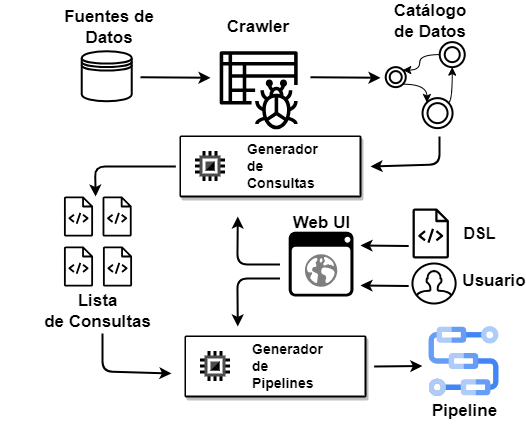
\includegraphics[width=0.60\textwidth]{Graphics/arch.drawio.png}
    \caption{Arquitectura del prototipo de AutoETL}
    \label{fig:arquitectura}
    \end{figure}

AutoETL se concibe como una herramienta para ser utilizada por los desarrolladores de almacenes de datos 
con el objetivo de aliviar la carga de trabajo en la implementaci\'on de los procesos de población de las 
estructuras analíticas. Como se observa en la Figura \ref{fig:arquitectura} los componentes de la aplicaci\'on 
est\'an dispuestos de forma secuencial para representar el flujo de trabajo de la herramienta.



\chapter{Implementación y Experimentos}\label{chapter:implementation}

Después de concebir y diseñar una solución computacional, es necesario llevar a cabo una implementación 
práctica para evaluar su validez. En este capítulo, se exponen las consideraciones fundamentales y 
las tecnologías empleadas en el desarrollo de un prototipo de la solución propuesta. Asimismo, se analiza 
la viabilidad del prototipo a través de la discusión de los resultados obtenidos en una serie de experimentos.


\section{Herramientas y tecnologías utilizadas}\label{section:tools}

\subsection{Lenguaje de programaci\'on Python}

Python\footnote{https://www.python.org} es un lenguaje de programación de alto nivel y propósito general que se caracteriza por ser 
interpretado, multi-paradigma, de tipado dinámico y con gestión automática de la memoria. Fue desarrollado 
por Guido Van Rossum en 1991 y en la actualidad se encuentra disponible en su versión 3.12.1.

La sintaxis de Python es conocida por ser simple e intuitiva, lo que facilita su accesibilidad tanto para 
investigadores, analistas como para programadores. Debido al crecimiento del uso de datos en las empresas y 
las facilidades que ofrece Python, el desarrollo del ecosistema profesional del lenguaje ha sido considerable. 
Actualmente, Python cuenta con múltiples bibliotecas y paquetes científicos que brindan diversas funcionalidades 
y son utilizados en varios campos de la ciencia e ingeniería.

En particular, existen bibliotecas especializadas en el trabajo con grafos, parsing, comunicación 
con sistemas de bases de datos, entre otras, que satisfacen las exigencias computacionales de la 
soluci\'on concebida. A continuación se reseñan las bibliotecas utilizadas para el desarrollo del prototipo.

\subsubsection{NetworkX}

NetworkX\footnote{https://networkx.org} es una biblioteca de Python diseñada para crear, manipular y analizar 
grafos y redes. Ofrece diversas 
opciones de estructuras de datos para representar grafos, incluyendo grafos no dirigidos, grafos dirigidos y 
multigrafos. La biblioteca proporciona una funcionalidad extensa para agregar atributos a los grafos, nodos y 
aristas, lo que la hace adaptable para una amplia gama de casos de uso. NetworkX se utiliza ampliamente para 
el estudio de redes complejas, lo que permite a los usuarios explorar la estructura, dinámica y funciones de 
los grafos. Es valioso para tareas como el análisis de redes, visualización de grafos y estudio de grandes 
redes complejas representadas en forma de grafos con nodos y aristas. En general, NetworkX sirve como una 
herramienta potente y popular para el análisis y manipulación de redes dentro del ecosistema de Python.

\subsubsection{PLY}

PLY\footnote{https://www.dabeaz.com/ply} es una implementación en Python de las 
herramientas de análisis léxico y sintáctico 
tradicionales lex y yacc. PLY utiliza el algoritmo de análisis LALR(1) y es 
compatible con todas las versiones modernas de Python. Es conocido por ser fácil de usar,
abarcar la mayoría de las características fundamentales de yacc y proporcionar una extensa verificación de errores. 
PLY permite la especificación de gramáticas 
mediante el uso de funciones de Python, lo que proporciona flexibilidad en la definición de la estructura del 
lenguaje a ser analizado. Esto implica la creación de funciones que representan las reglas de producción de la 
gramática, la definici\'on de los tokens y la especificación de las reglas de 
análisis como precedencia y asociatividad.

\subsubsection{Psycopg2}

Psycopg2\footnote{https://www.psycopg.org} es un adaptador ampliamente utilizado de base de datos PostgreSQL 
para el lenguaje de programación 
Python. Es reconocido por implementar completamente la especificación Python DB API 2.0 y ofrece un amplio 
soporte para interactuar con bases de datos PostgreSQL a través de Python. Esta biblioteca es conocida por 
su confiabilidad y su conjunto completo de funciones, lo que la convierte en la opción principal para muchos 
desarrolladores de Python que trabajan con PostgreSQL.

\subsubsection{Neo4j}

La biblioteca Neo4j\footnote{https://neo4j.com/} es el adaptador oficial para Python de bases de datos Neo4j. Está 
diseñada para proporcionar una 
interfaz de Python para ejecutar 
consultas y gestionar datos almacenados en dichas bases de datos en el contexto de aplicaciones de Python, lo que permite 
a los usuarios integrar y aprovechar las bondades de esta base de datos orientada a grafos directamente desde sus 
proyectos de Python.

\subsubsection{Streamlit}

Streamlit\footnote{https://streamlit.io} es una biblioteca de Python de código abierto que proporciona una forma rápida y sencilla para que los 
científicos de datos e ingenieros de aprendizaje automático conviertan los análisis de datos en aplicaciones web 
interactivas con un código mínimo. Está diseñado para simplificar el proceso de creación y despliegue de aplicaciones 
basadas en datos, optimizando flujos de trabajo que normalmente requieren un extenso desarrollo de la parte frontal. 
Las aplicaciones de Streamlit son scripts de Python mejorados con comandos específicos de Streamlit que luego se 
transforman en componentes de la interfaz de usuario. Este diseño 
permite una transición fluida de los scripts de datos a las aplicaciones web, con una curva de aprendizaje baja.


\subsection{PostgreSQL}

PostgreSQL\footnote{https://www.postgresql.org} es un sistema de gestión de bases de datos ampliamente utilizado y 
reconocido por sus sólidas 
características en la gestión y organización de datos. Es altamente valorado por su confiabilidad, escalabilidad, 
rendimiento, cumplimiento de ACID, compatibilidad con varios sistemas operativos y lenguajes de programación, lo que 
lo convierte en una opción popular para el desarrollo de una amplia gama de aplicaciones 
como aplicaciones web, 
almacenes de datos y procesamiento de grandes volúmenes de datos. 
Al ser un sistema de gesti\'on de bases de datos de código abierto, PostgreSQL es rentable y se beneficia del 
desarrollo continuo impulsado por la comunidad, actualizaciones oportunas y una amplia documentación y recursos 
disponibles.

\subsection{Neo4j}

\subsection{Docker}
\section{Implementación del prototipo}\label{section:prototype}

El prototipo implementado se concibe como una aplicación web. Se compone de cuatro componentes: crawler, catálogo de datos, generador de consultas 
e interfaz de usuario; los cuales se corresponden con la concepción y el diseño del sistema propuesto en el capítulo \ref{chapter:proposal}, 
ilustrado en la figura \ref{fig:arquitectura}. 
La lógica de los análisis sintáctico y léxico del lenguaje de dominio específico, DSL, propuesto fue incluida como parte 
del generador de consultas. 

Por cuestiones de tiempo no se pudo concretar una implementación del generador de pipelines. 
La implementación de este componente plantea desafíos considerables. Primeramente, 
este debe ser independiente de los sistemas gestores de bases de datos de la fuente y del almacén de datos. 
Además, su implementación implica la implementación de la lógica para los tipos de extracción y carga de datos. 
Por otro lado, el generador de pipelines también es el encargado de ejecutar los pipelines de forma autónoma, 
por tanto se debe implementar un mecanismo de captura de eventos que dictamine en que momento ejecutar el pipeline.

Durante el proceso de investigación previo a la implementación se identificó que con la utilización de la  
plataforma Apache Airflow\footnote{https://airflow.apache.org} se pueden satisfacer varios de los 
requisitos funcionales del generador de pipelines. Airflow es una herramienta de orquestación de flujos de 
trabajo de procesamiento de datos que permite a los desarrolladores definir y monitorear flujos de trabajo. 
Un flujo de trabajo es modelado como un grafo dirigido y ac\'iclico, (DAG), cuyos nodos representan tareas y los 
arcos modelan la dependencia entre las tareas. Los DAG son definidos mediante scripts de Python, en los cuales 
se especifican las tareas a realizar mediante operadores de Airflow y su \'orden. Luego, generar un DAG 
cuyas tareas sean la ejecución de las consultas construidas por el generador de consultas para la población de 
un escenario analítico determinado implica generar 
din\'amicamente un script de Python que de definición al DAG. Además, la estructura de dicho script 
no es estática pues el n\'umero de tareas a realizar y su orden dependen del escenario analítico a poblar,
y los operadores de Airflow para la ejecución de las consultas varían según el sistema gestor de base de 
datos de la fuente y del sistema destino. Por tanto, la generación dinámica del script de python que define un DAG 
no es un proceso trivial.

Luego, la implementación del generador de pipelines mediante el uso de Airflow plantea desafíos significativos que 
no pudieron ser resueltos debido al alto volumen de trabajo necesario para implementar otros componentes del marco 
de trabajo propuesto y al tiempo disponible para la realización de esta investigación. Por lo tanto, se propone 
la implementación del generador de pipelines como trabajo futuro.

\subsection{Organización de los archivos}

La lógica de cada uno de los componentes de la aplicación se encuentra separada por carpetas. Cada componente 
posee su propia carpeta identificada con el nombre del componente en inglés, a excepción de la interfaz de usuario 
cuya carpeta es nombrada \textbf{pages} y su script principal se encuentra en la raíz del proyecto con el nombre de 
\textbf{MainPage.py}. Todos los datos derivados de la ejecución de la lógica de cada uno de los componentes 
se almacena dentro de la carpeta \textbf{data}. La carpeta \textbf{utils} guarda scripts de algoritmos usados 
en varias partes de la aplicación, concretamente posee scripts con algoritmos para la carga y escritura de los 
grafos y \'arboles de join en el disco.

\subsection{Fuentes de datos}

El prototipo maneja una única fuente de datos a la vez, aunque es posible considerar varias 
fuentes de datos para un mismo almacén de datos de destino. Para esto se debe definir un script del DSL por 
cada fuente de datos que alimente el almacén de datos. Las primeras consultas de creación generadas que se ejecuten 
para dicho almacén determinarán el nombre de las tablas de las dimensiones y de los hechos, as\'i como 
como el nombre de sus atributos, sus tipos y restricciones. Luego, para alimentar el almacén de datos con otras 
fuentes, basta con ejecutar las consultas de selección generadas a partir del script correspondiente a 
dicha fuente y, con posterioridad, insertar en el almacén los valores extra\'idos.

\subsection{Crawler}

El Crawler constituye un elemento de interdependencia dentro del prototipo en relación con los sistemas 
que administran las fuentes de datos, específicamente con los los sistemas de gestión de bases de datos, (SGBD). 
Con el objetivo de lograr una 
mayor extensibilidad, se plantea la creación de una clase abstracta llamada \textbf{crawler}, la cual establecerá 
el comportamiento general de este componente. De este modo, se delega a las implementaciones específicas para cada 
SGBD la definición de la forma en que se llevan a cabo las operaciones, como se muestra en la figura \ref{fig:crawler}. 
El ejemplo de código \ref{code:crawler} muestra la definición de la clase abstracta \textbf{crawler}.

\begin{figure}[H]
    \centering
    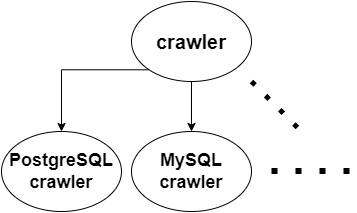
\includegraphics[width=0.5\textwidth]{Graphics/crawler_class.drawio.png}
    \caption{Jerarquía de la clase abstracta crawler}
    \label{fig:crawler}
\end{figure}

\begin{lstlisting}[label={code:crawler}, caption={Definición de la clase abstracta crawler}, language={python}]
    import abc

    class Crawler(metaclass=abc.ABCMeta):
        def __init__(self, dbname, user, password, host, port) -> None:
            self.dbname = dbname
            self.user = user
            self.password = password
            self.host = host
            self.port = port
            self._db_params = {'dbname': dbname, 'user': user, 'password': password, 'host': host, 'port': port}
            self._metadata_str = ''
            self._db_dict = {}

        @abc.abstractmethod
        def explore_db(self):
            pass
        
        @abc.abstractmethod
        def export_metadata_to_file(self):
            pass

\end{lstlisting}

La implementación de esta clase se encuentra en el archivo \textbf{crawler.py} de la carpeta del componente homónimo. Los 
campos de la clase se corresponden con la información necesaria para establecer una conexión con una base de 
datos. 

El método \textbf{explore\_db} se encarga de recopilar los metadatos de la fuente de datos con nombre \textbf{dbname}. 
Los metadatos recopilados son, como ya se mencion\'o en el cap\'itulo de concepción y diseño, los nombres de las 
tablas de la base de datos fuente, por cada tabla se obtienen sus
atributos, por cada atributo su tipo y si son llaves primarias. Además, por cada tabla
se obtienen los atributos que son llaves foráneas y, por cada una, se extrae el nombre
de la tabla a la que referencian y el atributo referenciado. Los metadatos recopilados se almacenan en el diccionario 
\textbf{\_db\_dict}, el cual tiene como llaves los nombres de las tablas de la base 
de datos y como valores otros diccionarios que poseen dos llaves: \textbf{attributes} y \textbf{relations}. 
El valor de \textbf{attributes} es una lista de tuplas de dos o tres elementos, una por cada atributo de la tabla. 
Las tuplas de dos elementos almacenan el nombre del atributo y el tipo, las de tres almacenan además un indicador 
que expresa si el atributo es llave primaria, for\'anea o ambas. El valor de \textbf{relations} es una lista de 
tuplas de tres elementos, una por cada atributo que es una llave foránea de la tabla. El primer elemento es el nombre 
de la llave for\'anea en la tabla, el segundo el nombre de la tabla referenciada y el tercero el atributo referenciado. 
El ejemplo de c\'odigo \ref{dbdict} muestra la estructura del diccionario \textbf{\_db\_dict}. 

\begin{lstlisting}[label={dbdict}, caption={Estructura del diccionario \textbf{\_db\_dict}}]
_db_dict: {
    'tabla_1' : {
        attributes: [(atr_1, tipo, PK FK), ..., (atr_n, type)]
        relations: [(atr_1, tabla_ref, atr_ref), ...]
    }
    .
    .
    .
    'tabla_n': { ... }
}
\end{lstlisting}

Además, el método \textbf{explore\_db} tiene la responsabilidad de llenar la cadena de texto \textbf{\_metadata\_str} 
que almacena los metadatos recopilados en un formato m\'as expresivo para luego ser mostrado al desarrollador.

El método \textbf{export\_metadata\_to\_file} se encarga de guardar \textbf{\_db\_dict} y \textbf{\_metadata\_str} en el disco, 
en la ruta \textbf{data/schemas}. La carpeta \textbf{schemas} contiene una carpeta por cada base de datos, identificada 
por el nombre de la base de datos, en la cual se almacena \textbf{\_db\_dict} en formato json y 
\textbf{\_metadata\_str} en formato txt.

En esta primera entrega del prototipo solo se implement\'o un crawler para PostgreSQL. Su l\'ogica 
se encuentra en el archivo \textbf{postgreSQL\_crawler.py}. Los metadatos son recopilados mediante consultas 
realizadas
a la tabla \textbf{information\_schema} de la base de datos fuente, utilizando para la ejecución de las consultas 
el adaptador de PostgreSQL para python \textbf{psycopg2}.




\subsection{Catálogo de Datos}

El catálogo de datos es un servidor de bases de datos de Neo4j que contiene un grafo por cada base de datos 
fuente que haya sido explorada por la aplicación. Cada vez que el crawler explora una base de datos fuente nueva se crea 
un grafo de base de datos de Neo4j para almacenar sus metadatos.

La comunicación de la aplicación con el Catálogo de Datos es mediada por la clase \textbf{DataCatalogHandler} 
presente en el script \textbf{handler.py} de la carpeta \textbf{data\_catalog}. En el ejemplo de c\'odigo 
\ref{code:catalog} se muestra parte del código de dicha clase.

\begin{lstlisting}[label={code:catalog}, caption={Clase DataCatalogHandler}, language={python}]
    class DataCatalogHandler():
        def __init__(self, db_dict, db_name, user, password, uri) -> None:
            self.db_dict = db_dict
            self._user = user
            self._password = password
            self._uri = uri
            self.db_name = db_name
            self.join_graph = None

        def create_database(self):
            # Omitted implementation

        def populate_graph_database(self):
            # Omitted implementation

        def export_join_graph(self):
            # Omitted implementation

\end{lstlisting}

El campo \textbf{db\_dict} hace referencia al diccionario de la base de datos confeccionado por el crawler, ver ejemplo de c\'odigo \ref{dbdict}, 
\textbf{db\_name} almacena el  
nombre de la base de datos fuente, \textbf{join\_graph} almacena una referencia en memoria del grafo de joins construido 
durante la ejecución de \textbf{export\_join\_graph}. El resto de atributos 
son los necesarios para establecer una conexión con una base de datos de Neo4j; en especial, el campo \textbf{\_uri} 
es una cadena de texto que contiene el protocolo de comunicación con el servidor de Neo4j, su ip y su puerto. 

El método \textbf{create\_database} crea una base de datos de Neo4j en el catálogo de datos dedicada a la 
fuente de datos con nombre \textbf{db\_name} y con diccionario de metadatos \textbf{db\_dict}. 

El método \textbf{populate\_graph\_database} se encarga de poblar la base de datos de Neo4j con los metadatos
recopilados. Se crea 
un nodo por cada llave 
de \textbf{db\_dict} con las propiedades \textbf{name} que almacena el nombre de la tabla, \textbf{pks} que es una 
lista con los nombres de los atributos que son llaves primarias y, por \'ultimo, \textbf{attributes} que 
es la lista de tuplas correspondiente a la llave attributes del diccionario que devuelve \textbf{db\_dict} como valor
al ser indexado  en el nombre de la tabla en cuestión (\textbf{db\_dict[table\_name]}). Además, se crea una relación direccionada por cada llave for\'anea 
presente en la lista correspondiente a la llave relations del diccionario que devuelve \textbf{db\_dict} 
como valor al ser indexado en el nombre de la tabla en cuestión. La dirección de la relación lo dictamina 
el sentido de la referencia de la llave 
for\'anea, tal y como se expuso en el capitulo \ref{chapter:proposal} en la sección referente al catálogo de 
datos.

El método \textbf{export\_join\_graph} es el encargado de construir, a partir de la base de datos Neo4j del esquema 
de la fuente de turno, el grafo de joins. Mediante el lenguaje de consulta Cypher y el adaptador de Neo4j para Python 
se extraen todos los nodos y relaciones y se crea un digrafo de NetworkX equivalente, que además conserva las 
propiedades definidas para nodos y relaciones. Este digrafo es el grafo de joins. Se le añaden arcos 
adicionales siguiendo la teoría expuesta para el grafo de join en el capitulo \ref{chapter:proposal} en la 
sección del generador de consultas, específicamente en el ac\'apite referido a la inferencia de joins. 
Luego 
de creado el grafo de join se almacena en la ruta \textbf{data/join\_graphs} con el nombre de la base de datos fuente 
a que corresponde. La figura \ref{fig:schema-catalog} y la figura \ref{fig:catalog-jgraph} muestran, seg\'un lo 
explicado con anterioridad, la 
transici\'on de un esquema de bases de datos a un grafo del cat\'alogo de datos y la 
transición de un grafo del cat\'alogo de datos a un grafo de joins respectivamente. 

\begin{figure}[H]
    \centering
    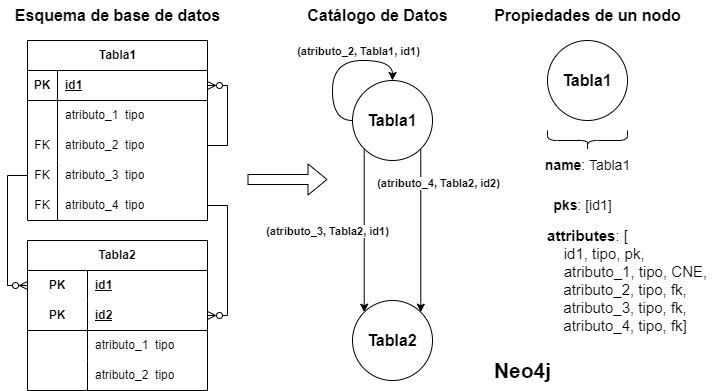
\includegraphics[width=0.7\textwidth]{Graphics/schema-catalog.drawio.png}
    \caption{Transición del esquema de bases de datos al cat\'alogo de datos}
    \label{fig:schema-catalog}
\end{figure}

La propiedad \textbf{attributes} en un nodo de un grafo del catálogo es una lista aplanada de los metadatos 
pues Neo4j no admite estructuras complejas 
como las listas de tuplas. Las siglas \textbf{CNE} significan \emph{constraint not specified} 
e indica que el atributo cuyo nombre se encuentra dos posiciones antes no es llave primaria o 
llave for\'anea. Cuando se construye el grafo de joins a partir del grafo del catálogo se retoma 
la estructura de lista de tuplas para la propiedad \textbf{attributes} como muestra la figura 
\ref{fig:catalog-jgraph}

\begin{figure}[H]
    \centering
    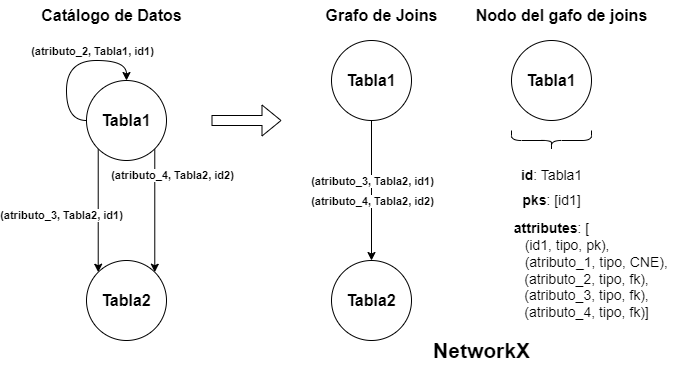
\includegraphics[width=0.7\textwidth]{Graphics/catalog-jgraph.drawio.png}
    \caption{Transición del catálogo de datos al grafo de joins}
    \label{fig:catalog-jgraph}
\end{figure}

\subsection{Generador de Consultas}

La implementación concebida para el generador de consultas est\'a compuesta por las implementaciones para el tratamiento de los scripts del lenguaje de 
dominio específico y generación de consultas, y por las implementaciones referentes a la construcci\'on 
y consulta de los \'arboles de join para la inferencia de joins.



\subsubsection{Lenguaje de Dominio Espec\'ifico}

La lógica del DSL se encuentra en la ruta \textbf{query\_generator/dsl}. El uso de la biblioteca 
PLY demanda la creación de dos scripts, uno donde se especifiquen los terminales de la gramática y las reglas 
para el análisis léxico y, otro, donde se especifiquen las producciones de la gramática mediante funciones. Estos 
scripts son \textbf{lexer.py} y \textbf{parser\_rules.py} respectivamente. En el script \textbf{ast\_nodes.py} se define  
la jerarquía de clases de los nodos del \'arbol de sintaxis abstracta (AST) del lenguaje de dominio específico expuesto 
en el capítulo \ref{chapter:proposal} y cuya gramática libre del contexto puede encontrarse en el ejemplo de 
c\'odigo \ref{code:CFG}. Cada 
estructura gramatical del lenguaje est\'a representada por una clase, como se muestra en la figura \ref{fig:ast}.

\begin{figure}[htb]
    \centering
    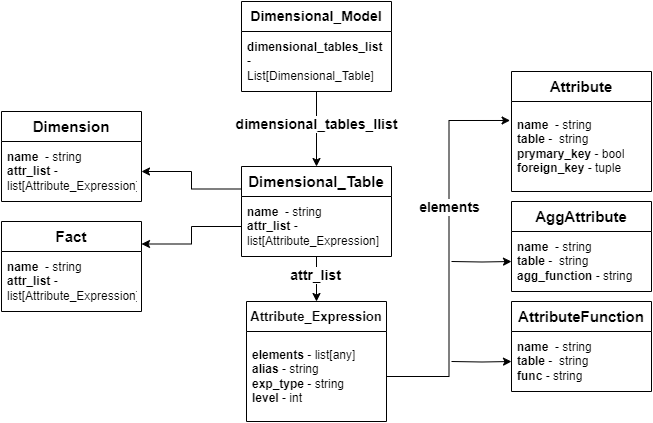
\includegraphics[width=0.7\textwidth]{Graphics/ast.png}
    \caption{Estructura del AST}
    \label{fig:ast}
\end{figure}

La clase \textbf{Dimensional\_Schema} representa un esquema dimensional en forma de estrella, el cual est\'a formado por una lista de tablas 
dimensionales \textbf{Dimensional\_Table}. Las clases \textbf{Dimension} y \textbf{Fact} heredan de \textbf{Dimensional\_Table} 
y representan a las dimensiones y a las tablas de hechos respectivamente. La clase \textbf{Attribute\_Expression} expresa 
la definición de un atributo, ya sea simple o una expresión aritmética donde participen varios atributos y n\'umeros. 
Las clases \textbf{Attribute}, \textbf{AggAttribute} y \textbf{AttributeFunction} representan atributos simples, atributos 
agregados y atributos resultado de la aplicación de alguna función respectivamente. El campo \textbf{foreign\_key} de 
la clase \textbf{Attribute}, en caso de tener alg\'un valor almacenado, es una tupla que indica que la instancia 
de \textbf{Attribute} es una llave for\'anea y en la primera posición de la tupla se almacena el nombre de la tabla referenciada y 
en la segunda posición, el nombre del atributo referenciado.

Una instancia de \textbf{Dimensional\_Schema} contiene una lista de instancias de \textbf{Dimensional\_Table}, las que a su vez pueden ser de tipo 
\textbf{Dimension} o \textbf{Fact}. Las instancias de \textbf{Dimension} o \textbf{Fact} poseen una lista de instancias de \textbf{Attribute\_Expression}, cada 
una de ellas presenta 
una lista llamada \textbf{elements} que puede contener uno o varios elementos; en caso de tener uno solo, el elemento 
es una instancia de \textbf{Attribute}, \textbf{AggAttribute} o \textbf{AttributeFunction}. En caso de tener 
m\'as de un elemento, es decir, la instancia de \textbf{Attribute\_Expression} representa un atributo compuesto, entonces 
\textbf{elements} contiene tanto las instancias de \textbf{Attribute}, \textbf{AggAttribute} o \textbf{AttributeFunction} como 
los signos de agrupación y operadores que participan en la definición del atributo.

Los scripts del DSL son tokenizados con la instancia de lexer declarada en \textbf{lexer.py}. La lista de tokens 
resultante pasa a ser analizada por la instancia de parser declarada en \textbf{parser\_rules.py}. El resultado 
del análisis sintáctico del parser es el \'arbol de sintaxis abstracta del script del DSL analizado.


\subsubsection{Generaci\'on de c\'odigo}

Luego de tener construido el árbol de sintaxis abstracta, AST, del script específico se pasa a realizar un análisis sobre 
esta estructura con 
el objetivo de detectar errores semánticos en el código del script. Si no se encuentran errores, 
a partir del AST se comienza a generar el código de las consultas de creación y selección.

Siguiendo las mejores prácticas de la industria, todos los análisis sobre el AST se realizan 
utilizando el patrón visitor\cite{buttner2004digging}. Cada nodo del AST implementa la clase abstracta 
\textbf{Visitable} presente en \textbf{visitable.py}. El ejemplo de c\'odigo \ref{code:visitable} 
muestra el c\'odigo de la clase \textbf{Visitable}.

\begin{lstlisting}[label={code:visitable}, caption={Clase abstracta Visitable}, language={python}]
    import abc

    class Visitable(metaclass = abc.ABCMeta):
        @abc.abstractmethod
        def accept(self, visitor):
            pass
\end{lstlisting}

Por tanto, todo nodo del AST posee un método \textbf{accept} que recibe un visitor específico. La implementación 
puntual de \textbf{accept} para cada tipo de nodo del AST consiste en llamar al método \textbf{visit}, del visitor pasado como argumento, 
que le corresponde a su tipo. Los visitors implementados pueden encontrarse en el script \textbf{visitors.py} y la 
figura \ref{fig:visitors} muestra la jerarquía de clases de los visitors implementados.

\begin{figure}[htb]
    \centering
    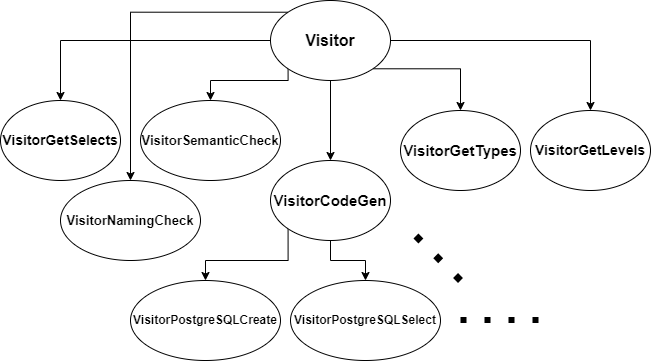
\includegraphics[width=0.7\textwidth]{Graphics/visitorfixed.drawio.png}
    \caption{Jerarquía de Visitors}
    \label{fig:visitors}
\end{figure}

La clase \textbf{Visitor} es la raíz de la jerarquía. Es una clase abstracta en la que se definen los métodos 
\textbf{visit} que deben tener todas las clases herederas. En particular, hay un \textbf{visit} por cada tipo de 
nodo del AST, lo que se detalla en el ejemplo de c\'odigo \ref{code:visitors}

\begin{lstlisting}[label={code:visitors}, caption={Clase Visitor}, language={python}]
    class Visitor(metaclass = abc.ABCMeta):
        @abc.abstractmethod
        def visit_dimensional_schema(self, dimensional_model): pass 

        @abc.abstractmethod
        def visit_attribute(self, attribute): pass

        @abc.abstractmethod
        def visit_attr_function(self, attr_func): pass

        @abc.abstractmethod
        def visit_agg_attr(self, agg_attr): pass

        @abc.abstractmethod
        def visit_attr_expression(self, attr_expression): pass

        @abc.abstractmethod
        def visit_dimensional_table(self, dimensional_table): pass
\end{lstlisting}

Las instancias de las clases \textbf{VisitorSemanticCheck}, \textbf{VisitorNamingCheck}, \textbf{VisitorGetTypes} 
son las encargadas de realizar
controles semánticos sobre el código del script del DSL analizado. Las instancias de \textbf{VisitorSemanticCheck} realizan los siguientes 
chequeos:

\begin{itemize}
    \item Revisan si en el esquema estrella definido existe al menos una dimensión y una tabla de hechos.
    \item Se aseguran que las tablas definidas tengan al menos un atributo válido.
    \item Se aseguran que todas las tablas tengan definidas al menos una llave primaria.
    \item Verifican que no existan llaves for\'aneas declaradas en atributos compuestos.
    \item Verifican que tanto los atributos referenciados como las tablas referenciadas est\'en definidos en el 
        script.
    \item Revisan si las tablas y los atributos fuente utilizados en el script existen en la base de datos fuente.
    \item Verifican el correcto uso de la palabra reservada \textbf{self}.
\end{itemize}

Las instancias de \textbf{VisitorNamingCheck} se encargan de recorrer el AST y verificar que: 

\begin{itemize}
    \item En las dimensiones o tablas de hechos no existan dos atributos definidos con el mismo nombre.
    \item No existan dos tablas del esquema estrella con el mismo nombre.
    \item Los atributos compuestos definidos tengan asignados un alias para su correcta identificación.
\end{itemize}

Las instancias de \textbf{VisitorGetTypes} son las responsables de verificar el buen uso de los tipos en el 
código del DSL además de recolectar el tipo de cada atributo declarado en cada dimensión y 
en la tabla de hechos, 
información necesaria para el proceso de generación de código. En particular, realizan 
las siguientes verificaciones: 

\begin{itemize}
    \item Verifican que los atributos compuestos definidos se les haya especificado su tipo.
    \item En el caso de las llaves for\'aneas comprueban que la llave for\'anea y el atributo referenciado 
        coincidan en tipo.
\end{itemize}

Las instancias de \textbf{VisitorGetSelects} se encargan de recorrer el AST y por cada tabla dimensión o tabla 
de hechos recolectan las tablas y los atributos que hay que seleccionar de la fuente de datos 
para poblar las tablas respectivas. A partir de esta información se confeccionan las consultas 
que se realizan a los \'arboles de join para obtener el join necesario para el proceso de población.

Las instancias de \textbf{VisitorGetLevel} son las encargadas de recopilar los niveles de cada uno de los 
atributos de las tablas del esquema estrella. Esta información luego se exportar\'a al almacén de datos 
destino en forma de una tabla de metadatos llamada \textbf{level\_metadata}. Dicha tabla tendrá tres atributos: 
\textbf{table\_name}, \textbf{attribute\_name} y \textbf{level}. El primero es el nombre de la tabla del esquema 
estrella, el segundo es el nombre del atributo y el tercero es un entero que representa el nivel del atributo 
en la jerarquía de la tabla con nombre \textbf{table\_name}.

La clase \textbf{VisitorCodeGen} es una clase abstracta de la que heredar\'an todos los visitors que 
se encarguen de generar código. Hereda de la clase \textbf{Visitor} y la extiende pues incorpora un 
método para exportar las consultas generadas, como se muestra en el ejemplo de c\'odigo \ref{code:vcodegen}.

\begin{lstlisting}[label={code:vcodegen}, caption={Clase VisitorCodeGen}, language={python}]
    class VisitorCodeGen(Visitor):
        def visit_dimensional_model(self, dimensional_model):
            return super().visit_dimensional_model(dimensional_model)
        def visit_dimensional_table(self, dimensional_table):
            return super().visit_dimensional_table(dimensional_table)
        def visit_attr_expression(self, attr_expression):
            return super().visit_attr_expression(attr_expression)
        def visit_attribute(self, attribute):
            return super().visit_attribute(attribute)
        def visit_attr_function(self, attr_func):
            return super().visit_attr_function(attr_func)
        def visit_agg_attr(self, agg_attr):
            return super().visit_agg_attr(agg_attr)

        @abc.abstractmethod
        def export_querys(self): pass
\end{lstlisting}

La generación de código es otro de los puntos de dependencia del prototipo con los sistemas de gestión 
de bases de datos. Específicamente, las consultas de selección dependen del sistema de gestión de bases 
de datos de la fuente, pues estas se encargan de extraer los datos para la población, y las consultas 
de creación dependen del sistema de gestión de bases de datos del almacén de datos de destino, pues 
son las responsables de crear las tablas del esquema estrella. Para resolver esta dependencia 
se implementa un visitor para la generación de las consultas de selección y un visitor para la generación 
de las consultas de creación, por cada sistema de gestión de bases de datos, como se muestra en la 
figura \ref{fig:visitors}. De esta forma, cada tipo de consulta la genera el visitor que le corresponde 
al sistema de gestión de bases de datos de la fuente o del destino. En esta primera versión del prototipo 
se implementaron los visitors de generación de código para PostgreSQL.

Las instancias de la clase \textbf{VisitorPostgreSQLCreate} son las encargadas de generar las 
consultas de creación de las tablas del esquema estrella para el sistema gestor PostgreSQL. En la 
declaración de los atributos 
dentro de la consulta se utiliza la información recolectada por \textbf{VisitorGetTypes} para 
especificar los tipos de los atributos que se crear\'an. Pero las instancias de \textbf{VisitorGetTypes} 
recolectan los tipos que maneja el DSL, por tanto, cada instancia de \textbf{VisitorPostgreSQLCreate} 
tiene un diccionario que mapea los tipos del DSL a los tipos de PostgreSQL.

Las instancias de la clase \textbf{VisitorPostgreSQLSelect} generan las consultas de selección para 
el sistema gestor PostgreSQL. Reciben los joins seleccionados por el desarrollador para cada tabla del esquema 
estrella y conforman las consultas de selección.

\subsubsection{Inferencia de joins}

La implemetaci\'on de la l\'ogica para la inferencia de joins se encuentra repartida 
en los scripts de Python \textbf{maximal\_join\_trees.py}, \textbf{join\_computation.py} y 
\textbf{all\_spanning\_trees.py}. 

A modo de recordatorio, en el cap\'itulo de concepción y diseño se expuso que los \'arboles de expansión 
de los grafos alcanzables originados desde nodos del grafo de join con indegree cero, o pertenecientes 
a una componente fuertemente conexa sin arcos incidentes exteriores, constituyen el conjunto de \'arboles 
de join a partir de los cuales se realizar\'a la inferencia de joins.

En script \textbf{all\_spanning\_trees.py} yacen los algoritmos para la obtención de los \'arboles de expansión 
de un grafo alcanzable, como se muestra en el ejemplo de c\'odigo \ref{code:stgen}.

\begin{lstlisting}[label={code:stgen}, caption={Algoritmo para la generación de \'arboles de expansión}, language={python}]
    def networkX_all_spanning_trees(graph:DiGraph) -> list[DiGraph]:
        result = []
        for tree in ArborescenceIterator(graph):
            result.append(tree)

        return result
\end{lstlisting}

En esta primera entrega solo se implement\'o una variante que se apoya en la 
clase ArborescenceIterator de NetworkX, la cual constituye un iterador de los \'arboles de expansión de un digrafo 
pasado como argumento.


En el script \textbf{maximal\_join\_trees.py} yace
la implementación en Python del pseudoc\'odigo propuesto para la fase de precomputaci\'on, en el 
capítulo \ref{chapter:proposal} en la sección del generador de consultas, específicamente en el ac\'apite referido 
a la inferencia de joins, ver ejemplo de c\'odigo \ref{precom}. El m\'etodo \textbf{maximal\_join\_trees\_generator} 
constituye la implementación del pseudoc\'odigo de la fase de precomputaci\'on y toma como argumentos 
un grafo de joins y devuelve una lista de \'arboles de join. Los \'arboles de join también son digrafos de 
NetworkX con las mismas propiedades definidas para los nodos y arcos que presenta el grafo de joins, 
ilustradas en la figura \ref{fig:catalog-jgraph}.

Para la generación de los \'arboles de join, \textbf{maximal\_join\_trees\_generator} se apoya en 
el m\'etodo \textbf{\_find\_reachable} para calcular el grafo alcanzable desde un nodo ra\'iz en el grafo 
de joins y del m\'etodo \textbf{\_in\_edge\_from\_outside} para verificar si una componente fuertemente 
conexa posee arcos incidentes desde el exterior. Las componentes fuertemente conexas son calculadas 
utilizando el m\'etodo \textbf{strongly\_connected\_components} de la biblioteca NetworkX. A los nodos 
de los \'arboles generados se les añade, mediante el método \textbf{\_set\_height}, la propiedad \textbf{height} que almacena 
la altura del nodo con respecto a la raíz del \'arbol, con el objetivo de facilitar el c\'omputo 
del ancestro com\'un m\'as bajo de un conjunto de nodos. Por \'ultimo, 
los árboles de join son almacenados en la ruta \textbf{data/join\_trees}.


El script \textbf{join\_computation.py} alberga el m\'etodo \textbf{compute\_joins}, el cual es la implementación 
en Python del algoritmo \textbf{get\_joins} cuyo pseudoc\'odigo fue expuesto en el capítulo \ref{chapter:proposal} 
en el ejemplo de c\'odigo \ref{querytime}. El ejemplo de c\'odigo \ref{computejoins} muestra el c\'odigo del 
m\'etodo \textbf{compute\_joins}.

\begin{lstlisting}[label={computejoins}, caption={C\'odigo del m\'etodo \textbf{compute\_joins}}, language={python}]
    def compute_joins(join_trees: list[DiGraph], tables_list) -> str:
        valid_join_trees = _get_answer_trees(join_trees, tables_list)
        all_joins = []
        for tree in valid_join_trees:
            lca = _lowest_common_ancestor(tree, tables_list)
            join = _get_join(tree, lca, tables_list)
            if join not in all_joins:
                all_joins.append(join)

        return all_joins
\end{lstlisting}

Este algoritmo recibe la lista de \'arboles de joins generados y una 
lista de tablas a concatenar y devuelve una lista de joins. La lista de tablas a concatenar es provista por el 
visitor \textbf{VisitorGetSelects}. El m\'etodo \textbf{\_get\_answer\_trees} dado una lista de 
\'arboles de join y una lista de tablas a concatenar devuelve los \'arboles de join que contienen todas las tablas de 
la consulta, representada en la lista \textbf{tables\_list}, y por tanto pueden proporcionar interpretaciones 
para la consulta. El m\'etodo \textbf{\_lowest\_common\_acestor} calcula el ancestro com\'un m\'as bajo, LCA, para el 
conjunto de tablas en \textbf{tables\_list}. El m\'etodo \textbf{\_get\_join} construye el subárbol del \'arbol 
de join \textbf{tree}, que constituye una interpretaci\'on de la consulta para dicho \'arbol de join, y lo 
convierte en una lista que representa una secuencia de joins para facilitar el proceso de generación del c\'odigo del join computado. 
Los componentes de la lista que representa una secuencia de joins se alternan entre el nombre de las tablas 
y una lista con tuplas que representan las condiciones del join entre las tablas. El ejemplo de c\'odigo \ref{joinlist}
ilustra la estructura de la lista que representa una secuencia de joins.

\begin{lstlisting}[label={joinlist}, caption={Estructura de una lista que representa una secuencia de joins}, language=python]
    ['tabla1', [('tabla1.atr1', 'tabla2.atr2'), ...], 'tabla2', ...]
\end{lstlisting}

La lista del ejemplo de c\'odigo \ref{joinlist} representa el join entre las tablas \textbf{tabla1} y \textbf{tabla2} 
bajo la condición (\textbf{tabla1.atr1 = tabla2.atr2 and ...}). Por supuesto, la secuencia de joins 
que representa una lista con esta estructura no est\'a limitada a un join entre solo dos tablas.

N\'otese que como los \'arboles de join comparten las propiedades del grafo de joins, mediante un recorrido 
DFS sobre el subárbol que representa una interpretaci\'on de una consulta sobre un \'arbol de join determinado, se puede 
obtener una lista con la estructura que se muestra en el ejemplo de c\'odigo \ref{joinlist}. 

La figura \ref{fig:allpro} muestra como interactúan los componentes anteriormente explicados 
para obtener, a partir de la definición de un escenario anal\'itico, las consultas de creación y las consultas de  
selección.

\begin{figure}[H]
    \centering
    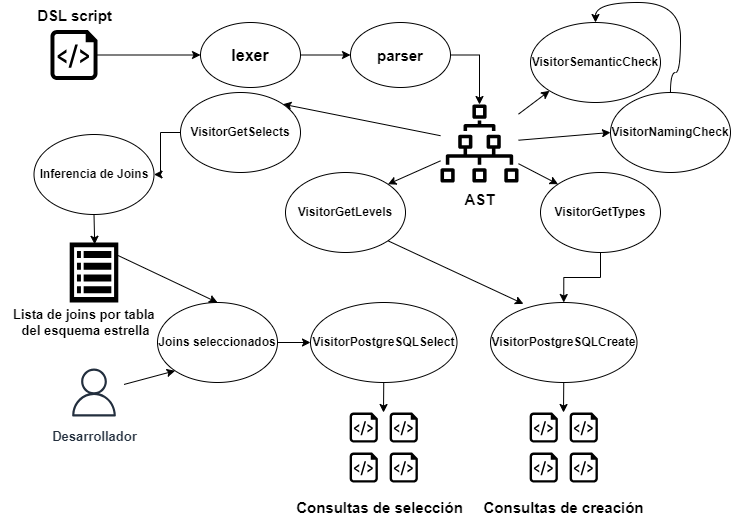
\includegraphics[width=0.7\textwidth]{Graphics/all_procces.drawio.png}
    \caption{Proceso de generación de consultas desde el inicio.}
    \label{fig:allpro}
\end{figure}

\subsection{Interfaz de Usuario}

Para la implementación de la interfaz de usuario se utilizó la biblioteca Streamlit de Python. Esta biblioteca 
permite la implementación de aplicaciones web mediante la definición de scripts de Python donde se 
definan los componentes de las páginas de la aplicación mediante la API de Streamlit. Además, proporciona un 
servidor para alojar la aplicación e interactuar con ella. La interfaz de usuario de la aplicación cuenta 
con cuatro páginas. La página principal se define en el directorio raíz de la aplicación y el resto de las 
páginas dentro de una carpeta llamada \textbf{pages}. 

\subsubsection{Main Page}

Esta es la página principal de la aplicación, cuya imagen se muestra en la figura \ref{fig:mainpage} como anexo. 
En el script \textbf{Main\_Page.py} se definen 
los componentes de la página. En Main Page el desarrollador deber\'a establecer la conexión con un servidor de 
bases de datos fuente y escoger si desea realizar un proceso de recomputaci\'on de la conexión. El 
proceso de recomputaci\'on consiste en crear una instancia de crawler para explorar la base de datos 
fuente, crear la base de datos de Neo4j correspondiente al esquema de la fuente de datos en el catálogo 
de datos y exportar el grafo de join y los \'arboles de join derivados. Como se expuso en el capítulo 
\ref{chapter:proposal} este cómputo es costoso, por tanto solo est\'a pensado para realizarse la primera 
vez que se descubre la base de datos fuente o cuando el esquema de la misma sufra cambios. En este \'ultimo caso, 
el catálogo de datos, el grafo de join y los \'arboles de join serían inválidos y necesitan ser recalculados. 
Además, la página cuenta con un formulario para registrar nuevos servidores de bases de datos. La información 
de los servidores es almacenada en la ruta \textbf{data/connections} en formato json.

\subsubsection{Metadata}

En esta página se muestran los metadatos recopilados por el crawler, as\'i como las imágenes del 
grafo de join y los \'arboles de join derivados. El script de esta página es \textbf{Metadata.py} y 
la imagen se muestra en la figura \ref{fig:meta} como anexo.

\subsubsection{Query Generator}

En esta página se muestran las consultas generadas. Como anexos se incluyen la imagen de la página 
Query Generator en la figura \ref{fig:generator}, así como fragmentos de consultas generadas en 
la figura \ref{fig:qfragment}.
Primero se selecciona un script del DSL que 
define un esquema estrella a poblar. Luego se debe escoger, por cada tabla del esquema estrella, el 
join que mejor se ajuste para la extracción de los valores. La selección se realiza a través 
de componentes en la interfaz de usuario. Una vez seleccionados los joins, aparecer\'a un bot\'on 
para comenzar el proceso de generación de las consultas  
de creación y de selección para cada tabla del esquema estrella, as\'i como la consulta 
para crear y poblar la tabla de metadatos \textbf{level\_metadata}. Las consultas generadas 
son almacenadas en la ruta \textbf{data/querys}, lo que posibilita su recuperación y descarga por parte del desarrollador. 
Todo el proceso de generación y análisis del script del DSL es mediado por la clase \textbf{Orchestrator}, 
presente en \textbf{orchestrator.py}, como se muestra en el ejemplo de c\'odigo \ref{code:orchestrator}.

\begin{lstlisting}[label={code:orchestrator}, caption={Clase Orchestrator}, language={python}]
    class Orchestrator:
        def __init__(self, dbname, dwname, source_sgbd, target_sgbd, script) -> None:
            # Omitted Implementation

        def parse_code(self, code):
            # Omitted Implementation

        def compute_joins(self):
            # Omitted Implementation

        def generate_querys(self, selected_joins):
            # Omitted Implementation
\end{lstlisting}

Los campos de la clase son \textbf{dbname} que es el nombre de la base de datos fuente, 
\textbf{dwname} que es el nombre del almacén de datos de destino, \textbf{source\_sgbd} y 
\textbf{target\_sgbd} que son respectivamente los sistemas gestores de bases de datos de la fuente de datos y 
del almacén de datos de destino, y \textbf{script} que es una cadena de texto con el código 
de definición del esquema estrella a poblar.

El método \textbf{parse\_code} se encarga de tomar el código en \textbf{script}, parsearlo 
con la instancia de parser de \textbf{PLY} para obtener el árbol de sintaxis abstracta AST correspondiente. 
Luego dicho AST se somete a los recorridos de todos los visitors requeridos para la detección de errores semánticos. Si se 
encuentran anomalías en el código, se añaden los mensajes respectivos al archivo \textbf{dsl\_log.log} 
que se mostrarán al desarrollador convenientemente. Si no se detectan anomalías, entonces se pasa a computar los joins. 

El método \textbf{compute\_joins} recupera los \'arboles de joins almacenados para la base de datos 
fuente en cuestión. A partir de la información recopilada por la instancia de visitor \textbf{VisitorGetSelect}, 
por cada tabla del esquema estrella se computa un conjunto de posibles joins para conformar la consulta 
de selección, utilizando el algoritmo de inferencia de joins expuesto en el ejemplo de código \ref{querytime}. 
Despu\'es de este proceso, el desarrollador debe seleccionar 
los joins de su conveniencia para la conformación de las consultas de selección. 

Por \'ultimo, el método \textbf{generate\_querys} se encarga de tomar los joins, seleccionados por el desarrollador para 
cada tabla del esquema estrella, y conformar las consultas de creación y de selección. Los visitors 
correspondiente para la generación de ambas consultas se seleccionan utilizando los campos 
\textbf{source\_sgbd} y \textbf{target\_sgbd}. Las consultas generadas son mostradas en la interfaz y pueden ser descargadas 
por el desarrollador para construir manualmente un pipeline válido. 
Las consultas son descargadas en archivos separados con extensión .sql.

\subsubsection{Logs}

En esta página se muestran los errores en la definición del esquema
estrella encontrados por los visitors, así como información de interés
respecto a la ejecución de la aplicación. En la figura \ref{fig:logs} se muestra una imagen de la 
página como anexo.
\section{Experimentación} \label{section:Experimentation}

Con el objetivo de comprobar la viabilidad y funcionamiento del prototipo implementado se propone la evaluación 
de su comportamiento ante dos escenarios de prueba. Los experimentos se dividen en fases. La primera fase verifica 
la correctitud del proceso de exploración efectuado por el Crawler y creación de la base de datos de Neo4j en el  
Catálogo de Datos para la fuente de datos de turno. La segunda fase consiste en la creación 
del grafo de join y \'arboles de join. La tercera fase consiste en la generación de las consultas dado una 
definición de esquema 
estrella mediante un script del DSL y la selección de los joins efectuada por el usuario. La cuarta fase y \'ultima 
es la validación de las consultas generadas 
mediante la creación manual de un pipeline de población a partir de las mismas y su ejecución. Todos los archivos que intervienen 
en el proceso de experimentación se encuentran en la carpeta \textbf{experiments} en el directorio raíz del proyecto. 
Cada experimento posee su propia carpeta en las cuales existen tres scripts de python y un scripts del DSL que constituye 
la definición del esquema estrella a poblar. Los scripts de python tienen el mismo nombre en ambas carpetas de experimentación, 
\textbf{create.py}, \textbf{populate.py}, \textbf{pipeline.py}. El primero se encarga de 
crear la base de datos correspondiente al escenario de ventas minoristas descrito anteriormente. El segundo se 
encarga de poblar dicha base de datos. El tercero es la implementación de un pipeline de población utilizando 
las consultas generadas. Los scripts utilizan las librerías de python SQLAlchemy, Psycopg2 y Faker para llevar a 
cabo sus tareas. En particular, la biblioteca de python Faker proporciona facilidades para la generación de información, 
la cual es utilizada para poblar las bases de datos de prueba. A continuación se describen 
los detalles de los experimentos.

\subsection{Ambiente de experimentación}

\subsubsection{Equipo}

Se utilizó una computadora portátil con un procesador Intel(R) Core(TM) i7-11370H 11th Gen @ 3.30GHz, 16GB de 
memoria RAM y sistema operativo Windows 11 Home 23H2.

\subsubsection{Docker}

Se utilizó Docker para simular el traspaso de datos por red entre la aplicación, el Catálogo de Datos y 
los servidores de bases de datos fuente y destino. Se crea una imagen de la aplicación basada en python:3.10, con el 
nombre \textbf{autoetl}. 
Con el archivo \textbf{docker-compose.yml} se inicializan todos los contenedores que intervienen en el proceso 
de experimentación. Los servidores de bases de datos fuente y destino son contenedores de PostgreSQL llamados 
\textbf{db} y \textbf{target} respectivamente. El Catálogo de Datos es un contenedor de Neo4j con nombre 
\textbf{data\_catalog}. La aplicación implementada yace en un contenedor de la imagen creada \textbf{autoetl}. 
Por \'ultimo, con el objetivo de visualizar los resultados del proceso de población se añade al ambiente un 
contenedor de \textbf{pgadmin4}, el cual proporciona una herramienta para la visualización de bases de datos 
de PostgreSQL.

\subsection{Experimento 1: Escenario de ventas minoristas}

Este escenario se basa en \textbf{Retail Sales} expuesto en el capítulo 2
de \cite{kimball2011data}. 

Una red de tiendas cuenta con sucursales distribuidas en varias provincias del país. Estas tiendas se encuentran ubicadas 
en diferentes barrios de los municipios de cada provincia. Las tiendas se dividen en departamentos y cada uno vende 
una serie de productos. Se almacenan los detalles de las transacciones realizadas, es decir, las ventas. Para cada venta, se guarda 
el producto vendido, la tienda en la que se realizó, la fecha de la transacción, la cantidad vendida y el monto pagado.
La figura \ref{fig:retail-transactional} muestra las tablas del sistema transaccional y la relación entre ellas.

\begin{figure}[ht]
    \centering
    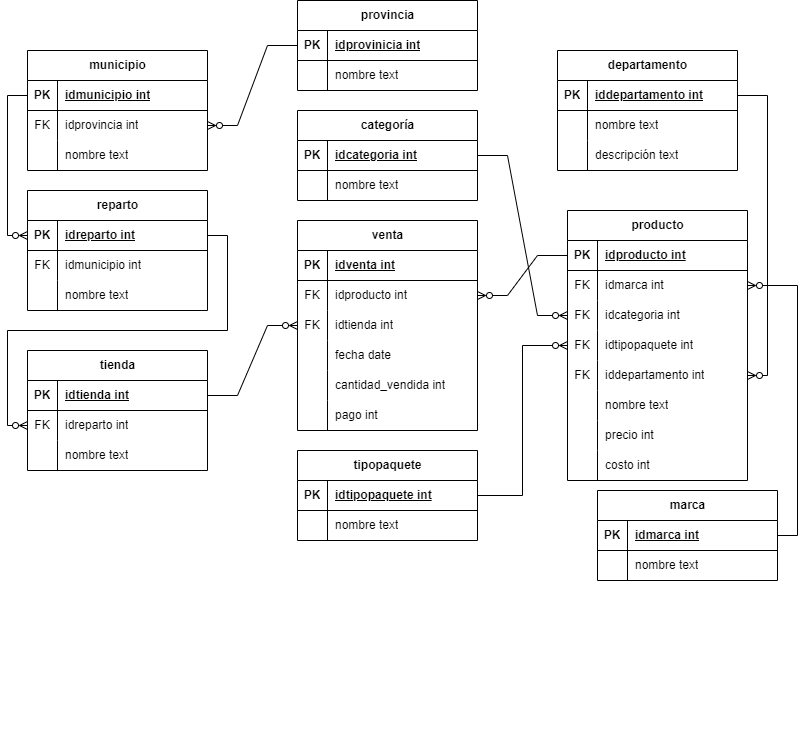
\includegraphics[scale=0.5]{Graphics/retailSales-Transactional.drawio.png}
    \caption{Sistema Transaccional: Ventas Minoristas}
    \label{fig:retail-transactional}
  \end{figure}

Los archivos que intervienen en este experimento se encuentran en la carpeta \textbf{retail\_sales} del 
directorio \textbf{experiments}. La definición del esquema estrella a poblar se encuentra en el archivo 
\textbf{retailsales.txt}, el listado de código \ref{retailsalesstar} muestra su contenido. La figura \ref{fig:retail-Warehouse} muestra la composición de las 
tablas de dimensión y de hechos del esquema estrella propuesto. 

\begin{lstlisting}[label={retailsalesstar}, caption={Definici\'on del esquema estrella del almacén de datos asociado al escenario ventas minoristas}]
  dimension tienda {
  tienda: idtienda PK
  tienda:nombre
  reparto:nombre as reparto
  municipio:nombre as municipio 1
  provincia:nombre as provincia 2
  }

  dimension producto {
  producto:idproducto PK
  marca:nombre as marca
  categoria:nombre as categoria
  tipopaquete:nombre as paquete
  departamento:nombre as departamento
  departamento:descripcion as descripcion
  producto:nombre as producto
  producto:precio
  producto:costo
  }

  dimension fecha {
  venta:fecha PK
  venta:week_day(fecha) str as Dia
  venta:month_str(fecha) str as Mes 1
  }

  fact venta {
  self:idventa PK serial
  venta:idproducto FK to producto.idproducto 
  venta:idtienda FK to tienda.idtienda
  venta:fecha FK to fecha.fecha
  venta:sum(cantidad_vendida) as cantidad_vendida_total
  venta:sum(pago) as importe_total
  producto:Costo * venta:sum(cantidad_vendida) int as coste_total
  venta:sum(pago) - producto:Costo * venta:sum(cantidad_vendida) int as ganancia 
  }
\end{lstlisting}

\begin{figure}
    \centering
    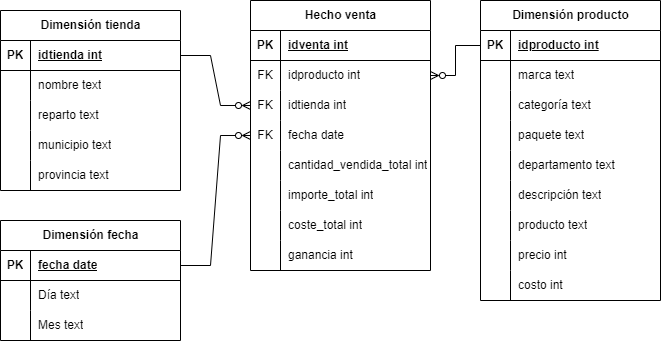
\includegraphics[scale=0.5]{Graphics/retailSales-Data Warehouse.drawio.png}
    \caption{Almacén de Datos: Ventas Minoristas}
    \label{fig:retail-Warehouse}
\end{figure}

\subsubsection{Fase 1: Exploraci\'on del Crawler y creaci\'on de la base de datos de Neo4j}

Para el esquema de base de datos de la figura \ref{fig:retail-transactional} la base de datos de Neo4j derivada a 
partir de los datos recopilados por el Crawler se muestra en la figura \ref{fig:catalogexp1}.

\begin{figure}
  \centering
  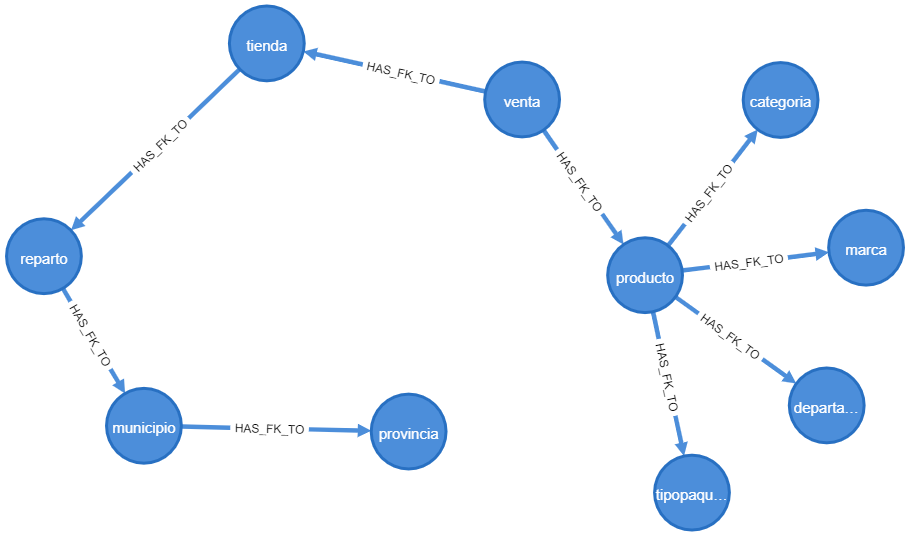
\includegraphics[scale=0.4]{Graphics/graph (1).png}
  \caption{Grafo de Neo4j para el esquema de ventas minoristas}
  \label{fig:catalogexp1}
\end{figure}

\subsubsection{Fase 2: Creaci\'on del grafo de join y \'arboles de join}

A partir de la base de datos de Neo4j obtenido en la fase 1 se computan el grafo de join y el \'arbol de 
join que se muestran en la figura \ref{fig:graphjoin1} y en la figura \ref{fig:jointree1} respectivamente. Para este caso, 
el \'arbol de join es \'unico y coincide  con el grafo de join debido a que el esquema de bases de datos de 
las ventas minoristas no presenta ambigüedades.

\begin{figure}
  \centering
  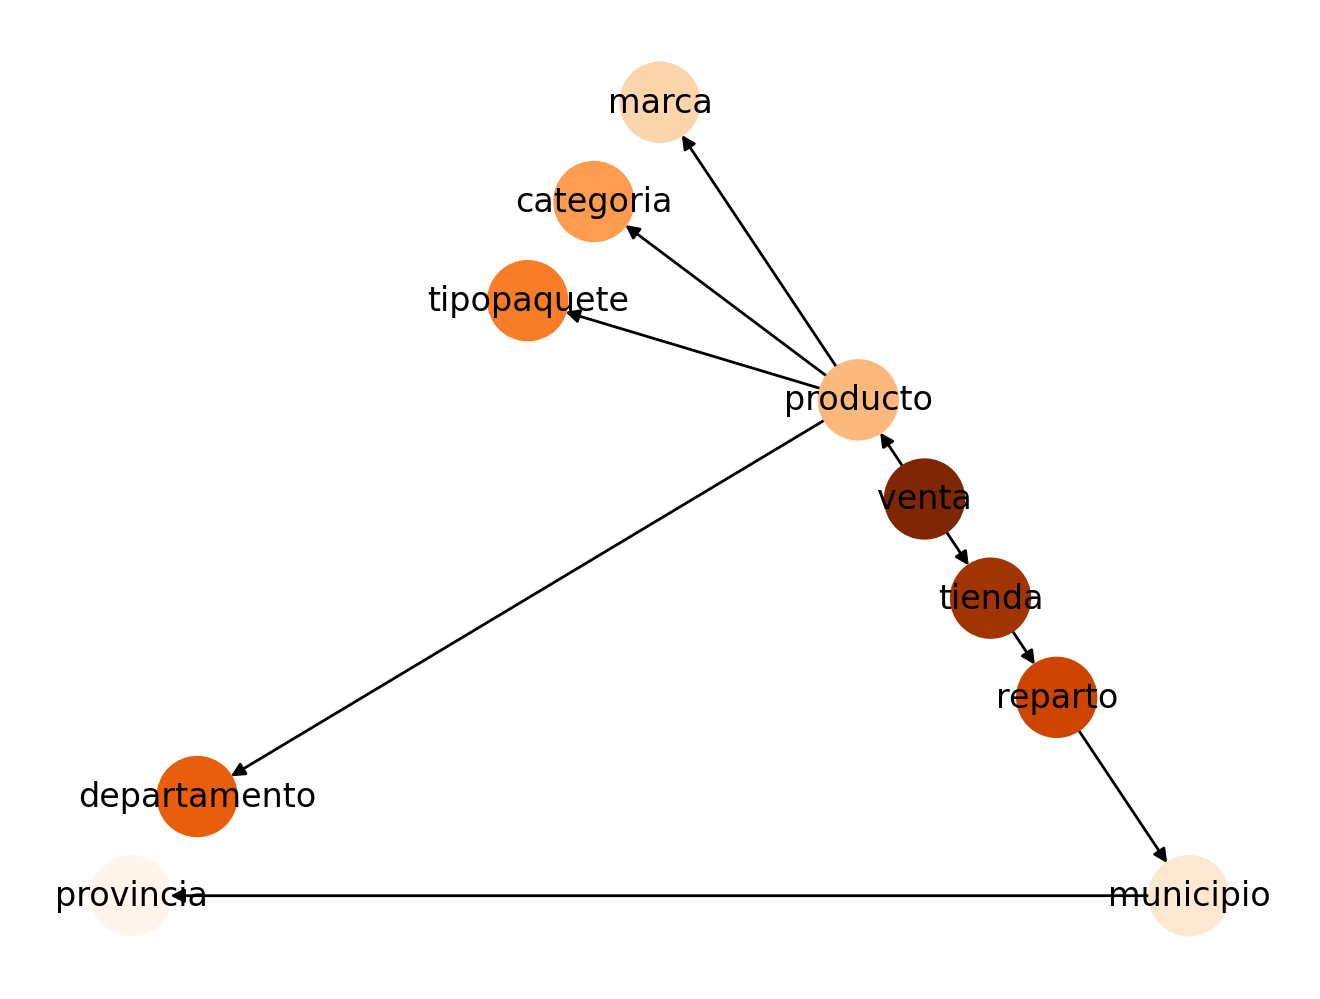
\includegraphics[scale=0.6]{Graphics/joingraph1.png}
  \caption{Grafo de join para el esquema de ventas minoristas}
  \label{fig:graphjoin1}
\end{figure}

\begin{figure}
  \centering
  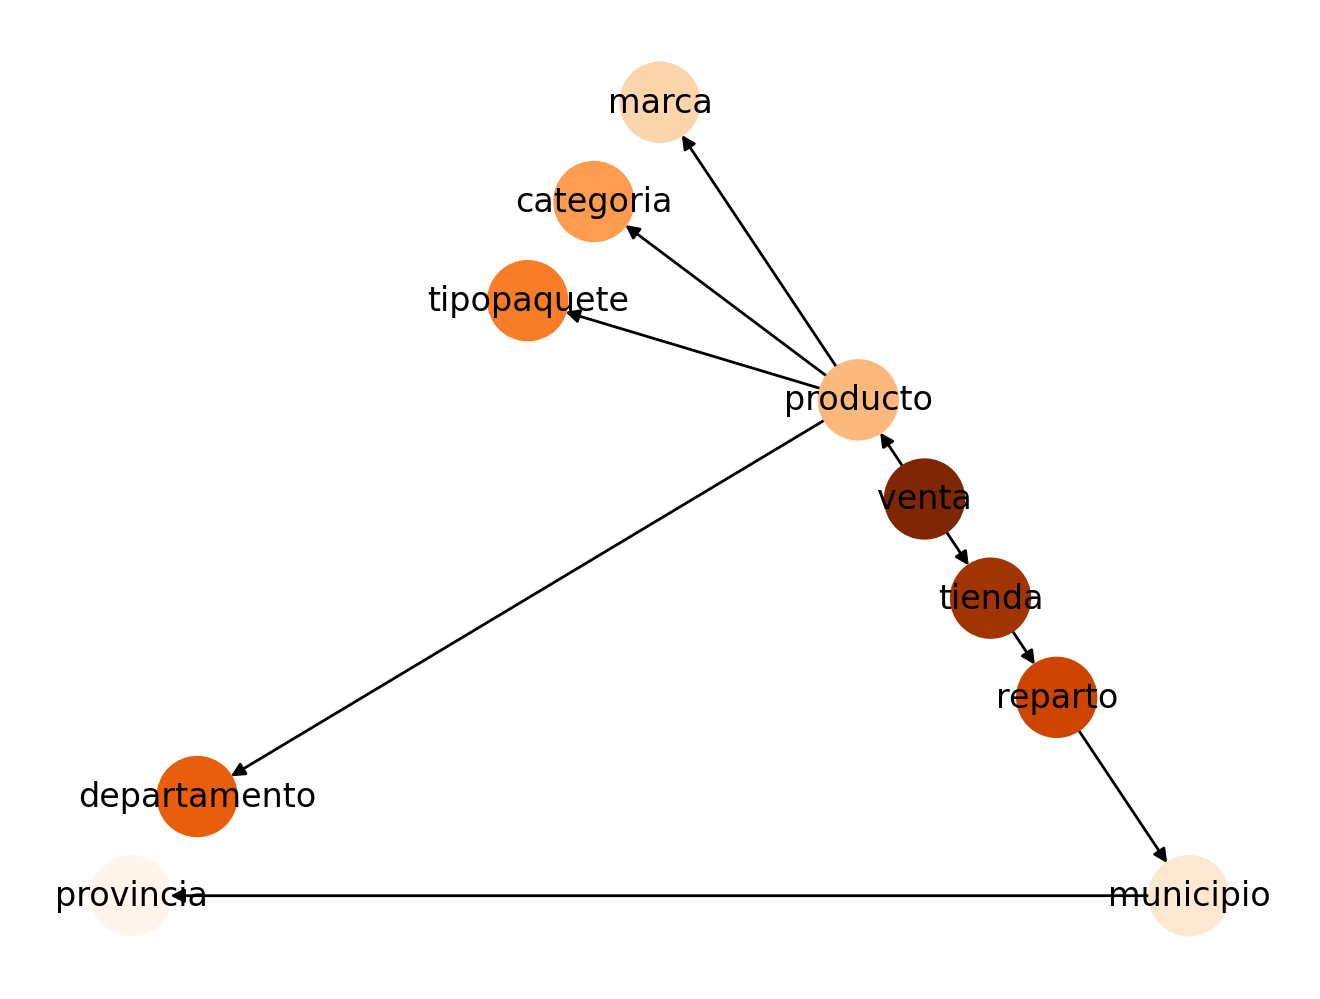
\includegraphics[scale=0.6]{Graphics/jointree1.png}
  \caption{\'Arbol de join para el esquema de ventas minoristas}
  \label{fig:jointree1}
\end{figure}

\subsubsection{Fase 3: Generaci\'on de las consultas}

La selección de los joins por parte del usuario se efectúa a través de la interfaz de usuario. 
Como solo hay un \'arbol de join hay una \'unica opción de join para 
cada tabla del esquema estrella. El listado de código \ref{joinselectexp1} muestra los joins 
computados a partir del \'arbol de join mostrado en la fase 2 y de la definición del esquema estrella 
presente en \textbf{retailsales.txt}.

\begin{lstlisting}[label={joinselectexp1}, caption={Joins computados para el experimento 1}, language={sql}]
  -- Joins for tienda
  1: tienda JOIN reparto ON tienda.idreparto = reparto.idreparto 
     JOIN municipio ON reparto.idmunicipio = municipio.idmunicipio 
     JOIN provincia ON municipio.idprovincia = provincia.idprovincia

  -- Joins for producto
  1: producto JOIN departamento ON producto.iddepartamento = departamento.iddepartamento 
     JOIN tipopaquete ON producto.idtipopaquete = tipopaquete.idtipopaquete 
     JOIN categoria ON producto.idcategoria = categoria.idcategoria 
     JOIN marca ON producto.idmarca = marca.idmarca

  -- Joins for fecha
  1: venta

  -- Joins for venta
  1: venta JOIN producto ON venta.idproducto = producto.idproducto
  
\end{lstlisting}

El listado de código \ref{quercreateexp1} muestra las consultas de creación y el listado de código 
\ref{selectexp1} muestra las consultas de selección, generadas a partir de los joins computados en 
la fase previa.

\begin{lstlisting}[label={quercreateexp1}, caption={Consultas de creaci\'on generadas para el experimento 1}, language={sql}]
  -- Creation query's
  CREATE TABLE IF NOT EXISTS fecha (
  fecha DATE, 
  Dia TEXT, 
  Mes TEXT, 
  PRIMARY KEY (fecha)
  );

  CREATE TABLE IF NOT EXISTS producto (
  idproducto INT, 
  marca TEXT, 
  categoria TEXT, 
  paquete TEXT, 
  departamento TEXT, 
  descripcion TEXT, 
  producto TEXT, 
  precio INT, 
  costo INT, 
  PRIMARY KEY (idproducto)
  );

  CREATE TABLE IF NOT EXISTS tienda (
  idtienda INT, 
  nombre TEXT, 
  reparto TEXT, 
  municipio TEXT, 
  provincia TEXT, 
  PRIMARY KEY (idtienda)
  );

  CREATE TABLE IF NOT EXISTS venta (
  idventa serial, 
  idproducto INT, 
  idtienda INT, 
  fecha DATE, 
  cantidad_vendida_total INT, 
  importe_total INT, 
  coste_total INT, 
  ganancia INT, 
  PRIMARY KEY (idventa), 
  FOREIGN KEY (idproducto) REFERENCES producto (idproducto), 
  FOREIGN KEY (idtienda) REFERENCES tienda (idtienda), 
  FOREIGN KEY (fecha) REFERENCES fecha (fecha), 
  UNIQUE(idproducto, idtienda, fecha)
  );

  -- level metadata
  CREATE TABLE IF NOT EXISTS level_metadata (
                                  table_name TEXT,
                                  attribute_name TEXT,
                                  level INT,
                                  PRIMARY KEY (table_name, attribute_name, level));

  INSERT INTO level_metadata VALUES('tienda', 'idtienda', 0);
  INSERT INTO level_metadata VALUES('tienda', 'nombre', 0);
  INSERT INTO level_metadata VALUES('tienda', 'reparto', 0);
  INSERT INTO level_metadata VALUES('tienda', 'municipio', 1);
  INSERT INTO level_metadata VALUES('tienda', 'provincia', 2);
  INSERT INTO level_metadata VALUES('producto', 'idproducto', 0);
  INSERT INTO level_metadata VALUES('producto', 'marca', 0);
  INSERT INTO level_metadata VALUES('producto', 'categoria', 0);
  INSERT INTO level_metadata VALUES('producto', 'paquete', 0);
  INSERT INTO level_metadata VALUES('producto', 'departamento', 0);
  INSERT INTO level_metadata VALUES('producto', 'descripcion', 0);
  INSERT INTO level_metadata VALUES('producto', 'producto', 0);
  INSERT INTO level_metadata VALUES('producto', 'precio', 0);
  INSERT INTO level_metadata VALUES('producto', 'costo', 0);
  INSERT INTO level_metadata VALUES('fecha', 'fecha', 0);
  INSERT INTO level_metadata VALUES('fecha', 'Dia', 0);
  INSERT INTO level_metadata VALUES('fecha', 'Mes', 1);
  INSERT INTO level_metadata VALUES('venta', 'idventa', 0);
  INSERT INTO level_metadata VALUES('venta', 'idproducto', 0);
  INSERT INTO level_metadata VALUES('venta', 'idtienda', 0);
  INSERT INTO level_metadata VALUES('venta', 'fecha', 0);
  INSERT INTO level_metadata VALUES('venta', 'cantidad_vendida_total', 0);
  INSERT INTO level_metadata VALUES('venta', 'importe_total', 0);
  INSERT INTO level_metadata VALUES('venta', 'coste_total', 0);
  INSERT INTO level_metadata VALUES('venta', 'ganancia', 0);
\end{lstlisting}

\begin{lstlisting}[label={selectexp1}, caption={Consultas de selecci\'on generadas para el experimento 1}, language={sql}]
  -- Selection for fecha
  SELECT DISTINCT venta.fecha, to_char(venta.fecha, 'Day') AS Dia, to_char(venta.fecha, 'Month') AS Mes
  FROM venta;

  -- Selection for producto
  SELECT DISTINCT producto.idproducto, marca.nombre AS marca, categoria.nombre AS categoria, tipopaquete.nombre AS paquete, departamento.nombre AS departamento, departamento.descripcion AS descripcion, producto.nombre AS producto, producto.precio, producto.costo
  FROM producto
  JOIN departamento ON producto.iddepartamento = departamento.iddepartamento
  JOIN tipopaquete ON producto.idtipopaquete = tipopaquete.idtipopaquete
  JOIN categoria ON producto.idcategoria = categoria.idcategoria
  JOIN marca ON producto.idmarca = marca.idmarca;

  -- Selection for tienda
  SELECT DISTINCT tienda.idtienda, tienda.nombre, reparto.nombre AS reparto, municipio.nombre AS municipio, provincia.nombre AS provincia
  FROM tienda
  JOIN reparto ON tienda.idreparto = reparto.idreparto
  JOIN municipio ON reparto.idmunicipio = municipio.idmunicipio
  JOIN provincia ON municipio.idprovincia = provincia.idprovincia;

  -- Selection for venta
  SELECT DISTINCT venta.idproducto, venta.idtienda, venta.fecha, SUM(venta.cantidad_vendida) AS cantidad_vendida_total, SUM(venta.pago) AS importe_total, producto.Costo*SUM(venta.cantidad_vendida) AS coste_total, SUM(venta.pago)-producto.Costo*SUM(venta.cantidad_vendida) AS ganancia
  FROM venta
  JOIN producto ON venta.idproducto = producto.idproducto
  GROUP BY venta.idproducto,venta.idtienda,venta.fecha,producto.Costo;
\end{lstlisting}

\subsubsection{Fase 4: Creaci\'on manual del pipeline y poblaci\'on del almac\'en de datos}

El pipeline creado se encuentra en la ruta \textbf{experiments/retail\_sales} con el nombre de 
\textbf{pipeline.py}. Este script utiliza las consultas generadas ejecutando su código utilizando 
Psycopg2.

La figura \ref{fig:fullpg1} muestra el estado del servidor de bases de datos \textbf{target} luego de la ejecución 
del pipeline. La figura muestra como efectivamente 
se han creado y poblado todas la tablas del esquema estrella definido.

\begin{figure}
  \centering
  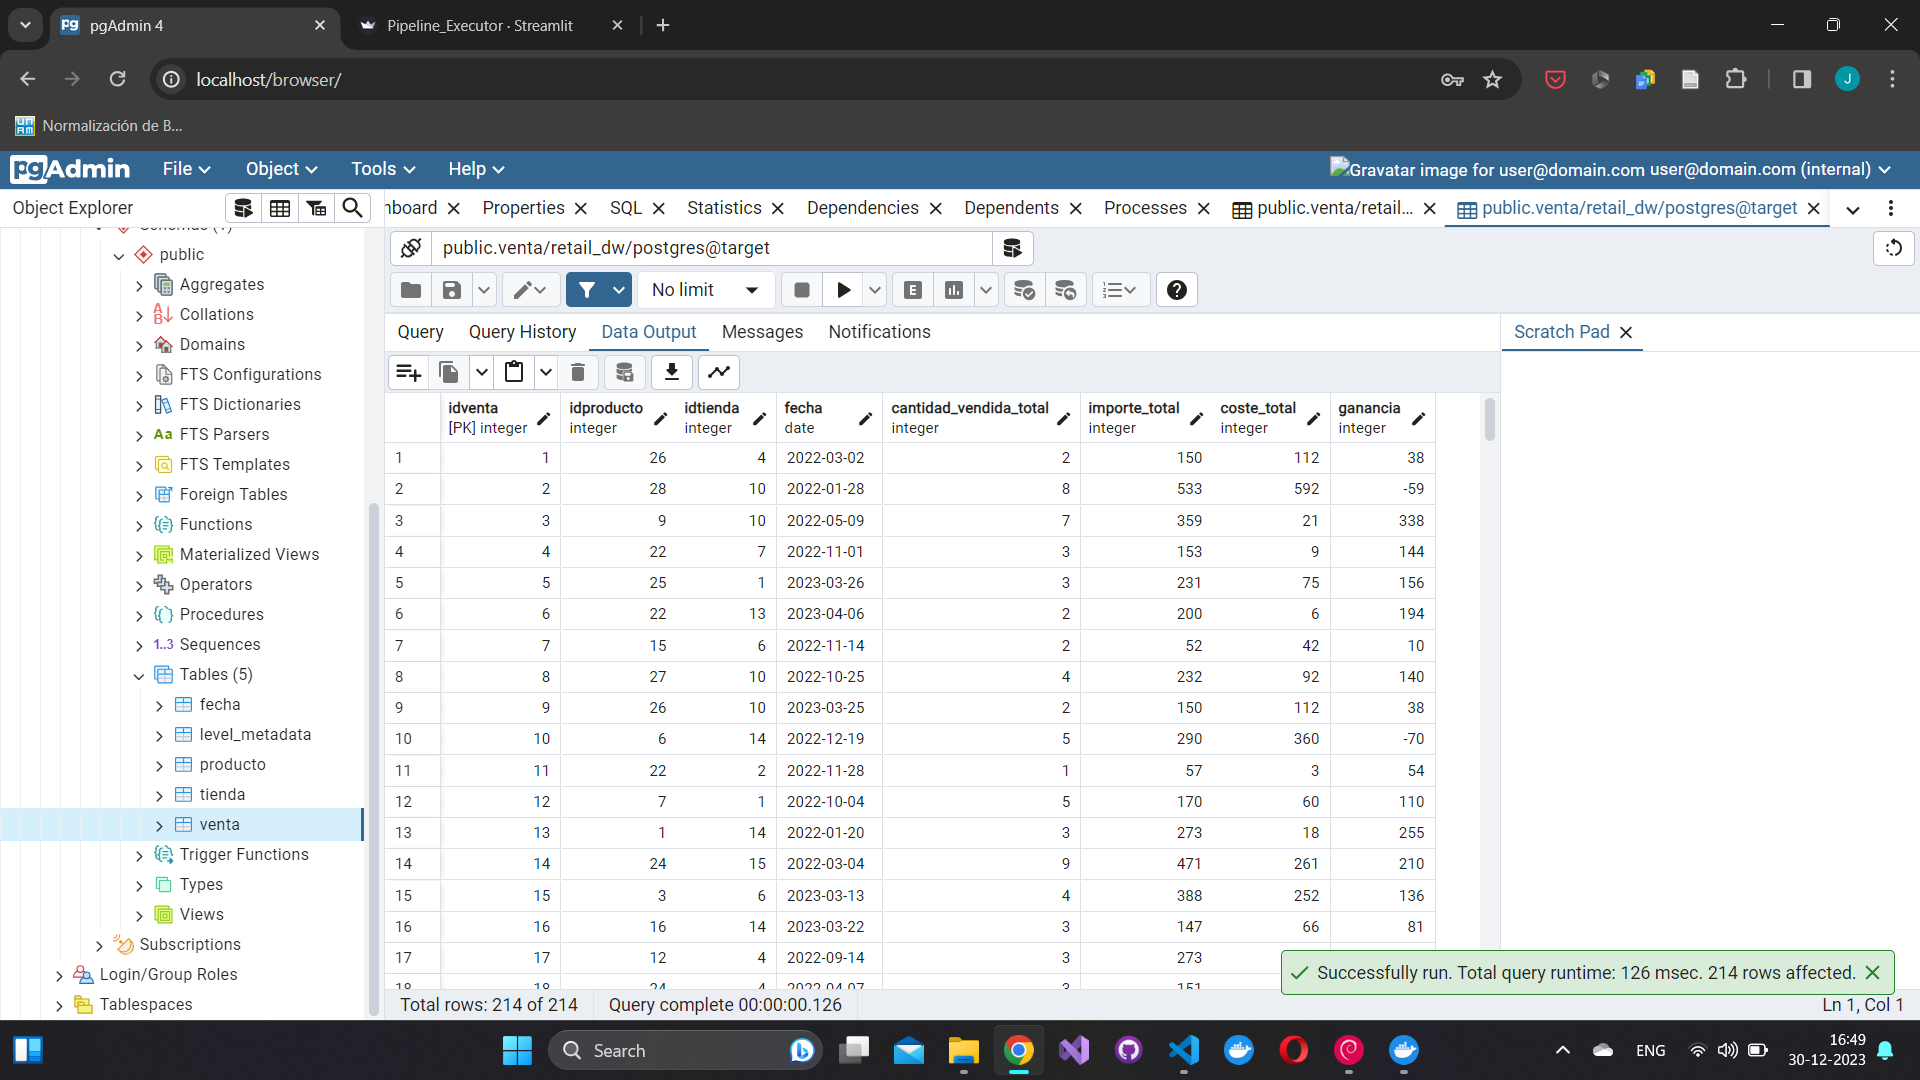
\includegraphics[scale=0.4]{Graphics/fullpgadmin1.png}
  \caption{Almacén de datos poblado asociado al escenario de ventas minoristas}
  \label{fig:fullpg1}
\end{figure}


\subsection{Experimento 2: Escenario TPCH}

Este escenario est\'a inspirado en el escenario de prueba TPCH\footnote{https://www.tpc.org/tpch/}, ampliamente 
utilizada para probar soluciones de bases de datos e Inteligencia de Negocios. Los scripts que participan 
en el proceso de creación y población de la base de datos de prueba TPCH se encuentran en la ruta 
\textbf{experiments/tpch}. La especificación del esquema estrella del almacén de datos a poblar se encuentra 
en el script del DSL \textbf{tpch.txt}, el listado de código \ref{tpchstar} muestra su contenido.  A continuación se describe el escenario que modela la base de datos.

\begin{lstlisting}[label={tpchstar}, caption={Definici\'on del esquema estrella del almacén de datos asociado al escenario TPCH}]
  dimension supplier {
    supplier: s_suppkey PK as suppkey
    supplier: s_name as name
    supplier: s_phone as phone
    supplier: s_address as address
    nation: n_name as nation
    region: r_name as region 1
  }

  dimension part {
      part: p_partkey PK
      part: p_name as name
      part: p_brand as brand
      part: p_size
      part: p_retailprice
  }

  dimension order_date {
      orders: o_orderdate PK as o_date
      orders:week_day(o_orderdate) str as day
      orders:month_str(o_orderdate) str as month 1
  }

  fact lineitem {
      self: linenumber PK serial as lnumber
      lineitem: l_partkey FK to part.p_partkey as partkey
      lineitem: l_suppkey FK to supplier.suppkey as supplierkey
      orders: o_orderdate FK to order_date.o_date as order_date
      lineitem: sum(l_payment) as totalpayment
      lineitem: sum(l_quantity) as totalquantity
      lineitem: sum(l_payment) - (lineitem: sum(l_quantity) * partsupp:ps_supplycost) - (lineitem: sum(l_quantity) * part:p_retailprice) numeric as earnings
  }
\end{lstlisting}

Una distribuidora vende piezas de varios suministradores. Distintos suministradores pueden 
producir la misma pieza. Los clientes de la suministradora realizan \'ordenes de compra 
de piezas de determinados suministradores. La figura  muestra el esquema de bases de datos 
del escenario TPCH. La figura \ref{fig:transactionaltpch} muestra el esquema de base de datos 
del escenario descrito.

\begin{figure}
  \centering
  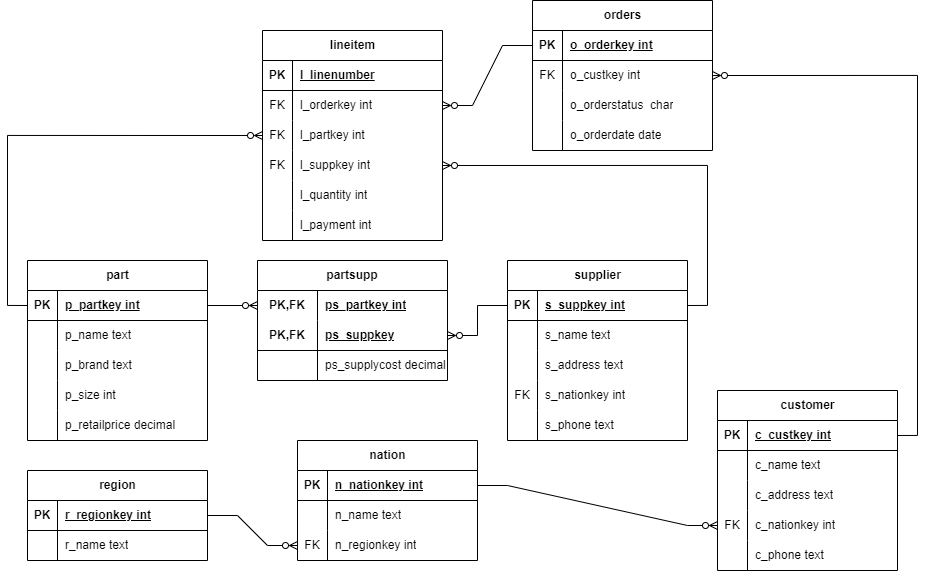
\includegraphics[scale=0.5]{Graphics/tpch-tpch-transactional.drawio (4).png}
  \caption{Esquema de la base de datos TPCH}
  \label{fig:transactionaltpch}
\end{figure}

La figura \ref{fig:warehousetpch} muestra el almacén de datos \textbf{tpch\_dw} que se poblar\'a a partir de los 
datos de la base de datos \textbf{TPCH}.

\begin{figure}
  \centering
  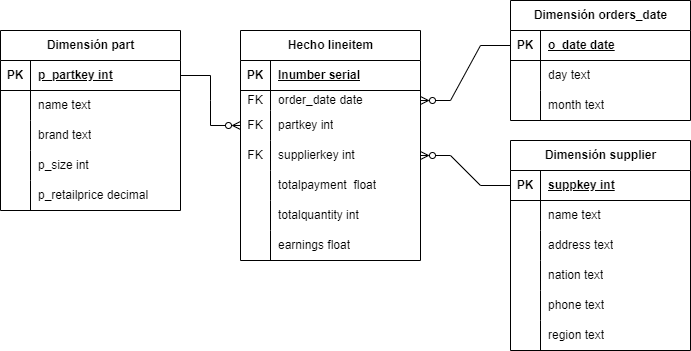
\includegraphics[scale=0.5]{Graphics/tpch-tpch-warehouse.drawio.png}
  \caption{Almacén de datos tpch\_dw}
  \label{fig:warehousetpch}
\end{figure}

\subsubsection{Fase 1: Exploraci\'on del Crawler y creaci\'on de la base de datos de Neo4j}

Para el esquema de base de datos de la figura \ref{fig:transactionaltpch} la base de datos de Neo4j derivada a 
partir de los datos recopilados por el Crawler se muestra en la figura \ref{fig:catalogexp2}.

\begin{figure}
  \centering
  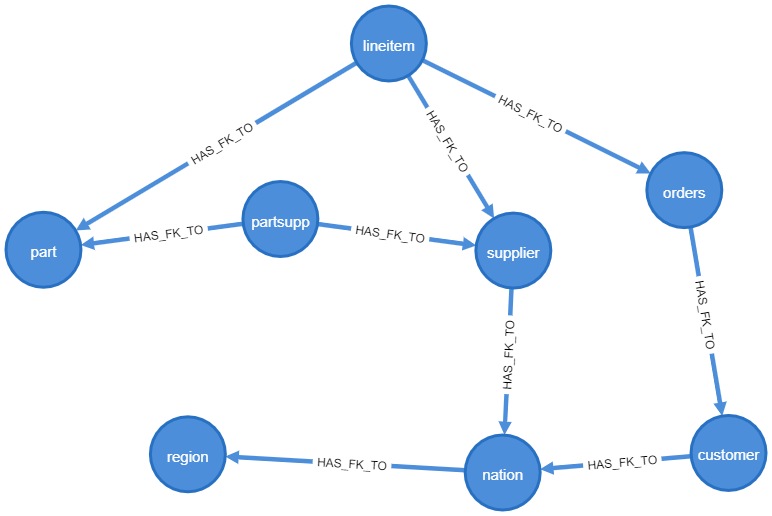
\includegraphics[scale=0.4]{Graphics/graph (2).png}
  \caption{Grafo de Neo4j para el esquema de TPCH}
  \label{fig:catalogexp2}
\end{figure}

\subsubsection{Fase 2: Creaci\'on del grafo de join y \'arboles de join}

A partir de la base de datos de Neo4j obtenido en la fase 1 se computan el grafo de join y los \'arboles de 
join que se muestran en la figura \ref{fig:graphjoin2} y en la figura \ref{fig:jointree2} respectivamente. 
N\'otese como en TPCH no existe una relaci\'on directa entre las tablas \textbf{Lineitem} y \textbf{PartSupplier}, 
sin embargo en el grafo de join se incluye un arco entre ellos dado que cumplen con el criterio expuesto 
en el cap\'itulo \ref{chapter:proposal} para la formaci\'on de arcos entre dos nodos del grafo de join.

\begin{figure}
  \centering
  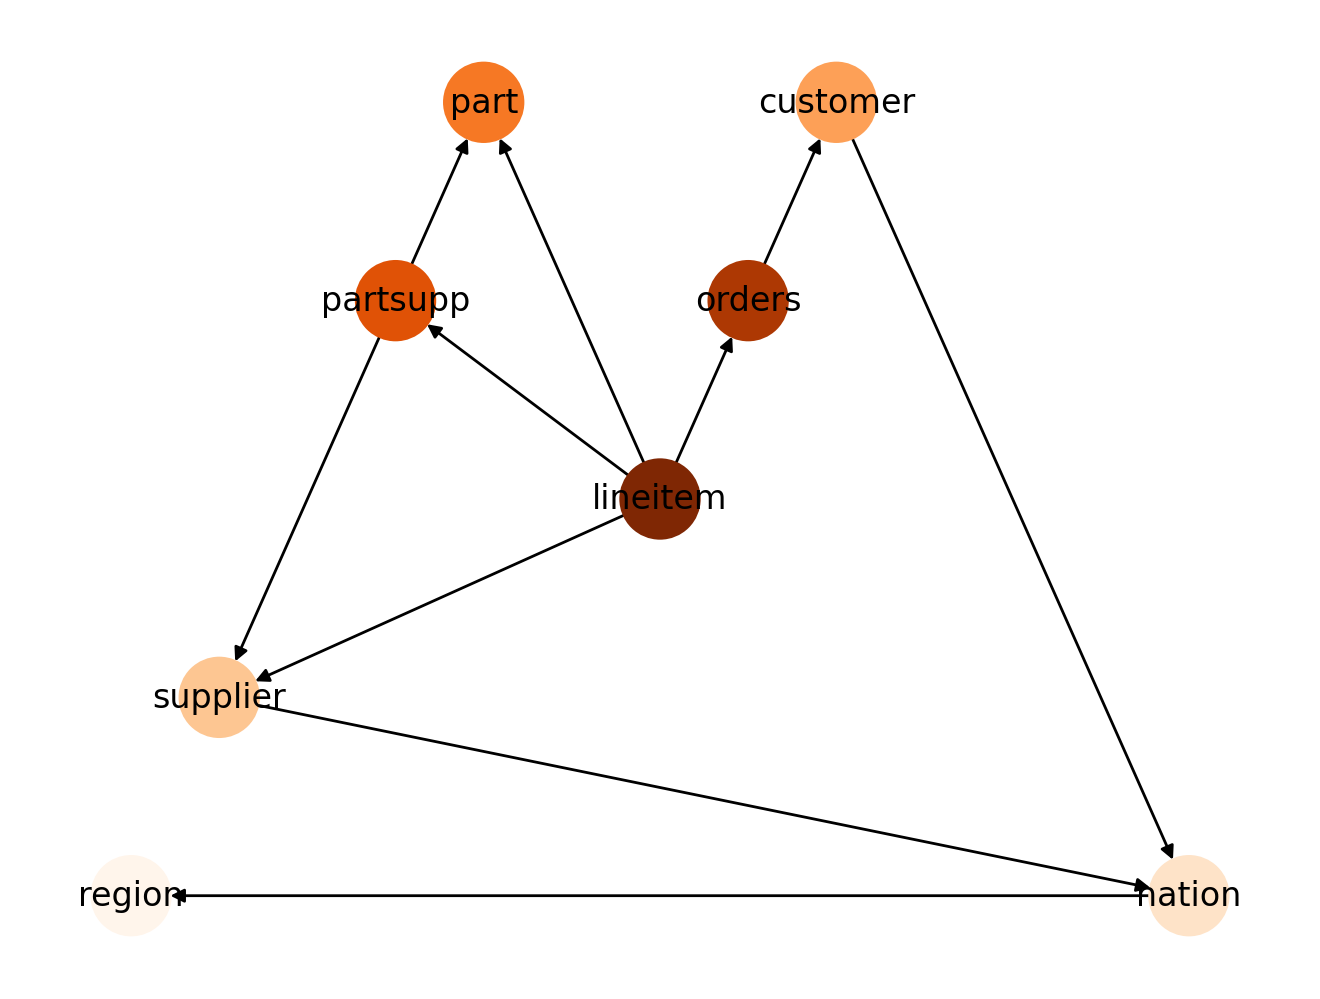
\includegraphics[scale=0.6]{Graphics/joingraph2.png}
  \caption{Grafo de join para el esquema de TPCH}
  \label{fig:graphjoin2}
\end{figure}

\begin{figure}
  \centering
  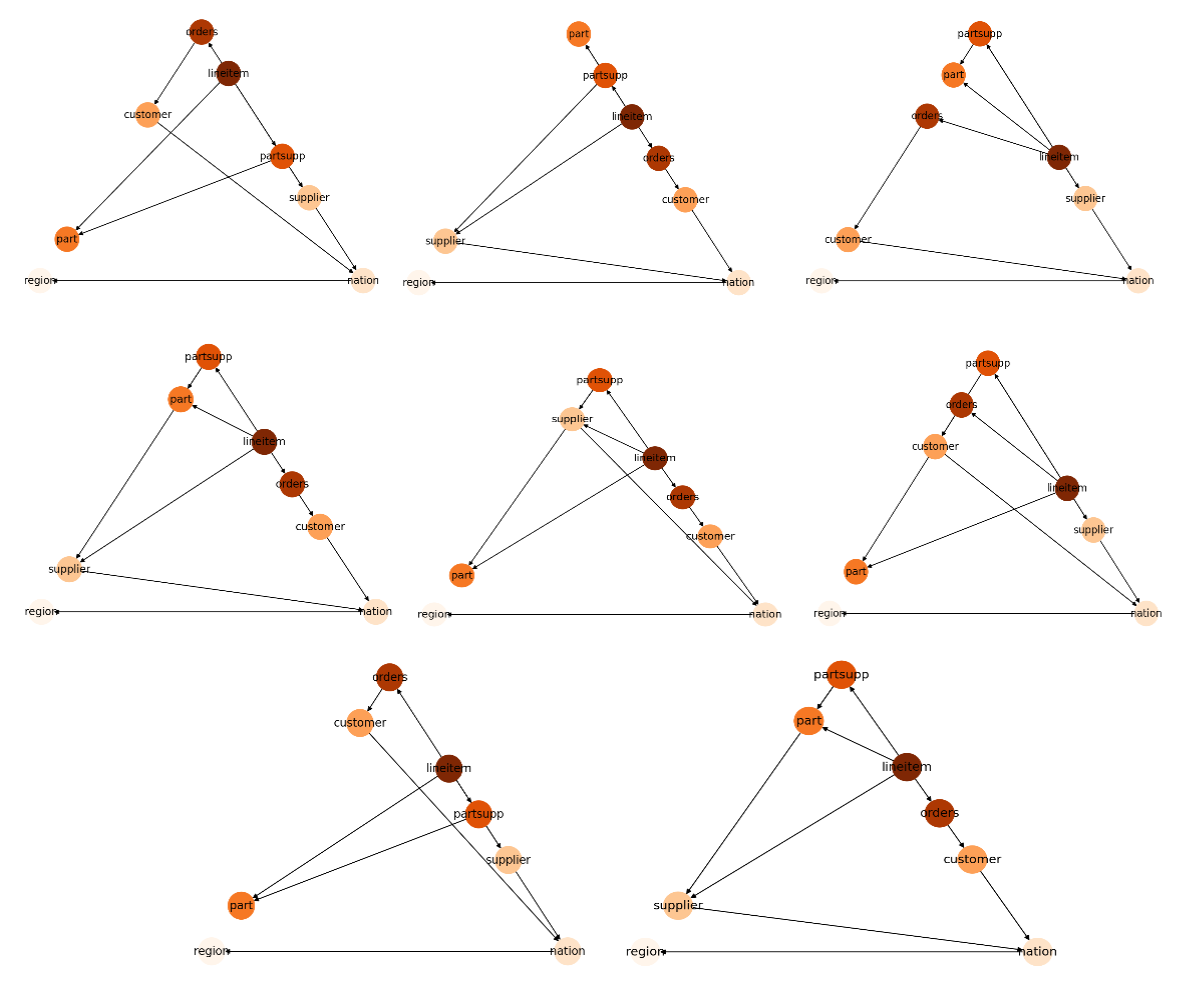
\includegraphics[scale=0.4]{Graphics/jointreesexp2.png}
  \caption{\'Arboles de join para el esquema de TPCH}
  \label{fig:jointree2}
\end{figure}

\subsubsection{Fase 3: Generaci\'on de las consultas}

Los joins computados para la poblaci\'on de cada una de las tablas del esquema estrella del almacén de datos 
\textbf{tpch\_dw} presente en el script del DSL \textbf{tpch.tex} son los siguientes: 

\begin{lstlisting}[label={joinsexp2}, caption={Joins computados para el experimento 2}, language={sql}]
  -- Joins for supplier
  1: supplier JOIN nation ON supplier.s_nationkey = nation.n_nationkey 
     JOIN region ON nation.n_regionkey = region.r_regionkey

  2: lineitem JOIN orders ON lineitem.l_orderkey = orders.o_orderkey 
    JOIN customer ON orders.o_custkey = customer.c_custkey 
    JOIN nation ON customer.c_nationkey = nation.n_nationkey 
    JOIN region ON nation.n_regionkey = region.r_regionkey 
    JOIN partsupp ON lineitem.l_suppkey = partsupp.ps_suppkey AND lineitem.l_partkey = partsupp.ps_partkey 
    JOIN supplier ON partsupp.ps_suppkey = supplier.s_suppkey

  3: lineitem JOIN supplier ON lineitem.l_suppkey = supplier.s_suppkey 
    JOIN orders ON lineitem.l_orderkey = orders.o_orderkey 
    JOIN customer ON orders.o_custkey = customer.c_custkey 
    JOIN nation ON customer.c_nationkey = nation.n_nationkey 
    JOIN region ON nation.n_regionkey = region.r_regionkey

  -- Joins for part
  1: part

  -- Joins for order_date
  1: orders

  -- Joins for lineitem
  1: lineitem JOIN orders ON lineitem.l_orderkey = orders.o_orderkey 
     JOIN partsupp ON lineitem.l_suppkey = partsupp.ps_suppkey AND lineitem.l_partkey = partsupp.ps_partkey 
     JOIN part ON partsupp.ps_partkey = part.p_partkey

  2: lineitem JOIN part ON lineitem.l_partkey = part.p_partkey 
     JOIN orders ON lineitem.l_orderkey = orders.o_orderkey 
     JOIN partsupp ON lineitem.l_suppkey = partsupp.ps_suppkey AND lineitem.l_partkey = partsupp.ps_partkey
\end{lstlisting}

Para el caso de \textbf{part} y \textbf{orders} no es necesario un join por tanto todos los datos se obtienen de 
una sola tabla. 

Seleccionando en todos los casos el primer join mostrado en el listado de c\'odigo \ref{joinsexp2} se generan 
las consultas de creaci\'on mostradas en el listado c\'odigo \ref{genquery2} y las consultas de selecci\'on 
mostradas en el listado de c\'odigo \ref{selectexp2}: 

\begin{lstlisting}[label={genquery2}, caption={Consultas de creaci\'on generadas para el experimento 2}, language={sql}]
  -- Creation query's
  CREATE TABLE IF NOT EXISTS lineitem (
  lnumber serial, 
  partkey INT, 
  supplierkey INT, 
  order_date DATE, 
  totalpayment FLOAT, 
  totalquantity INT, 
  earnings NUMERIC, 
  PRIMARY KEY (lnumber), 
  FOREIGN KEY (partkey) REFERENCES part (p_partkey), 
  FOREIGN KEY (supplierkey) REFERENCES supplier (suppkey), 
  FOREIGN KEY (order_date) REFERENCES order_date (o_date), 
  UNIQUE(partkey, supplierkey, order_date)
  );

  CREATE TABLE IF NOT EXISTS order_date (
  o_date DATE, 
  day TEXT, 
  month TEXT, 
  PRIMARY KEY (o_date)
  );

  CREATE TABLE IF NOT EXISTS part (
  p_partkey INT, 
  name TEXT, 
  brand TEXT, 
  p_size INT, 
  p_retailprice NUMERIC, 
  PRIMARY KEY (p_partkey)
  );

  CREATE TABLE IF NOT EXISTS supplier (
  suppkey INT, 
  name TEXT, 
  phone TEXT, 
  address TEXT, 
  nation TEXT, 
  region TEXT, 
  PRIMARY KEY (suppkey)
  );

  -- level metadata 
  CREATE TABLE IF NOT EXISTS level_metadata (
                                  table_name TEXT,
                                  attribute_name TEXT,
                                  level INT,
                                  PRIMARY KEY (table_name, attribute_name, level));

  INSERT INTO level_metadata VALUES('supplier', 'suppkey', 0);
  INSERT INTO level_metadata VALUES('supplier', 'name', 0);
  INSERT INTO level_metadata VALUES('supplier', 'phone', 0);
  INSERT INTO level_metadata VALUES('supplier', 'address', 0);
  INSERT INTO level_metadata VALUES('supplier', 'nation', 0);
  INSERT INTO level_metadata VALUES('supplier', 'region', 1);
  INSERT INTO level_metadata VALUES('part', 'p_partkey', 0);
  INSERT INTO level_metadata VALUES('part', 'name', 0);
  INSERT INTO level_metadata VALUES('part', 'brand', 0);
  INSERT INTO level_metadata VALUES('part', 'p_size', 0);
  INSERT INTO level_metadata VALUES('part', 'p_retailprice', 0);
  INSERT INTO level_metadata VALUES('order_date', 'o_date', 0);
  INSERT INTO level_metadata VALUES('order_date', 'day', 0);
  INSERT INTO level_metadata VALUES('order_date', 'month', 1);
  INSERT INTO level_metadata VALUES('lineitem', 'lnumber', 0);
  INSERT INTO level_metadata VALUES('lineitem', 'partkey', 0);
  INSERT INTO level_metadata VALUES('lineitem', 'supplierkey', 0);
  INSERT INTO level_metadata VALUES('lineitem', 'order_date', 0);
  INSERT INTO level_metadata VALUES('lineitem', 'totalpayment', 0);
  INSERT INTO level_metadata VALUES('lineitem', 'totalquantity', 0);
  INSERT INTO level_metadata VALUES('lineitem', 'earnings', 0);
\end{lstlisting}

\begin{lstlisting}[label={selectexp2}, caption={Consultas de selecci\'on generadas para el experimento 2}, language={sql}]
  -- Selection for lineitem
  SELECT DISTINCT lineitem.l_partkey AS partkey, lineitem.l_suppkey AS supplierkey, orders.o_orderdate AS order_date, SUM(lineitem.l_payment) AS totalpayment, SUM(lineitem.l_quantity) AS totalquantity, SUM(lineitem.l_payment)-(SUM(lineitem.l_quantity)*partsupp.ps_supplycost)-(SUM(lineitem.l_quantity)*part.p_retailprice) AS earnings
  FROM lineitem
  JOIN orders ON lineitem.l_orderkey = orders.o_orderkey
  JOIN partsupp ON lineitem.l_suppkey = partsupp.ps_suppkey AND lineitem.l_partkey = partsupp.ps_partkey
  JOIN part ON partsupp.ps_partkey = part.p_partkey
  GROUP BY lineitem.l_partkey,lineitem.l_suppkey,orders.o_orderdate,partsupp.ps_supplycost,part.p_retailprice;

  -- Selection for order_date
  SELECT DISTINCT orders.o_orderdate AS o_date, to_char(orders.o_orderdate, 'Day') AS day, to_char(orders.o_orderdate, 'Month') AS month
  FROM orders;

  -- Selection for part 
  SELECT DISTINCT part.p_partkey, part.p_name AS name, part.p_brand AS brand, part.p_size, part.p_retailprice
  FROM part;

  -- Selection for supplier 
  SELECT DISTINCT supplier.s_suppkey AS suppkey, supplier.s_name AS name, supplier.s_phone AS phone, supplier.s_address AS address, nation.n_name AS nation, region.r_name AS region
  FROM supplier
  JOIN nation ON supplier.s_nationkey = nation.n_nationkey
  JOIN region ON nation.n_regionkey = region.r_regionkey;
\end{lstlisting}

\subsubsection{Fase 4: Creaci\'on manual del pipeline y poblaci\'on del almac\'en de datos}

El pipeline creado se encuentra en la ruta \textbf{experiments/tpch} con el nombre de 
\textbf{pipeline.py}. 

La figura \ref{fig:fullpg2} muestra el estado del servidor de bases de datos \textbf{target} luego de la ejecuci\'on 
del pipeline, y nuevamente se puede constatar la correcta poblaci\'on del almac\'en de datos \textbf{tpch\_dw}.

\begin{figure}
  \centering
  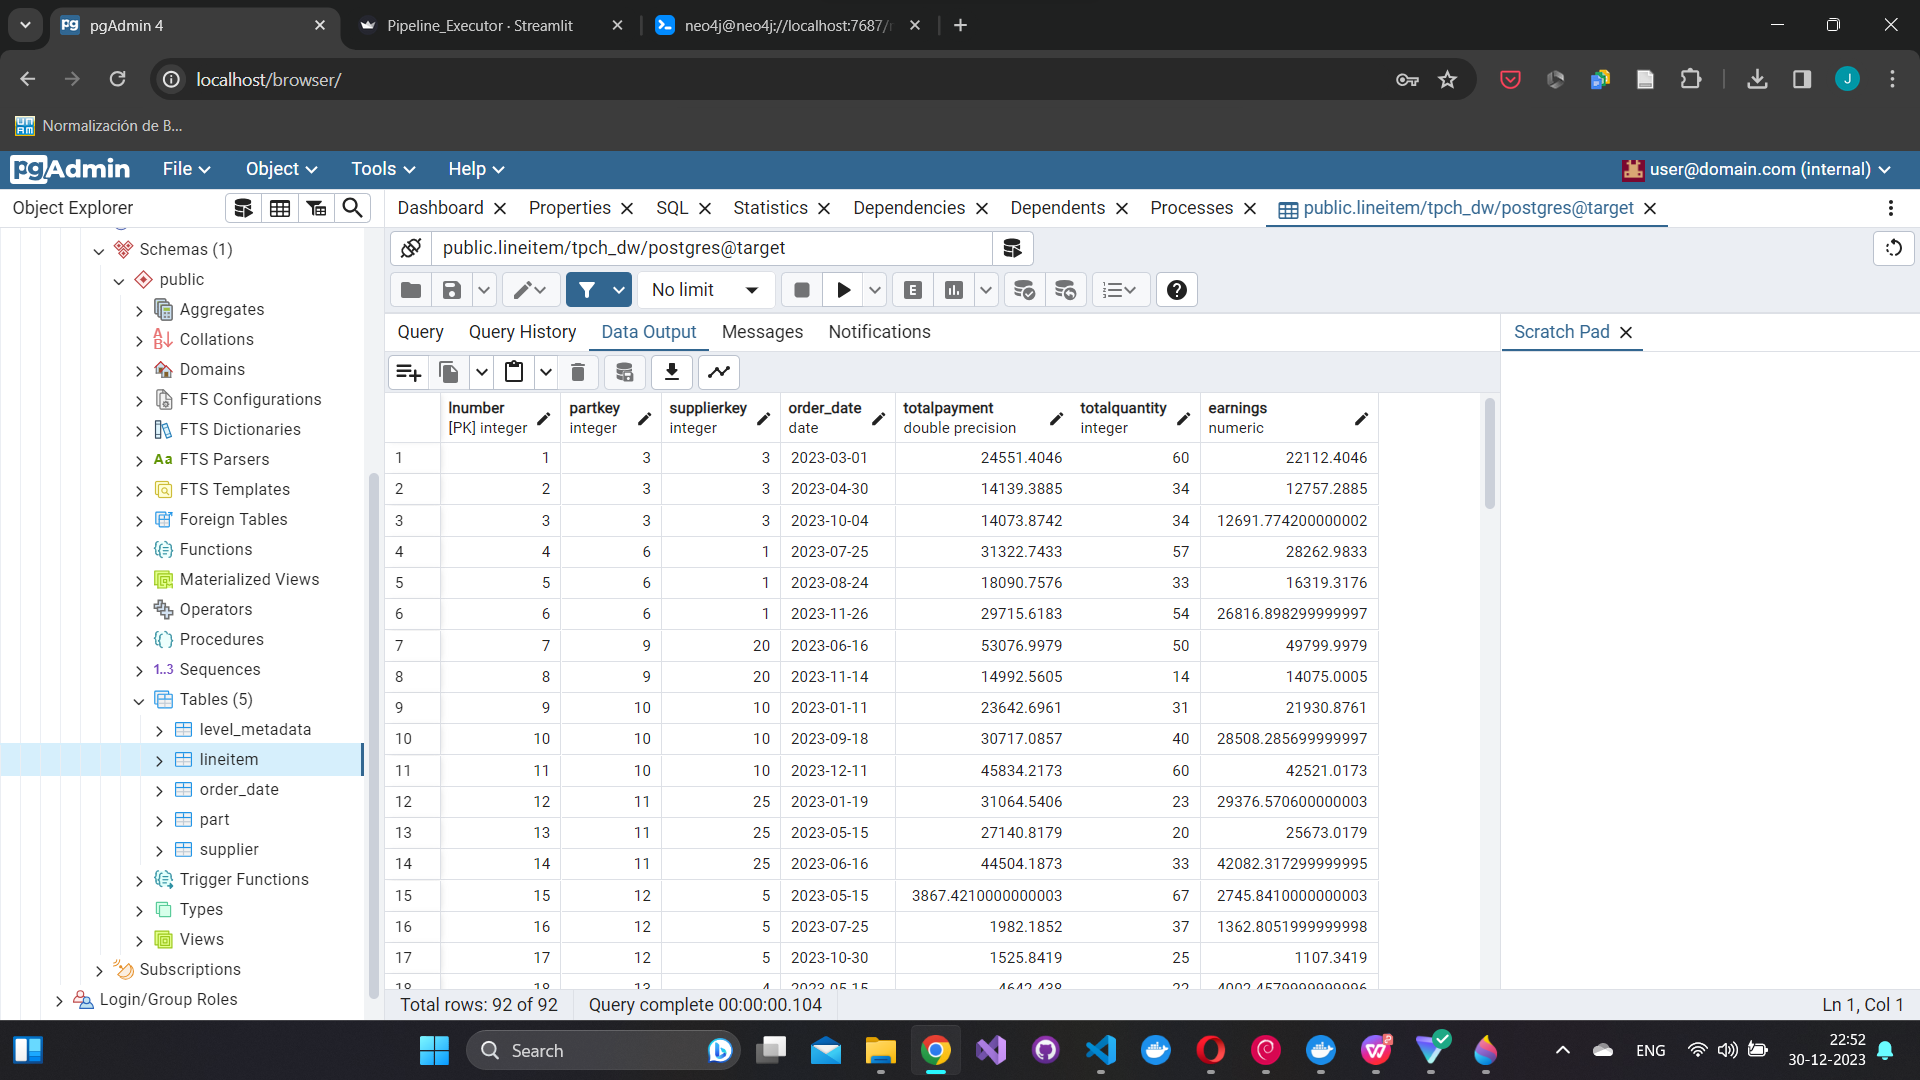
\includegraphics[scale=0.4]{Graphics/fullpgadmin2.png}
  \caption{Almacén de datos poblado asociado al escenario de TPCH}
  \label{fig:fullpg2}
\end{figure}




\backmatter

\begin{conclusions}
    El objetivo fundamental de este trabajo fue realizar una primera aproximaci\'on a la generaci\'on 
    autom\'atica de procesos ETL mediante el enfrentamiento del problema de la inferencia de joins. 

    A partir del estudio del estado de arte sobre la inferencia de joins y la automatizaci\'on de procesos 
    ETL se diseña un lenguaje de dominio espec\'ifico para la definici\'on de escenarios anal\'iticos que 
    vincula el modelo relacional y el modelo dimensional, el cual constituye el principal aporte de la 
    presente investigaci\'on. Adem\'as, se desarrolló un prototipo funcional de un marco de trabajo extensible 
    e independiente de los sistemas de gestión de bases de datos. Este marco, partiendo de la definición de un 
    escenario analítico mediante el lenguaje de dominio específico concebido, es capaz de generar consultas para la 
    extracción 
    de datos y la creación de tablas, infiriendo adecuadamente una conjunto joins necesarios para estas consultas, 
    con el 
    objetivo de poblar automáticamente el escenario definido. Sin embargo, debido a limitaciones de tiempo, no se 
    logró concretar una implementación para la generación de pipelines que utilicen las consultas generadas, las 
    ejecuten en un orden lógico e inserten los datos extra\'idos en el sistema destino
    para lograr la población efectiva de los escenarios analíticos definidos.

    Se ejecutaron experimentos que permitieron establecer la validez de la propuesta realizada y evidenciaron el 
    correcto funcionamiento del prototipo implementado.
\end{conclusions}

\begin{recomendations}
A partir de los desafíos computacionales encontrados, así como de los resultados
obtenidos por el sistema desarrollado, se identifican nuevas líneas de investigación que
permitan mejorar la efectividad del marco de trabajo propuesto:

\begin{itemize}
    \item Implementaci\'on de un generador de pipelines, gen\'erico e independientes de los sistemas 
        de gestión de bases de datos, para la poblaci\'on automática de los escenarios analíticos definidos en los 
        que adem\'as se les pueda configurar el tipo de extracción de datos y de carga a utilizar.
        
    \item El prototipo implementado necesita la intervención del usuario para seleccionar los joins
        de las consultas de selecci\'on. Se propone la implementaci\'on de un sistema que permita 
        analizar la semántica de los joins computados y seleccione de forma autom\'atica el join 
        m\'as conveniente para la consulta que se ha de generar.

    \item Enriquecimiento del lenguaje de dominio espec\'ifico concebido para abarcar otros aspectos 
        de la definición de modelos dimensionales tales como la granularidad y la aditividad. 
        
    \item Enriquecimiento del lenguaje de dominio espec\'ifico y del marco de trabajo diseñado 
        para lograr la automatizaci\'on de otros procesos de la integraci\'on de datos, además de la inferencia 
        de joins.
\end{itemize}

\end{recomendations}

\begin{annexes}
    \begin{figure}
        \centering
        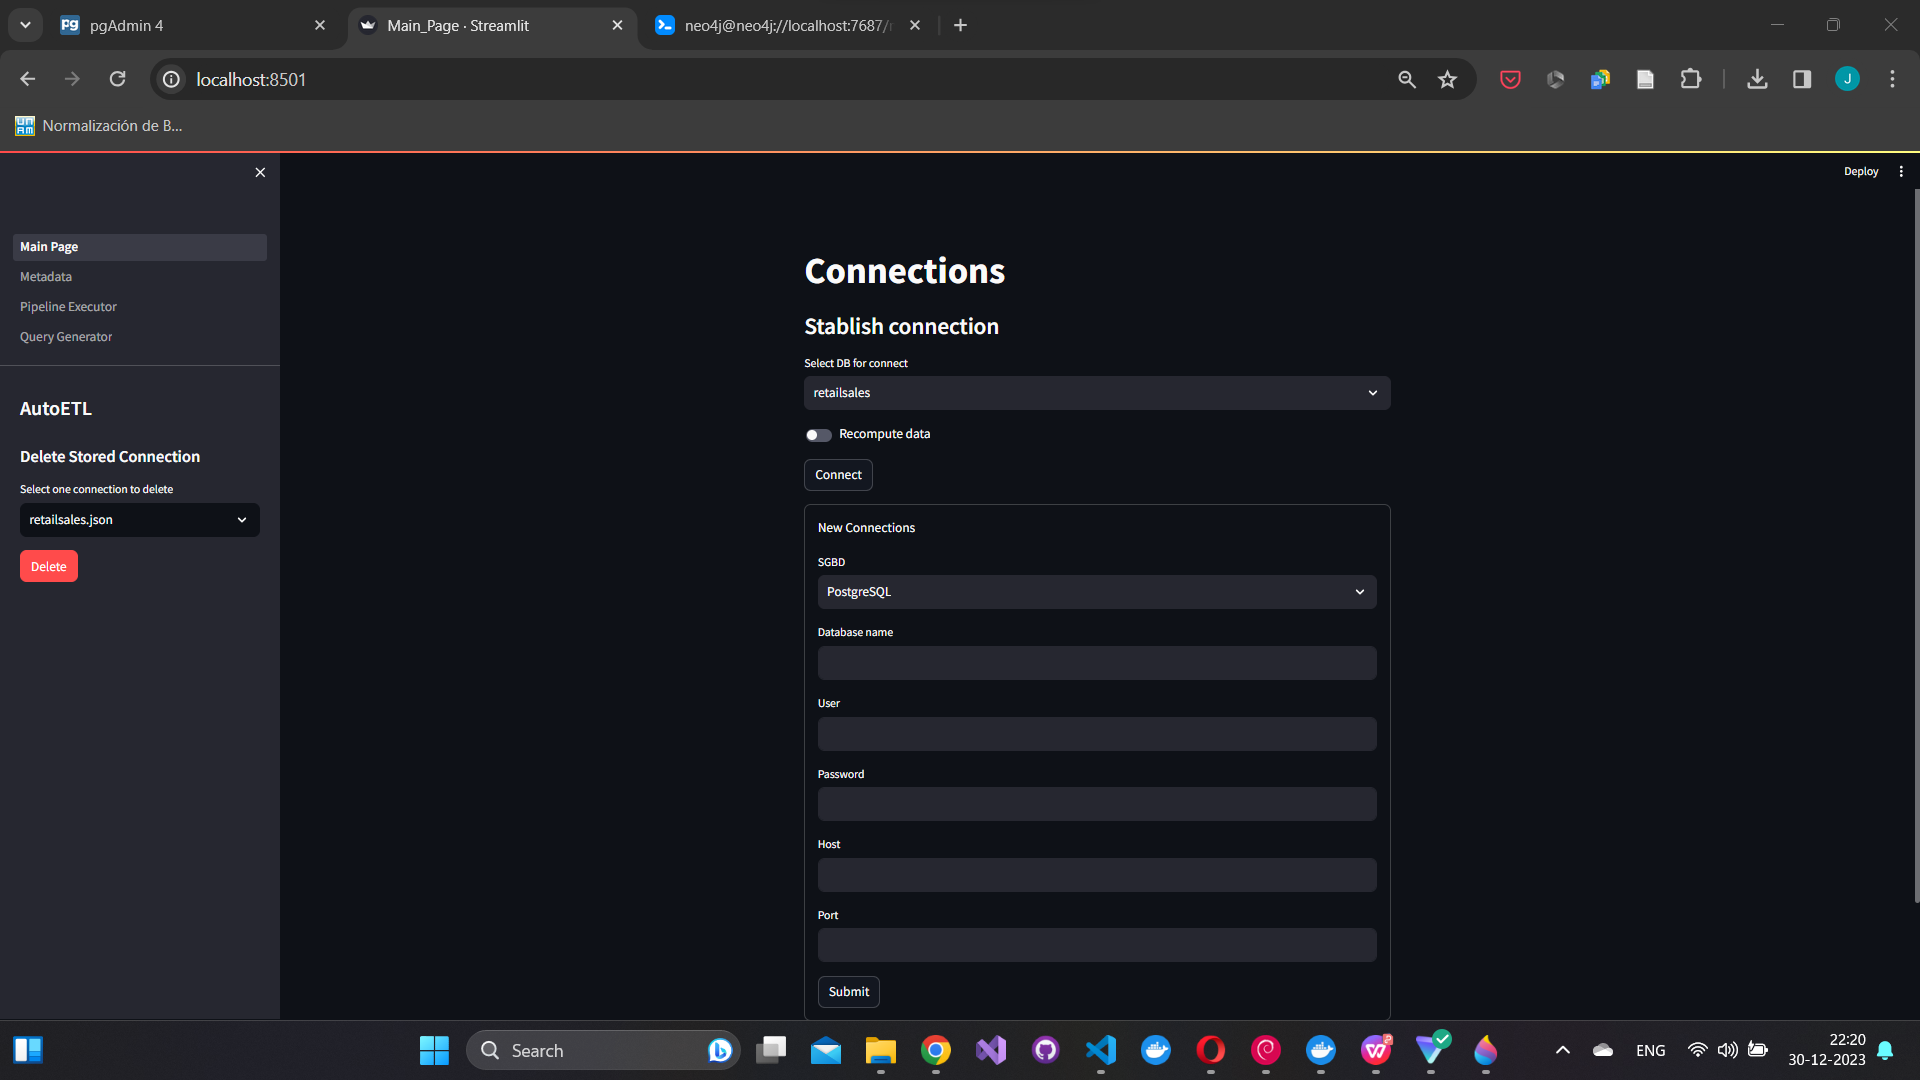
\includegraphics[scale=0.4]{Graphics/mainpage.png}
        \caption{Im\'agen de la p\'agina Main Page.}
        \label{fig:mainpage}
      \end{figure}

    \begin{figure}
        \centering
        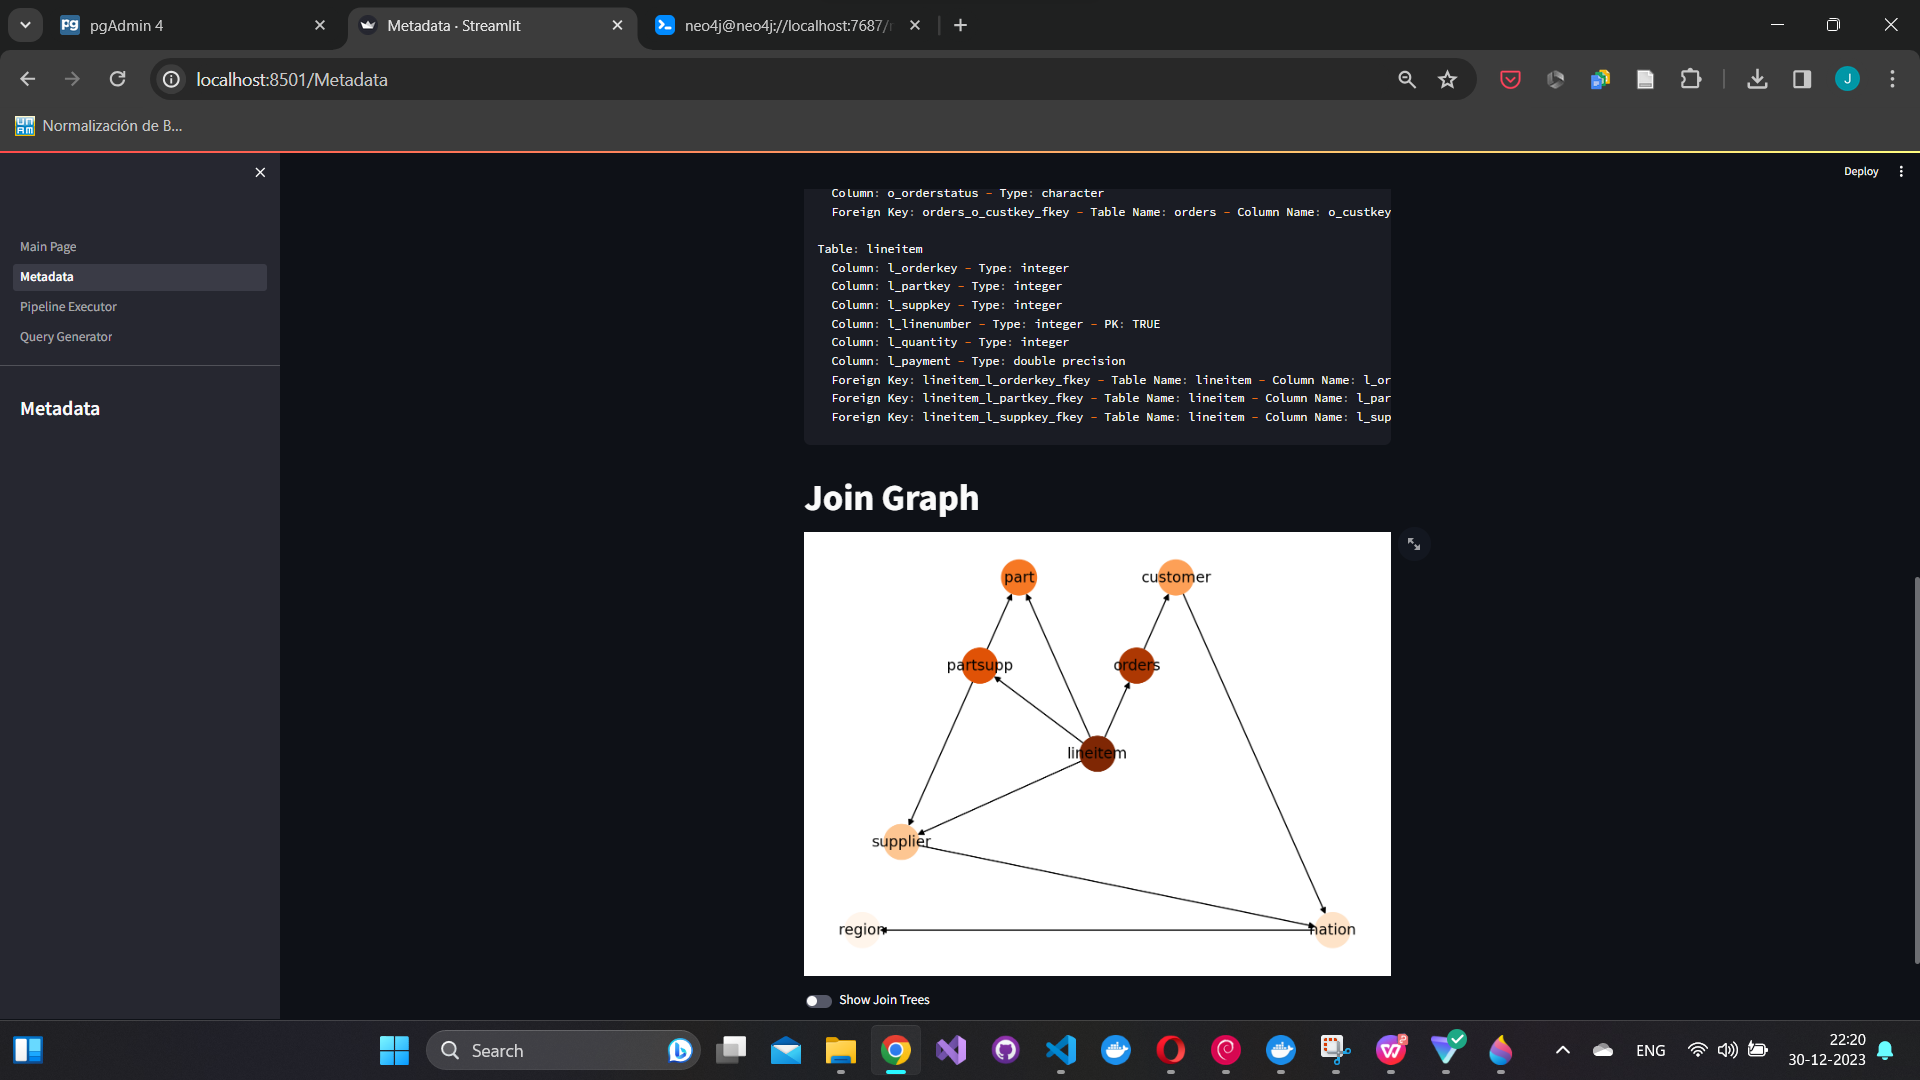
\includegraphics[scale=0.4]{Graphics/metadata.png}
        \caption{Im\'agen de la p\'agina Metadata.}
        \label{fig:meta}
    \end{figure}

    \begin{figure}
        \centering
        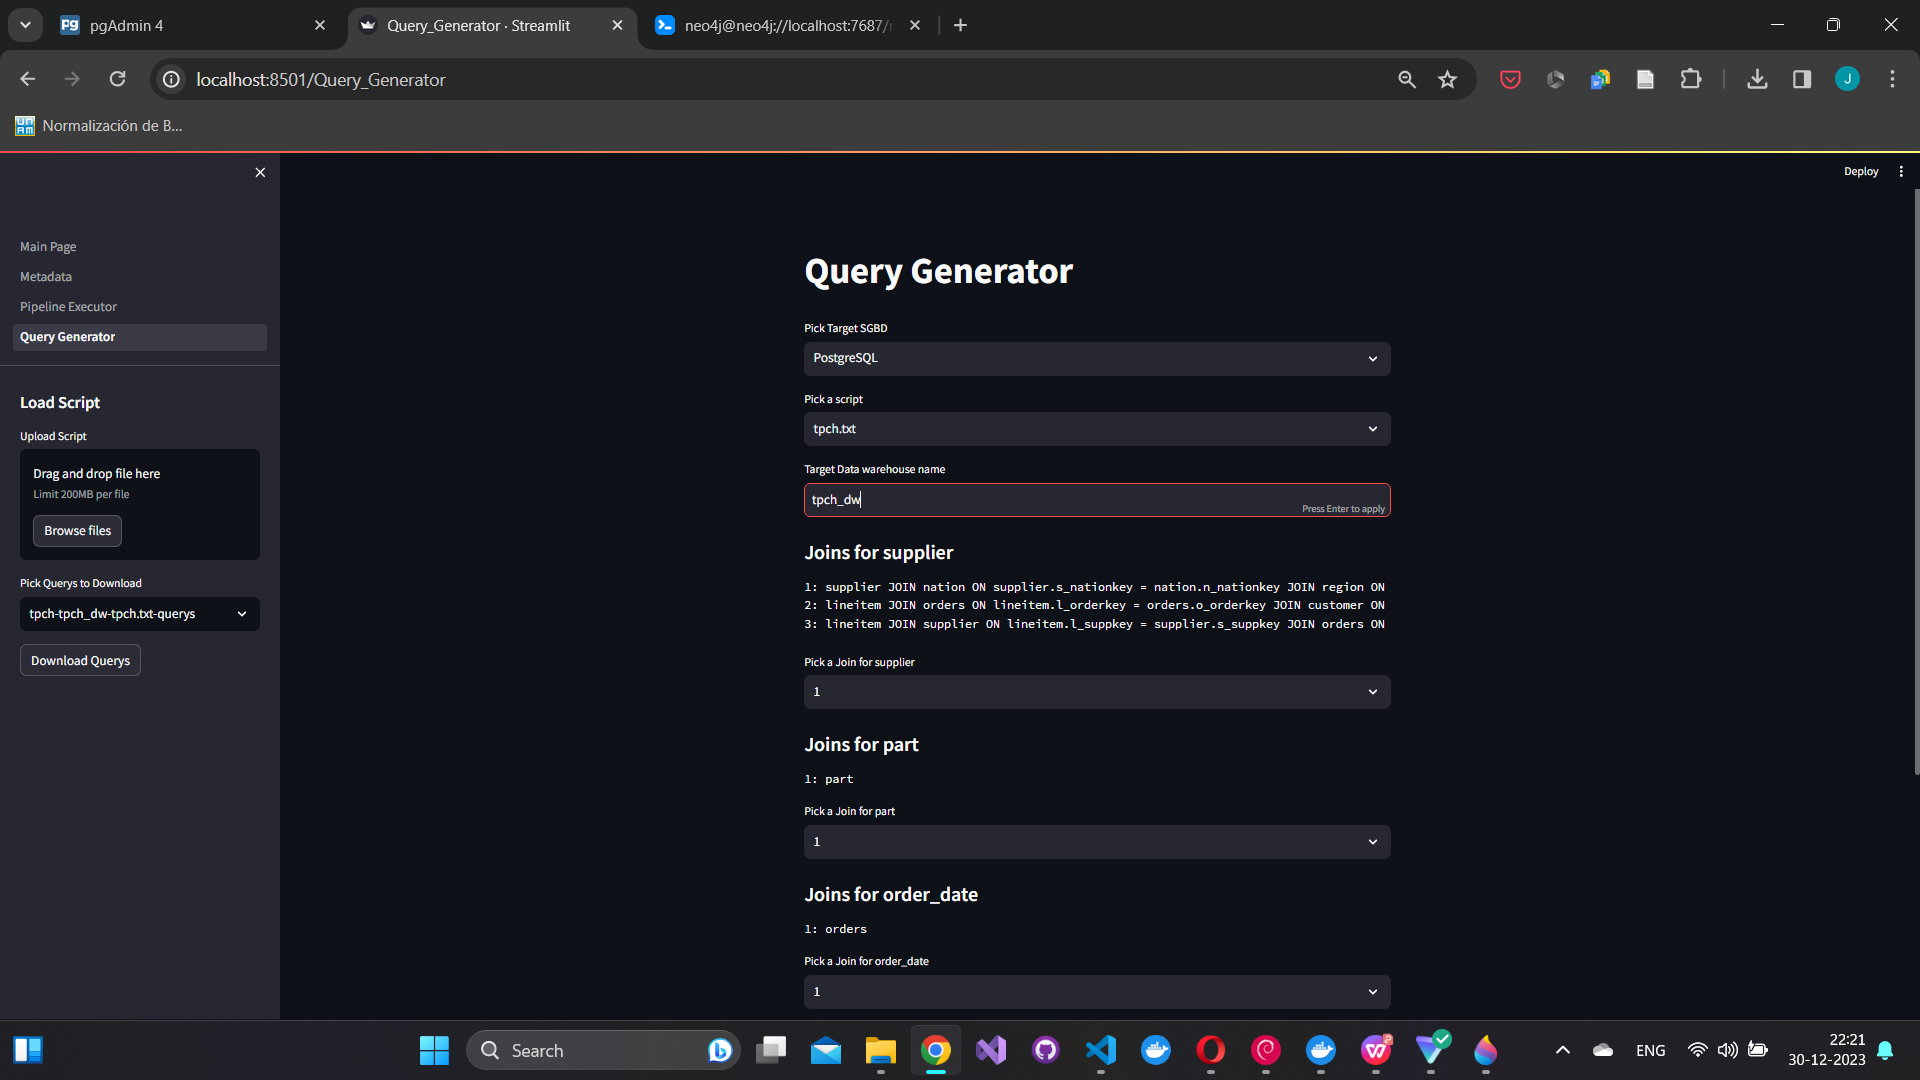
\includegraphics[scale=0.4]{Graphics/querygene.png}
        \caption{Im\'agen de la p\'agina Query Generator.}
        \label{fig:generator}
    \end{figure}

    \begin{figure}
        \centering
        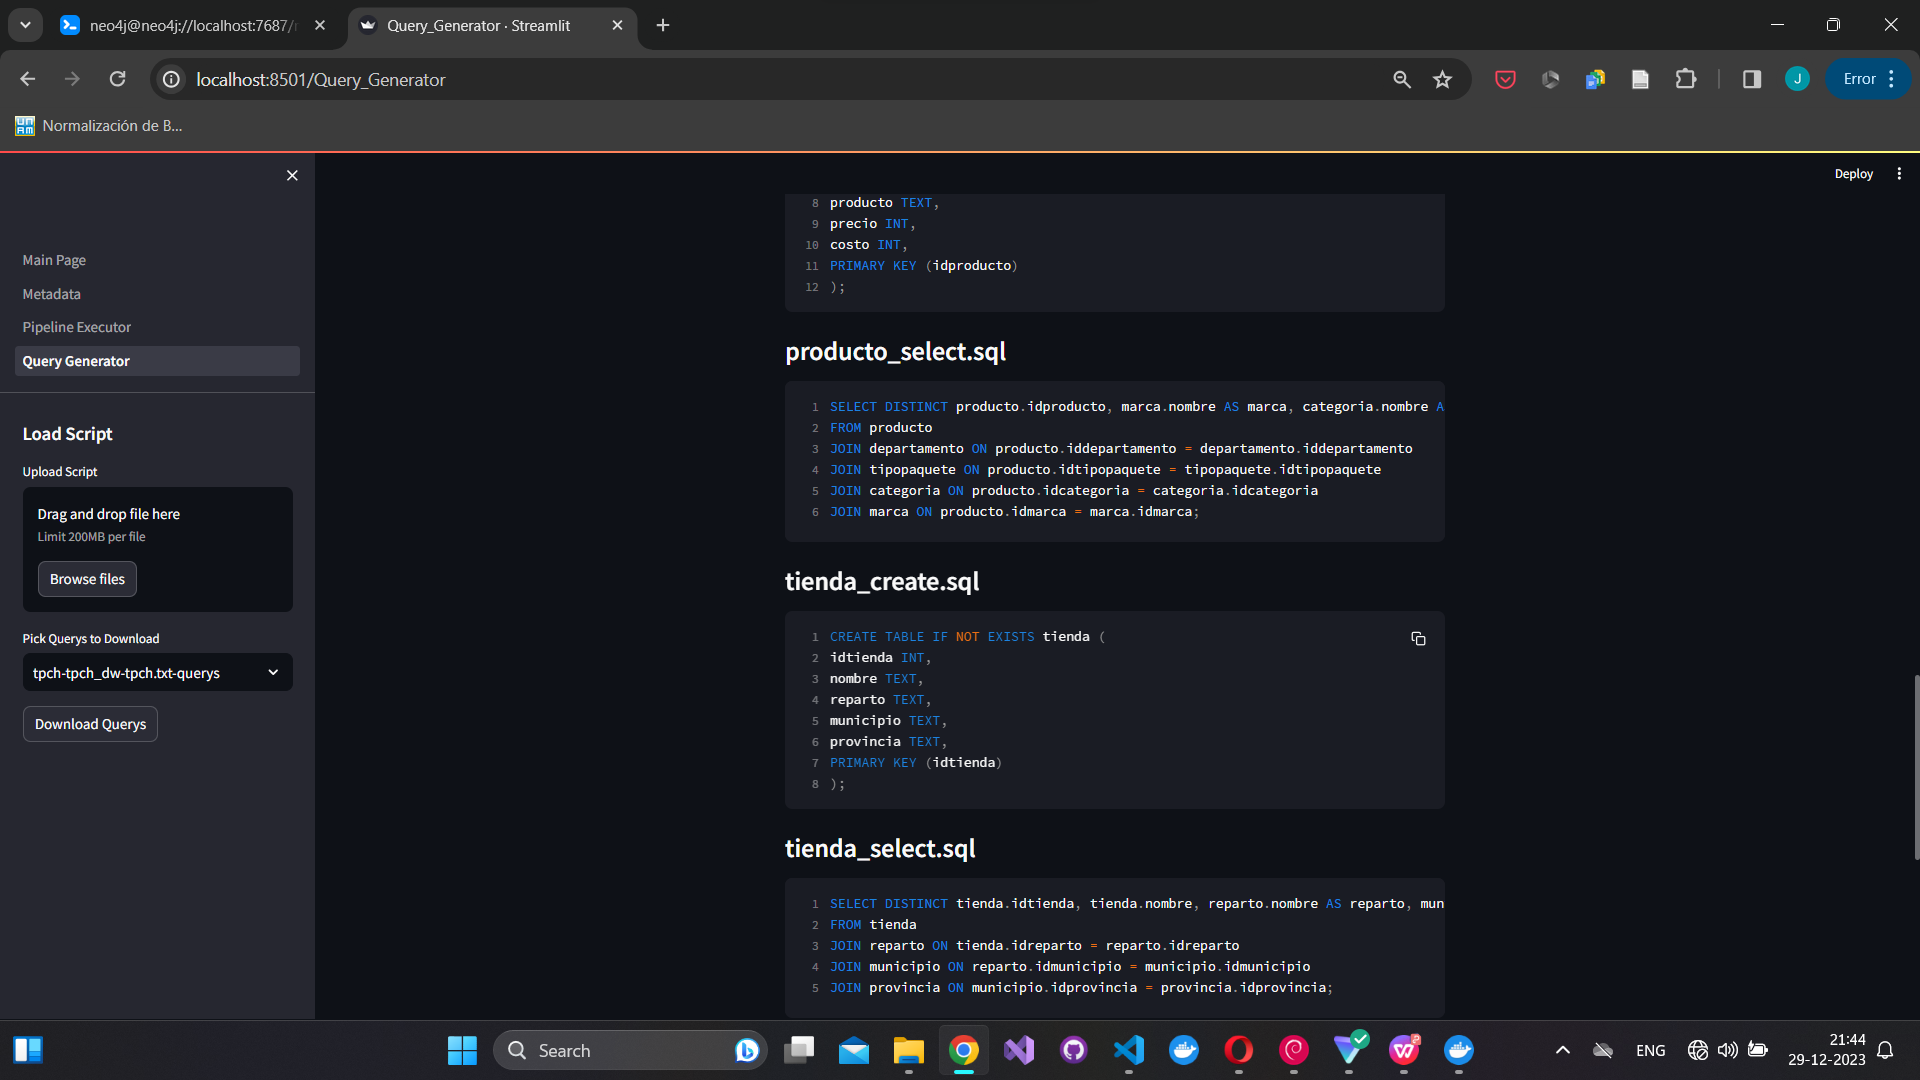
\includegraphics[scale=0.4]{Graphics/generatedquerys1.png}
        \caption{Fragmentos de consultas generadas.}
        \label{fig:qfragment}
    \end{figure}

    \begin{figure}
        \centering
        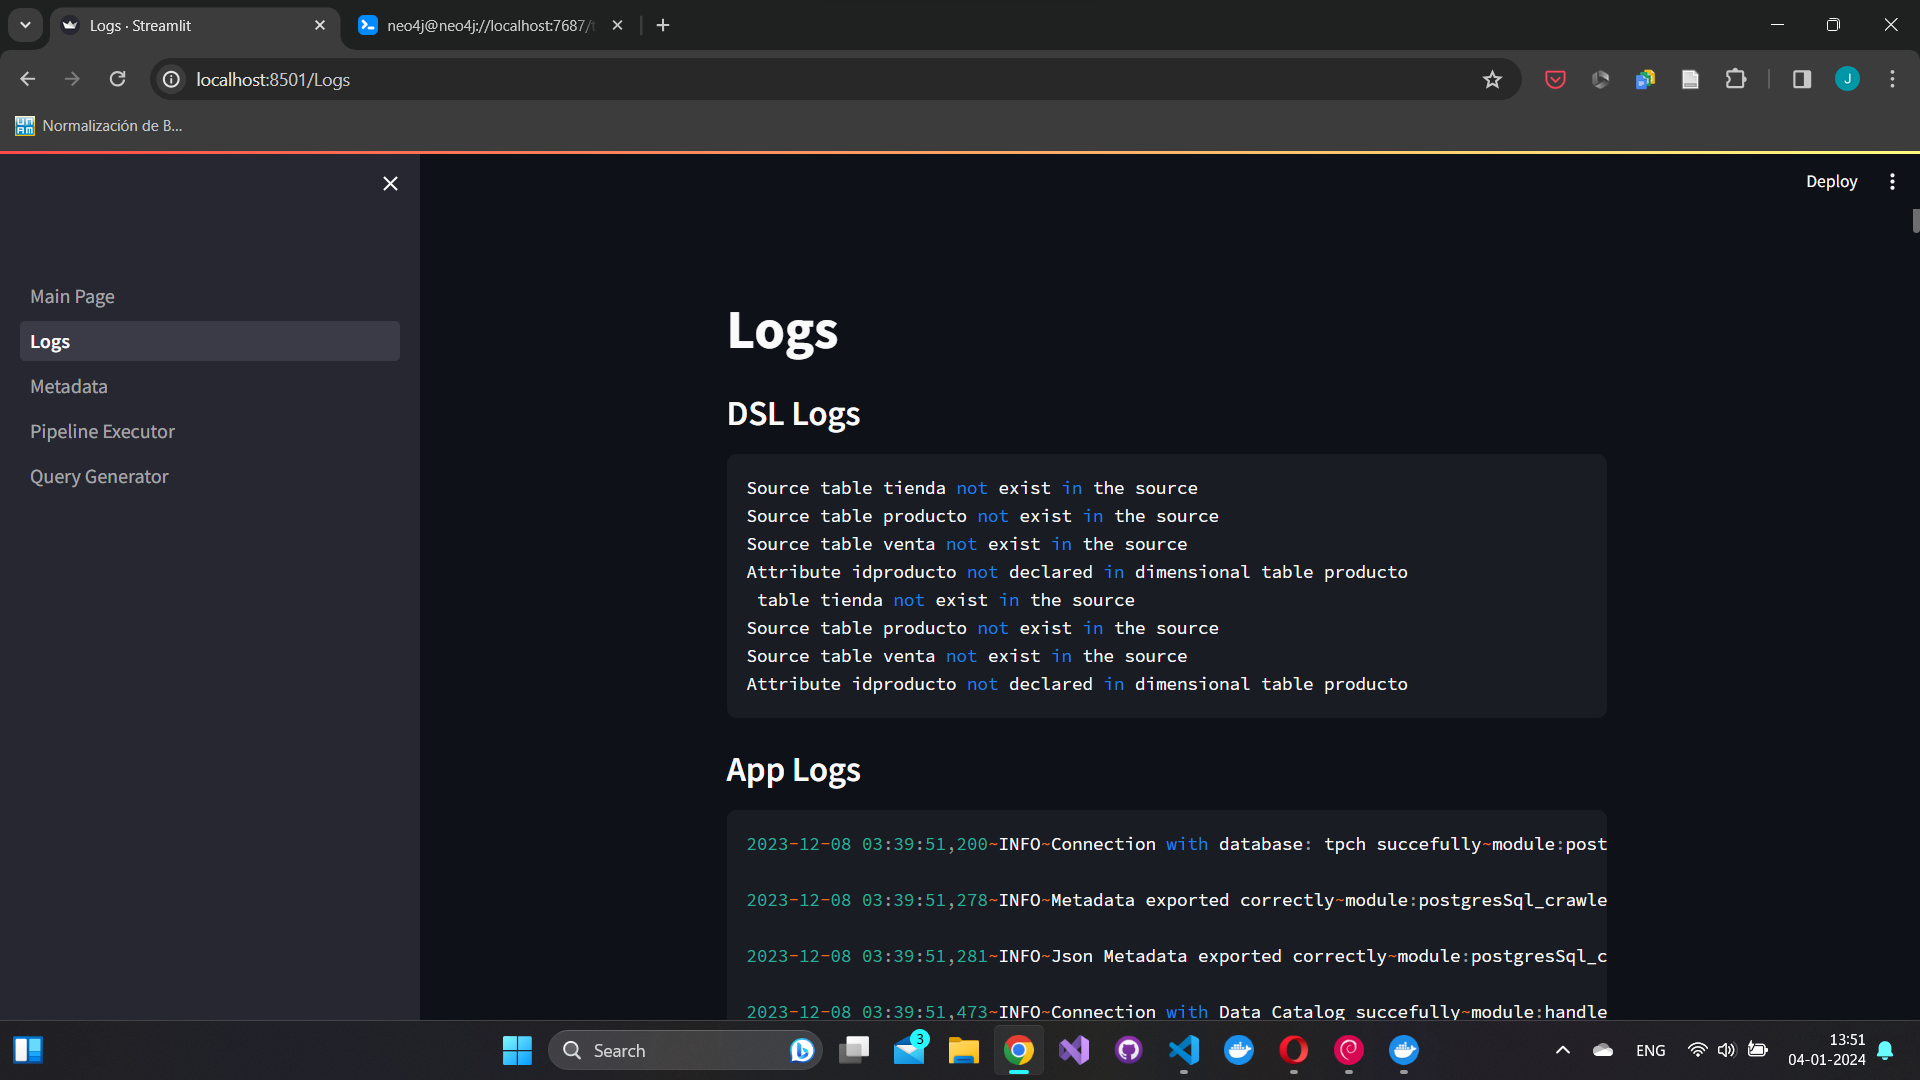
\includegraphics[scale=0.4]{Graphics/logs.png}
        \caption{Im\'agen de la p\'agina Logs.}
        \label{fig:logs}
    \end{figure}
\end{annexes}
%\printbibliography[heading=bibintoc]


\end{document}